\chapter{Rigid fluid coupling}
\label{chap:rfc}

\section{Introduction}
\label{sec:intro}
In the current chapter, we model the dynamics of rigid bodies in fluid flow and
the coupled behavior of fluid and rigid bodies. As part of AWJM, the behavior of
the abrasive particles in the fluid jet can be modeled by studying the
rigid-fluid coupling phenomenon.

Transport of arbitrarily shaped rigid bodies in fluid flows is a common
phenomenon that occurs widely in nature. Bodies transport in internal systems
\citep{Dai2021}, debris flow \citep{Qingyun2022}, the food processing industry
\citep{Karunasena2014}, and ice-sea modeling \citep{Mintu2018} are a few areas to
mention. The two-way coupling between the rigid and the fluid flow is nonlinear,
and a numerical study is chosen due to its flexibility in modeling the physics
accurately. Numerically rigid fluid coupling (RFC) can be studied with
mesh-based, or meshless techniques can be utilized.


In the current chapter, we couple CTVF with MDEM to handle the rigid fluid
coupling problems. The fluid phase is modeled using a corrected transport
velocity formulation developed by \citep{adepu2021corrected}. CTVF provides
smooth pressure distribution with EDAC formulation and homogeneous particle
distribution, resulting in accurate fluid modeling. Rigid-rigid interactions are
modeled with MDEM and is applied to 3D problems. A damping term is introduced
into the contact force model to account for the energy loss during the
collision. The interaction between the fluid phase and rigid bodies is handled
using the dummy particle approach \citep{Adami2012}.
% We explore different rigid fluid coupling strategies by simulating high
% density ratio simulations.
Numerical examples were simulated to validate the resulting RFC model, including
the water entry of a cube, a circular body, and two circular bodies in series in
a hydrostatic tank. Rigid-rigid interaction solver is validated using 2D and 3D
reference test cases with analytical and experimental solutions available. A
freely and controlled sliding body, a rolling cylinder, and the collapse of a
stack of cylinders under gravity are simulated.
% 3D body transport under a dam break event is studied as the main test  case.
The proposed MDEM-CTVF model has been found satisfactory in modeling
rigid-fluid coupling simulations with acceptable accuracy and performance. All
the results are fully automated with the automan package \citep{automan2018} and
made hundred percent reproducible. The source code for all the problems
demonstrated in this manuscript is made available at
\url{https://github.com/dineshadepu/rfc}.


\FloatBarrier%
\section{Rigid body dynamics}
\label{sec:rbd}
% The rigid body is discretized into particles with equal spacing each particle
% with mass $m_i$ and density $\rho_i$. Rigid body has a total 6 degrees of
% freedom (DOF), divided into $3$ translational and $3$ rotational.
The equations governing the dynamics of a rigid body are, balance of linear and
angular momentum given by,
\begin{equation}
  \label{eq:balance_linear_mom}
  \frac{d \; (M \ten{v}_{cm})}{d t} = \sum_i \ten{F}_i,
\end{equation}
\begin{equation}
  \label{eq:balance_angular_mom}
  \frac{d \ten{L}}{d t} = \teng{\tau}_{cm},
\end{equation}
where $M$, $\ten{v}_{cm}$ are the mass and velocity of the rigid body.
$\ten{F}_i, \teng{\tau}_{cm}, \ten{L} $ are force acting at point $i$, torque and
angular momentum about the center of mass of the rigid body. In the current
case, force acting on the particle $i$ ($\ten{F}_i$) is due to the interaction
with the other bodies and with the fluid particles, and any other body forces.
The torque ($\teng{\tau}_{cm}$) and angular momentum ($\ten{L}$) are computed as,
\begin{equation}
  \label{eq:torque}
 \teng{\tau}_{cm} = \sum_i \ten{F}_i \times (\ten{x}_{cm} - \ten{x}_{i}),
\end{equation}
\begin{equation}
  \label{eq:moi}
  \teng{L} =
  \sum_i \; \ten{r}_i \times \; (\teng{\omega} \times \ten{r}_i)
  = \sum_i \; m_i \; [(\ten{r}_i \cdot \ten{r}_i) \ten{I} - \ten{r}_i \otimes \ten{r}_i].
\end{equation}
Here $\ten{x}_{cm}$ and $\omega$ are the position of the center of mass and
angular velocity of the rigid body. $m_i$, $\ten{x}_{i}$, $\ten{r}_i$ are the
mass, position of particle, and vector from center of mass to the particle i.

\begin{figure}[!htpb]
  \centering
  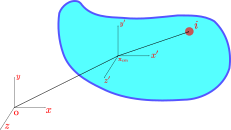
\includegraphics[width=0.7\textwidth]{images/rfc/images/rigid_body/rigid_body}
  \caption{Body frame and local frame description of rigid body}
  \label{fig:gloabl_body_frame_rb}
\end{figure}
We use two coordinate frames to capture the dynamics of the rigid body, a
global frame and a body frame as shown in
\cref{fig:gloabl_body_frame_rb}. The body fixed frame, which moves with
rigid body is located always at the center of mass ($\ten{x}_{cm}$). The
state of the rigid body at a given time ($t$) can be described using position
($\ten{x}_{cm}$) and velocity ($\ten{v}_{cm}$) of the center of mass, a
rotation matrix($\ten{R}$) to represent the orientation of the rigid body with
respect to the global frame, and angular velocity($\teng{\omega}$). The center
of mass is computed with
\begin{equation}
  \label{eq:center_of_mass}
  \ten{x}_{cm} = \frac{\sum_i m_i \; \ten{x}_{i} }{\sum_i m_i }
\end{equation}
The position of the discretized particle ($i$) in
\cref{fig:gloabl_body_frame_rb} belonging to the rigid body at time $t$ can be
computed ,
\begin{equation}
  \label{eq:rb_particle_pos_update}
  \ten{x}_i = \ten{x}_{cm} + \ten{r}_{i},
\end{equation}
with
\begin{equation}
  \label{eq:rb_particle_pos_update}
  \ten{r}_i = \ten{R} \cdot \overline{\ten{r}}_{i}.
\end{equation}
Here $\overline{\ten{r}}_{i}$ is the position of the particle $i$ about the body
frame axis and remains constant through out the simulation. The rotation matrix
$\ten{R}$ is used to bring the body frame position vector to the global frame
$\ten{O}$. Similarly the velocity vector is computed as,
\begin{equation}
  \label{eq:rb_particle_vel_update}
  \ten{v}_i = \ten{v}_{cm} + \teng{\omega} \times \ten{r}_{i}.
\end{equation}

We evolve the state of the rigid body through the integration of the
\cref{eq:balance_linear_mom,eq:balance_angular_mom}. The linear velocity of the
center of mass ($\ten{v}_{cm}$) and angular momentum ($\ten{L}$) at the next
timestep are computed as,
\begin{equation}
  \label{eq:lin_vel_cm_update}
  \ten{v}_{cm}^{n+1} = \ten{v}_{cm}^{n} + \frac{\ten{F}_{cm}}{M} \; \Delta t,
\end{equation}
\begin{equation}
  \label{eq:ang_mom_update}
  \ten{L}^{n+1} = \ten{L}^{n} + \teng{\tau}_{cm} \; \Delta t.
\end{equation}

The position of the center of mass and orientation ($\ten{R}$) are updated
by,
\begin{equation}
  \label{eq:lin_pos_cm_update}
  \ten{x}_{cm}^{n+1} = \ten{x}_{cm}^{n} + \ten{v}_{cm}^{n} \; \Delta t,\\
  \ten{R}^{n+1} = \ten{R}^{n} + \tilde{\teng{\omega}}^{n} \, \ten{R}^{n} \; \Delta t,
\end{equation}
where $\tilde{\teng{\omega}}^{n}$ is matrix formulation of angular velocity
$\omega$. The angular velocity at the new time step is computed with
\begin{equation}
  \label{eq:ang_velocity_update}
  \teng{\omega}^{n+1} = (\textit{\teng{I}}^{-1})^{n+1} \; \ten{L}^{n+1}.
\end{equation}
Here, moment of inertia at the new time step is computed as,
\begin{equation}
  \label{eq:moi_update}
  (\textit{\teng{I}}^{-1})^{n+1} = \ten{R}^{n+1} \textit{\teng{\overline{I}}}^{-1} (\ten{R}^{n+1})^T.
\end{equation}
where moment of inertia ($\textit{\teng{\overline{I}}}^{-1}$) in body frame is
used to compute in global frame at every time instant for faster computations.
The position and velocity of the particles of the rigid body are updated by
\begin{eqnarray}
  \label{eq:rb_particle_pos_update}
  \ten{r}_i = \ten{R} \cdot \overline{\ten{r}}_{i},\\
  \ten{x}_i = \ten{x}_{cm} + \ten{r}_{i},\\
  \ten{v}_i = \ten{v}_{cm} + \teng{\omega} \times \ten{r}_{i}.
\end{eqnarray}


\FloatBarrier%
\subsection{Contact algorithm}
\label{rfc:sec:contact-algorithm}
% \todoin{\cite{chen2019coupled} has damping model. Also he mentioned the parameters
% required in stack of cylinders example.}

\begin{figure}[!htpb]
  \centering
  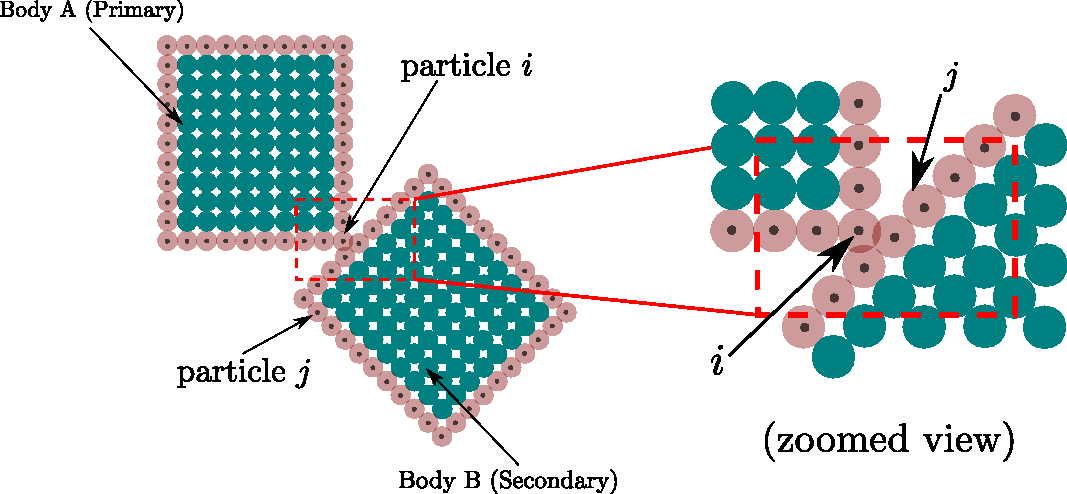
\includegraphics[width=1.0\textwidth]{images/rfc/images/contact_force/contact_force_description}
  \caption{Contact force description}
\label{fig:contact_foce_description}
\end{figure}
To handle the contact we mark the bodies under contact as primary and secondary.
Each body is discretized into equispaced points, each having mass equivalent to
their density times the volume spanned by the spacing. The force on each
particle is computed due to the interaction with the other body. The force is
computed on the primary body particles due to the interaction with the secondary
body and an equal and opposite force is transferred to the closest particle on
the secondary body. The force acting on particle $i$ due to the interaction with
body $B$, can be resolved into a normal and tangential part. Here, we utilize
\cite{mohseni2021particle} to compute these forces. Rather than computing the
force on particle $i$ due to each individual particle $j$, we consider the force
due to the full body $B$, with which we are able to consider the shape of the
body, and not computing the force by assuming the body's shape at the
interaction as being spherical. In traditional DEM, to compute the force on
particle $i$, we compute the overlap of particle $i$ with each and every
particle $j$ of body $B$, where both particle $i$ and $j$ are assumed to be
spherical in shape. This leads to inaccurate modeling of contact when the bodies
in interaction are not spherical in shape. We request the reader to see
\cite{mohseni2021particle}, and \citep{adepu_improved_2022} for clear
description.

The contact force is resolved into a normal and tagential part. The normal force
is used to eliminate the two bodies to penetrate, while the tangential part for
friction modeling. The normal force $\ten{F}_i$ due to the interaction with body
$B$ is computed as,
\begin{equation}
  \label{eq:contact-algorithm-normal}
  \ten{F}_i = K_r \delta_{n}^{i} \ten{n}_i.
\end{equation}
Here, to compute the overlap $\delta_{n}^{i}$, the distance ($d_i$) of particle $i$
from the boundary particles $j$ of body $B$ is used,
\begin{equation}
  \label{eq:cf-distance-computation}
  d_i = \frac{
    \displaystyle\sum\limits_{j = 1}^{\text{NP}^{b}} \;
    \big( \ten{n}_i \cdot \ten{x}_{ij} \big)  \frac{m_j}{\rho_j} W_{ij}}
  {
    \displaystyle\sum\limits_{j = 1}^{\text{NP}^{b}} \;
    \frac{m_j}{\rho_j} W_{ij}}.
\end{equation}
Here, the normal contact vector $\ten{n}_i$ is computed using
\begin{equation}
  \label{eq:cf-normal-vector}
  \ten{\hat{n}}_i = \frac{
    \displaystyle\sum\limits_{j = 1}^{\text{NP}^{j}} \;
    \frac{\ten{r}_{ij}}{r_{ij}}  \frac{m_j}{\rho_j} W_{ij}}
  {
    \displaystyle\sum\limits_{j = 1}^{\text{NP}^{j}} \;
    \frac{m_j}{\rho_j} W_{ij}},
\end{equation}
\begin{equation}
  \label{eq:cf-normal-vector}
  \ten{n}_i = \frac{\teng{\hat{n}}_i}{||\teng{\hat{n}}_i||}.
\end{equation}

Utilizing $d_i$, the overlap $\delta_{n}^{i}$ is computed by
\begin{equation}
  \label{eq:cf-overlap}
  \delta_{n}^{i} = \Delta x - d_i,
\end{equation}
where $\Delta x$ is the initial spacing between the particles. Note that while
computing the overlap of particle $i$ with the body $B$, we have computed an
effective overlap, rather than per particle interaction. This effectively is
able to model the interaction between non smooth surfaces, contrast from
particle particle force computation.

% \todoin{Write about damping}

To compute the tangential force, we associate a tangential spring attached to
particle $i$ and the interacting body $B$. The tangential spring is activated
when the particle comes into contact with body $B$, which is conformed by
\cref{eq:cf-overlap}. The magnitude of the tangential spring is initiated to
zero ($|\Delta \textit{\textbf{l}}_i|=0$) at the beginning of the contact. The
tangential force is history-dependent. The contact friction force is
proportional to the tangential spring displacement, which is integrated over
the contact time as
\begin{equation}
  \label{eq:tangential-force}
  \ten{F}_{i}^{t^{n+1}} =
  -k_f \Delta \textit{\textbf{l}}_i^{\,n + 1} =
  -k_f \big[\big(\Delta {\textit{\textbf{l}}}_i^{\,n} \
  + \ten{v}_{ij}^{n + 1} \Delta t\big) \cdot \ten{t}_i^{n + 1} \big] \
  \ten{t}_i^{n + 1},
\end{equation}
where $\Delta t$ is the time step, $\ten{v}_{ij} = \ten{v}_{i} - \ten{v}_j$ is
the relative velocity of the primary particle $i$ with respect to the
secondary particle $j$. The tangential unit vector is computed by,
\begin{equation}
  \label{eq:tangential-vect}
  \ten{t}_i = \frac{\ten{v}_{ij} - (\ten{v}_{ij} \cdot \ten{n}_i) \ten{n}_i}{|\ten{v}_{ij} - (\ten{v}_{ij} \cdot \ten{n}_i) \ten{n}_i|}.
\end{equation}

Sliding friction condition between the interacting solids is imposed through
the Coulomb's law, this is done by coupling the tangential force with the
normal force as,
\begin{equation}
  \label{eq:Coulomb-law}
  \ten{F}_{i}^{t} = \min(\mu |\ten{F}_{i}^{n}|, |\ten{F}_{i}^{t}|) \
  \frac{\ten{F}_{i}^{t}}{|\ten{F}_{i}^{t}|}.
\end{equation}
The total force acting on the particle $i$ due to the
interaction with body $B$ is:
\begin{equation}
  \label{eq:contact-force}
  \ten{F}_{i}^{cont} = \ten{F}_{i}^{n} + \ten{F}_{i}^{t}
\end{equation}

\begin{figure}[!htpb]
  \centering
  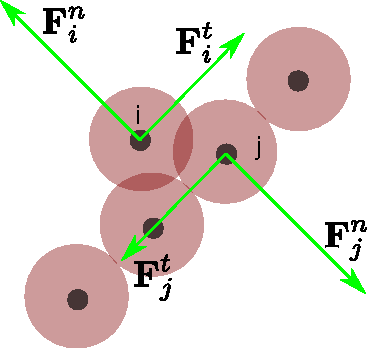
\includegraphics[width=0.3\textwidth]{images/rfc/images/contact_force/contact_force_description_3}
  \caption{Force transfer to the secondary particles $j$ from the primary body particle $i$}
\label{fig:rfc:secondary_particle_contact_foce_transfer}
\end{figure}
An equal and opposite force of the same magnitude is applied to the closest
secondary particle $j$ of $i$ (\cref{fig:rfc:secondary_particle_contact_foce_transfer}),
\begin{equation}
  \label{eq:contact-force}
  \ten{F}_{j}^{cont} = - \ten{F}_{i}^{cont}
\end{equation}

\FloatBarrier%
\section{Fluid phase modeling}
\label{sec:rfc:fluid-dynamics}
To model the fluid phase, we use CTVF \cite{adepu2021corrected} scheme. According
to CTVF, the discretized continuity and momentum equation are:
\begin{equation}
  \label{eq:sph-discretization-continuity}
  \frac{\tilde{d}\rho_a}{dt} = \sum_{b} \; \frac{m_b}{\rho_{b}} \; (
  \rho_{a} \; \tilde{\ten{u}}_{ab} \; + \;
  (\rho \; (\tilde{\ten{u}} \; - \;
  \ten{u}))_{ab}) \; \cdot \nabla_{a} W_{ab},
\end{equation}
\begin{multline}
  \label{eq:sph-momentum-fluid}
  \frac{\tilde{d}\ten{u}_{a}}{dt} = - \sum_{b} m_b \bigg[
  \bigg(\frac{p_a}{\rho_a^2} + \frac{p_b}{\rho_b^2}\bigg) \ten{I} -
  \bigg(\frac{\ten{A}_a}{\rho_a^2} + \frac{\ten{A}_b}{\rho_b^2}
  \bigg) \bigg]
  \cdot \nabla_{a} W_{ab} \\
  + \ten{u}_{a} \sum_{b} \frac{m_b}{\rho_{b}} \; \tilde{\ten{u}}_{ab} \cdot
  \nabla_{a} W_{ab} + \sum_{b} m_b \frac{4 \eta \nabla W_{ab}\cdot
    \ten{r}_{ab}}{(\rho_a + \rho_b) (r_{ab}^2 + 0.01 h_{ab}^2)} \ten{u}_{ab} +
  \ten{g}_{a},
\end{multline}
where $\rho$, $m$, $p$ refer to the is the density, mass, and the pressure
respectively. $\ten{g}$ represents the gravitational acceleration and $\eta$ is
the kinematic viscosity of the fluid.


where $\ten{A}_a = \rho_a \ten{u}_a \otimes (\ten{\tilde{u}}_a - \ten{u}_a)$,
$\ten{I}$ is the identity matrix, $\eta$ is the kinematic viscosity of the fluid
and \cite{morris1997modeling} formulation is used to discretize the viscosity
term. We add to the momentum equation an additional artificial viscosity term
$\Pi_{ab}$~\citep{monaghan-review:2005} to maintain the stability of the
numerical scheme, given as,
\begin{align}
  \label{eq:mom-av}
  \Pi_{ab} =
  \begin{cases}
\frac{-\alpha h_{ab} \bar{c}_{ab} \phi_{ab}}{\bar{\rho}_{ab}}
  & \ten{u}_{ab}\cdot \ten{r}_{ab} < 0, \\
  0 & \ten{u}_{ab}\cdot \ten{r}_{ab} \ge 0,
\end{cases}
\end{align}
where,
%
\begin{equation}
  \label{eq:av-phiij}
  \phi_{ab} = \frac{\ten{u}_{ab} \cdot \ten{r}_{ab}}{r^2_{ab} + 0.01 h^2_{ab}},
\end{equation}
%
where $\ten{r}_{ab} = \ten{r}_a - \ten{r}_b$, $\ten{u}_{ab} = \ten{u}_a -
\ten{u}_b$, $h_{ab} = (h_a + h_b)/2$, $\bar{\rho}_{ab} = (\rho_a + \rho_b)/2$,
$\bar{c}_{ab} = (c_a + c_b) / 2$, and $\alpha$ is the artificial
viscosity parameter.

For a smoother pressure distribution we use EDAC equation,
\begin{multline}
  \label{eq:sph-discretization-edac}
  \frac{\tilde{d}p_a}{dt} = \sum_{b} \; \frac{m_b}{\rho_{b}} \; \bigg(
  (p_{a} - \rho_{a} c_{s}^2) \; \ten{u}_{ab} \; + \;
  p_{a} \; \tilde{\ten{u}}_{ab} \; - \;
  (p \; (\tilde{\ten{u}} - \ten{u}))_{ab} \; + \; \\
  4 \; \nu_{edac}
  \frac{p_a - p_b}{(\rho_a + \rho_b) (r^2_{ab} + 0.01 h_{ab}^{2})} \ten{r}_{ab}
  \bigg) \; \cdot \nabla_{a} W_{ab}.
\end{multline}

The particles are moved with a transport velocity for a homogenized particle
distribution, where the transport velocity is computed as,
\begin{equation}
  \label{eq:transport_velocity_position_derivative}
  \frac{d\ten{r}_a}{dt} = \ten{\tilde{u}}_a.
\end{equation}
%
The transport velocity is updated using,
\begin{equation}
  \label{eq:transport_velocity}
  \ten{\tilde{u}}_a(t + \Delta t) =\ten{u}_a(t) + \Delta t \; \frac{\tilde{d} \ten{u}_a}{dt} +
  \bigg(\frac{d \ten{u}_{a}}{dt}\bigg)_{\text{c}} \Delta t,
\end{equation}
%
where $\big(\frac{d \ten{u}_a}{dt}\big)_{\text{c}}$ is the homogenization
acceleration which ensures that the particle positions are homogeneous.
is a displacement based technique due to \cite{sun2017deltaplus},
\begin{equation}
  \label{eq:sun2019_pst}
  \bigg(\frac{d \ten{u}_a}{dt}\bigg)_{\text{c}} = - \frac{\text{Ma} \;
    (2h) c_0}{\Delta t} \sum_b \bigg[1 + R \bigg( \frac{W_{ab}}{W(\Delta x)} \bigg)^n
  \bigg] \nabla_a W_{ab} V_b,
\end{equation}
where $R$ is an adjustment factor to handle the tensile instability, and
$\text{Ma}$ is the mach number of the flow. $V_b$ is the volume of the
$b$\textsuperscript{th} particle. The acceleration is changed to account for
particles that are on the free surface. We use $R = 0.2$ and $n = 4$ as
suggested by \cite{sun_consistent_2019}. Further, the homogenization force
has to be adjusted at the free surface,
\begin{equation}
 \label{eq:shifting_force_free_surface_adjust_sun2019}
 \bigg(\frac{d \ten{u}_a}{dt}\bigg)_{\text{c}} =\begin{cases}
   0& \text{if boundary},\\
   \big(\frac{d \ten{u}_a}{dt}\big)_{\text{c}}  - (\big(\frac{d \ten{u}_a}{dt}\big)_{\text{c}} \cdot \ten{n}_a) \ten{n}_a& \text{if $h_b < h$},\\
   \big(\frac{d \ten{u}_a}{dt}\big)_{\text{c}}& \text{if $h_b = h$}.
 \end{cases}
\end{equation}
Where we have utilized the free surface identification scheme provided by \citep{adepu2021corrected}.

% \newpage
% ~\newpage
% ~\newpage

\subsection{Boundary conditions}
The dummy particle approach of \cite{Adami2012} is used to model the
boundaries. We use three layers of dummy particles to model the solid wall.
The properties of the solid wall are interpolated from the fluid particles.

When computing the divergence of the velocity field on fluid particles, we
enforce a no-penetration boundary condition and not a no-slip boundary
condition. The velocity of the fluid is projected onto the ghost particles
using,
\begin{equation}
  \label{eq:v-ghost}
  \ten{\hat{u}}_a = \frac{\sum_b\ten{u}_b W_{ab}}{\sum_b W_{ab}},
\end{equation}
\begin{equation}
  \label{eq:v-hat-ghost}
  \ten{\check{u}}_a = \frac{\sum_b\tilde{\ten{u}}_b W_{ab}}{\sum_b W_{ab}},
\end{equation}
where $\ten{u}_b$, $\ten{\tilde{u}}_b$ are the momentum and transport velocity
of the fluid respectively and $W_{ab}$ is the kernel value between the fluid
particle and the ghost particle.

The normal component of this projected velocity is then reflected and set as
the ghost particle velocity,
\begin{equation}
  \label{eq:free-slip-bc-u}
  \ten{u}_{\text{Ga}} = 2 \ten{\hat{n}}((\ten{u}_{\text{p}} - \ten{\hat{u}}_{\text{a}})\cdot \ten{\hat{n}}) + \ten{\hat{u}}_{\text{a}},
\end{equation}
where $\ten{u}_{\text{p}}$ is the local velocity of the boundary and
$\ten{\hat{n}}$ is the unit normal to the boundary particle $a$. Similarly the
transport velocity of the ghost particle is set as,
\begin{equation}
  \label{eq:free-slip-bc-u}
  \tilde{\ten{u}}_{\text{Gi}} = 2 \ten{\hat{n}}((\ten{u}_{\text{p}} - \ten{\check{u}}_{\text{i}})\cdot \ten{\hat{n}}) + \ten{\check{u}}_{\text{i}},
\end{equation}

When the viscous force is computed, the no slip boundary condition is used,
where the velocity on the boundary set as,
\begin{equation}
  \label{eq:no-slip-bc-u}
  \ten{u}_{\text{Ga}} = 2 \ten{u}_{\text{p}} - \ten{\hat{u}}_{\text{a}},
\end{equation}
a similar form is used for the transport velocity here too,
\begin{equation}
  \label{eq:no-slip-bc-uhat}
  \tilde{\ten{u}}_{\text{Ga}} = 2 \ten{u}_{\text{p}} - \ten{\check{u}}_{\text{a}}.
\end{equation}

The pressure of the boundary particle is extrapolated from its surrounding
fluid particles by the following equation,
\begin{equation}
  \label{eq:pressure-bc}
  p_w = \frac{\Sigma_f p_f W_{wf} + (\ten{g} - \ten{a}_{\ten{w}}) \cdot \Sigma_f
    \rho_f \ten{r}_{wf} W_{wf}}{\Sigma_f W_{wf}},
\end{equation}
where $\ten{a}_w$ is the acceleration of the wall. The subscript $f$ denotes
the fluid particles and $w$ denotes the wall particles.

\FloatBarrier%
\subsection{Rigid fluid coupling}\label{subsec:rfc}
The interaction between the fluid and the rigid body are handled using the dummy
particle approach of \citep{Adami2012}. The particles of the rigid body are
assumed as dummy particles with hydrodynamics properties of mass and density
while interacting with the fluid particles. We set the pressure of the boundary
particles from the extrapolated equation \citep{Adami2012} as,
\begin{equation}
  \label{eq:pressure-bc}
  p_s = \frac{\Sigma_f p_f W_{sf} + (\ten{g} - \ten{a}_{\ten{s}}) \cdot \Sigma_f
    \rho_f \ten{r}_{sf} W_{sf}}{\Sigma_f W_{sf}}.
\end{equation}
Here, $\ten{a}_s$ is the acceleration of the rigid body particles. The
subscript $f$ denotes the fluid and $s$ the rigid body particles. Using the
extrapolated pressure, the hydrodynamic density and mass of rigid body
particle is set as,
\begin{equation}
  \label{eq:pressure-bc}
  \rho_{s0} = p_s / c_0^2 + \rho_0
\end{equation}
\begin{equation}
  \label{eq:pressure-bc}
  m_{s0} = \rho_{s0} V_{s}
\end{equation}
Here the volume of the particle remains same, and is set to $\text{dx}^2$ in two
dimensions and $\text{dx}^3$ in three dimensions.

By utilizing the previously set hydrodynamic properties on the rigid body, the
interaction force is computed using,
\begin{equation}
  \ten{F}_{\text{RFC}}^i = -m_i \sum_{s} m_s \left(\frac{p_i}{\rho_{i}^2} +
  \frac{p_s}{\rho_{s}^2} \right) \nabla_{i} W(x_{is})
\end{equation}
where $i$ is fluid particle, $s$ is particle of rigid body.


\subsection{Time integration}

We use the kick-drift-kick scheme for the time integration. We first move the
velocities of the particles to half time step,
\begin{equation}
  \label{eq:velocity-update-stage-1}
  \ten{u}_a^{n+\frac{1}{2}} = \ten{u}_a^{n} + \frac{\Delta t}{2} \bigg(\frac{\tilde{d}\ten{u}_{a}}{dt}\bigg)^n,
\end{equation}

\begin{equation}
  \label{eq:velocity-hat-update-stage-1}
  \ten{\tilde{u}}_a^{n+\frac{1}{2}} = \ten{u}_a^{n+\frac{1}{2}} + \frac{\Delta t}{2} \bigg(\frac{d\ten{u}_{a}}{dt}\bigg)^{n}_{c}.
\end{equation}
%
Then the time derivatives of density and pressure are calculated using the
\cref{eq:sph-discretization-continuity} and \cref{eq:sph-discretization-edac}.
The new time step density, pressure and particle position are updated by,
\begin{equation}
  \label{eq:density-update-stage-2}
  \rho_{a}^{n+1} = \rho_{a}^{n} + \Delta t \; \bigg(\frac{\tilde{d}\rho_{a}}{dt}\bigg)^{n+\frac{1}{2}},
\end{equation}

\begin{equation}
  \label{eq:pressure-update-stage-2}
  p_{a}^{n+1} = p_{a}^{n} + \Delta t \; \bigg(\frac{\tilde{d}p_{a}}{dt}\bigg)^{n+\frac{1}{2}},
\end{equation}

\begin{equation}
  \label{eq:position-update-stage-2}
  \ten{r}_{a}^{n+1} = \ten{r}_{a}^{n} + \Delta t \; \ten{\tilde{u}}_{a}^{n+1}.
\end{equation}
%
Finally, at new time-step particle position, the momentum velocity is updated
\begin{equation}
  \label{eq:velocity-update-stage-3}
  \ten{u}_a^{n+1} = \ten{u}_a^{n+\frac{1}{2}} + \frac{\Delta t}{2} \bigg(\frac{\tilde{d}\ten{u}_{a}}{dt}\bigg)^{n+1}.
\end{equation}


For the numerical stability of fluid phase, the time step depends on the CFL condition as,
\begin{equation}
  \label{eq:time-step-cfl}
  (\Delta t)_{\text{fluid}} = \mathrm{min} \bigg( 0.25 \; \frac{h}{c + |U|} ,  0.25 \; \frac{h^2}{\nu},  0.25 \; \frac{h^2}{g} \bigg),
\end{equation}
where $|U|$ is the maximum velocity magnitude, $c$ is the speed of sound
typically chosen as $10 |U|$ for fluids in this work. For rigid body, the time
step is constrained as,
\begin{equation}
  \label{eq:time-step-body-force}
  (\Delta t)_{\text{rb}} \leq \frac{\pi}{50} \sqrt{\frac{m}{K_r}}.
\end{equation}
We choose minimum of both the phases fields for a stable simulation as following,
\begin{equation}
  \label{eq:time-step-body-force}
  \Delta t = min((\Delta t)_{\text{fluid}}, (\Delta t)_{\text{rb}})
\end{equation}



% ==============================
% ==============================
% ==============================
% ==============================
% ==============================
% ==============================
% ==============================
% \FloatBarrier%
% \section{Final set of governing equations}
% \label{sec:final_discretized_equations}


% \begin{itemize}
% \item Write the time step factor.
% \item Write the rigid body equations with real forces.
% \item Write rigid body particle equations.
% \end{itemize}

% \begin{multline}
%   \label{eq:sph-momentum-fluid}
%   \frac{\tilde{d}\ten{u}_{a}}{dt} = - \sum_{b \in b_f} m_b \bigg[
%   \bigg(\frac{p_a}{\rho_a^2} + \frac{p_b}{\rho_b^2}\bigg) \ten{I} -
%   \bigg(\frac{\ten{A}_a}{\rho_a^2} + \frac{\ten{A}_b}{\rho_b^2}
%   \bigg) + \Pi_{ab} \bigg]
%   \cdot \nabla_{a} W_{ab} \\
%   + \ten{u}_{a} \sum_{b \in b_f} \frac{m_b}{\rho_{b}} \; \tilde{\ten{u}}_{ab} \cdot
%   \nabla_{a} W_{ab} + \sum_{b \in b_f} m_b \frac{4 \eta \nabla W_{ab}\cdot
%     \ten{r}_{ab}}{(\rho_a + \rho_b) (r_{ab}^2 + 0.01 h_{ab}^2)} \ten{u}_{ab} \\
%  - \sum_{b \in b_r} m_b \bigg[
%   \bigg(\frac{p_a}{\rho_a^2} + \frac{p_b}{\rho_b^2}\bigg) \ten{I} -
%   \bigg(\frac{\ten{A}_a}{\rho_a^2} + \frac{\ten{A}_b}{\rho_b^2}
%   \bigg) + \Pi_{ab} \bigg]
%   \cdot \nabla_{a} W_{ab} \\
%   + \ten{u}_{a} \sum_{b \in b_r} \frac{m_b}{\rho_{b}} \; \tilde{\ten{u}}_{ab} \cdot
%   \nabla_{a} W_{ab} + \sum_{b \in b_r} m_b \frac{4 \eta \nabla W_{ab}\cdot
%     \ten{r}_{ab}}{(\rho_a + \rho_b) (r_{ab}^2 + 0.01 h_{ab}^2)} \ten{u}_{ab}\\
%  - \sum_{b \in b_b} m_b \bigg[
%   \bigg(\frac{p_a}{\rho_a^2} + \frac{p_b}{\rho_b^2}\bigg) \ten{I} -
%   \bigg(\frac{\ten{A}_a}{\rho_a^2} + \frac{\ten{A}_b}{\rho_b^2}
%   \bigg) + \Pi_{ab} \bigg]
%   \cdot \nabla_{a} W_{ab} \\
%   + \ten{u}_{a} \sum_{b \in b_b} \frac{m_b}{\rho_{b}} \; \tilde{\ten{u}}_{ab} \cdot
%   \nabla_{a} W_{ab} + \sum_{b \in b_b} m_b \frac{4 \eta \nabla W_{ab}\cdot
%     \ten{r}_{ab}}{(\rho_a + \rho_b) (r_{ab}^2 + 0.01 h_{ab}^2)} \ten{u}_{ab}
%   + \ten{g}_{a}
% \end{multline}


% The particles in the current scheme are moved with the transport velocity,
% \begin{equation}
%   \label{eq:transport_velocity_position_derivative}
%   \frac{d\ten{r}_a}{dt} = \ten{\tilde{u}}_a.
% \end{equation}


% \todoin{Rigid body equations}
% \todoin{Expand on forces in detail}
% \begin{equation}
%   \label{eq:balance_linear_mom}
%   \frac{d \; (M \ten{v}_{cm})}{d t} = \sum_i \ten{F}_{due to fluid} \sum_i \ten{F}_{due to solids}
% \end{equation}

% \begin{equation}
%   \label{eq:balance_angular_mom}
%   \frac{d \ten{L}}{d t} = \sum_i \ten{F}_{due to fluid} \sum_i \ten{F}_{due to solids} \times (\ten{r}_{cm} - \ten{r}_{i})
% \end{equation}


% \begin{equation}
%   \label{eq:rb_particle_pos_update}
%   \ten{x}_i(t) = \ten{x}_{cm}(t) + \ten{R}(t) \; \hat{\ten{r}}_{i}(t)
% \end{equation}


% \begin{equation}
%   \label{eq:rb_particle_vel_update}
%   \ten{v}_i(t) = \ten{v}_{cm}(t) + \teng{\omega}(t) \; \ten{r}_{i}(t)
% \end{equation}

% ==============================
% ==============================
% ==============================
% ==============================
% ==============================
% ==============================
% ==============================


\FloatBarrier%
\section{Results and discussion}
\label{sec:results}

% \subsection{3D Bouncing cube on a wall under gravity}
% \label{sec:bouncing-cube}

\FloatBarrier%
\subsection{Cylinder rolling on an inclined plane}
\label{sec:cylinder-rolling-on-an-inclined-plane}
A cylinder of diameter $1.0$ m rolling on an inclined plane under gravity is
simulated in the current test case. The physical model is shown in
\cref{fig:circular-body:schematic-1}, while the computational model is in
\cref{fig:circular-body:schematic-2}. In the computational model the $x$-axis
points in the direction of the slope, where the gravity makes an angle $\theta$
with the vertical. The physical and the numerical parameters are given in
\cref{tab:circular-body-rolling-params}. A total of two friction coefficients
are simulated. Analytical expression of the variation of the center of mass of
the cylinder with time is,
\begin{align}
  \label{eq:analytical-x-cm-rolling-cylinder}
  x_{cm}(t) =
  \begin{cases}
  x_0 + \frac{1}{2} \, g \, t^2 \, (\sin(\theta) - \mu \cos(\theta)) & \tan{\theta} > 3.5\mu,\\
  x_0 + \frac{1}{3} \, g \, t^2 \, \sin(\theta) & \tan{\theta} \leq 3.5\mu.
\end{cases}
\end{align}
Here, $x_0$ is the initial position of the center of mass of the cylinder.
\begin{figure}[!htpb]
  \centering
  \begin{subfigure}{0.48\textwidth}
    \centering
    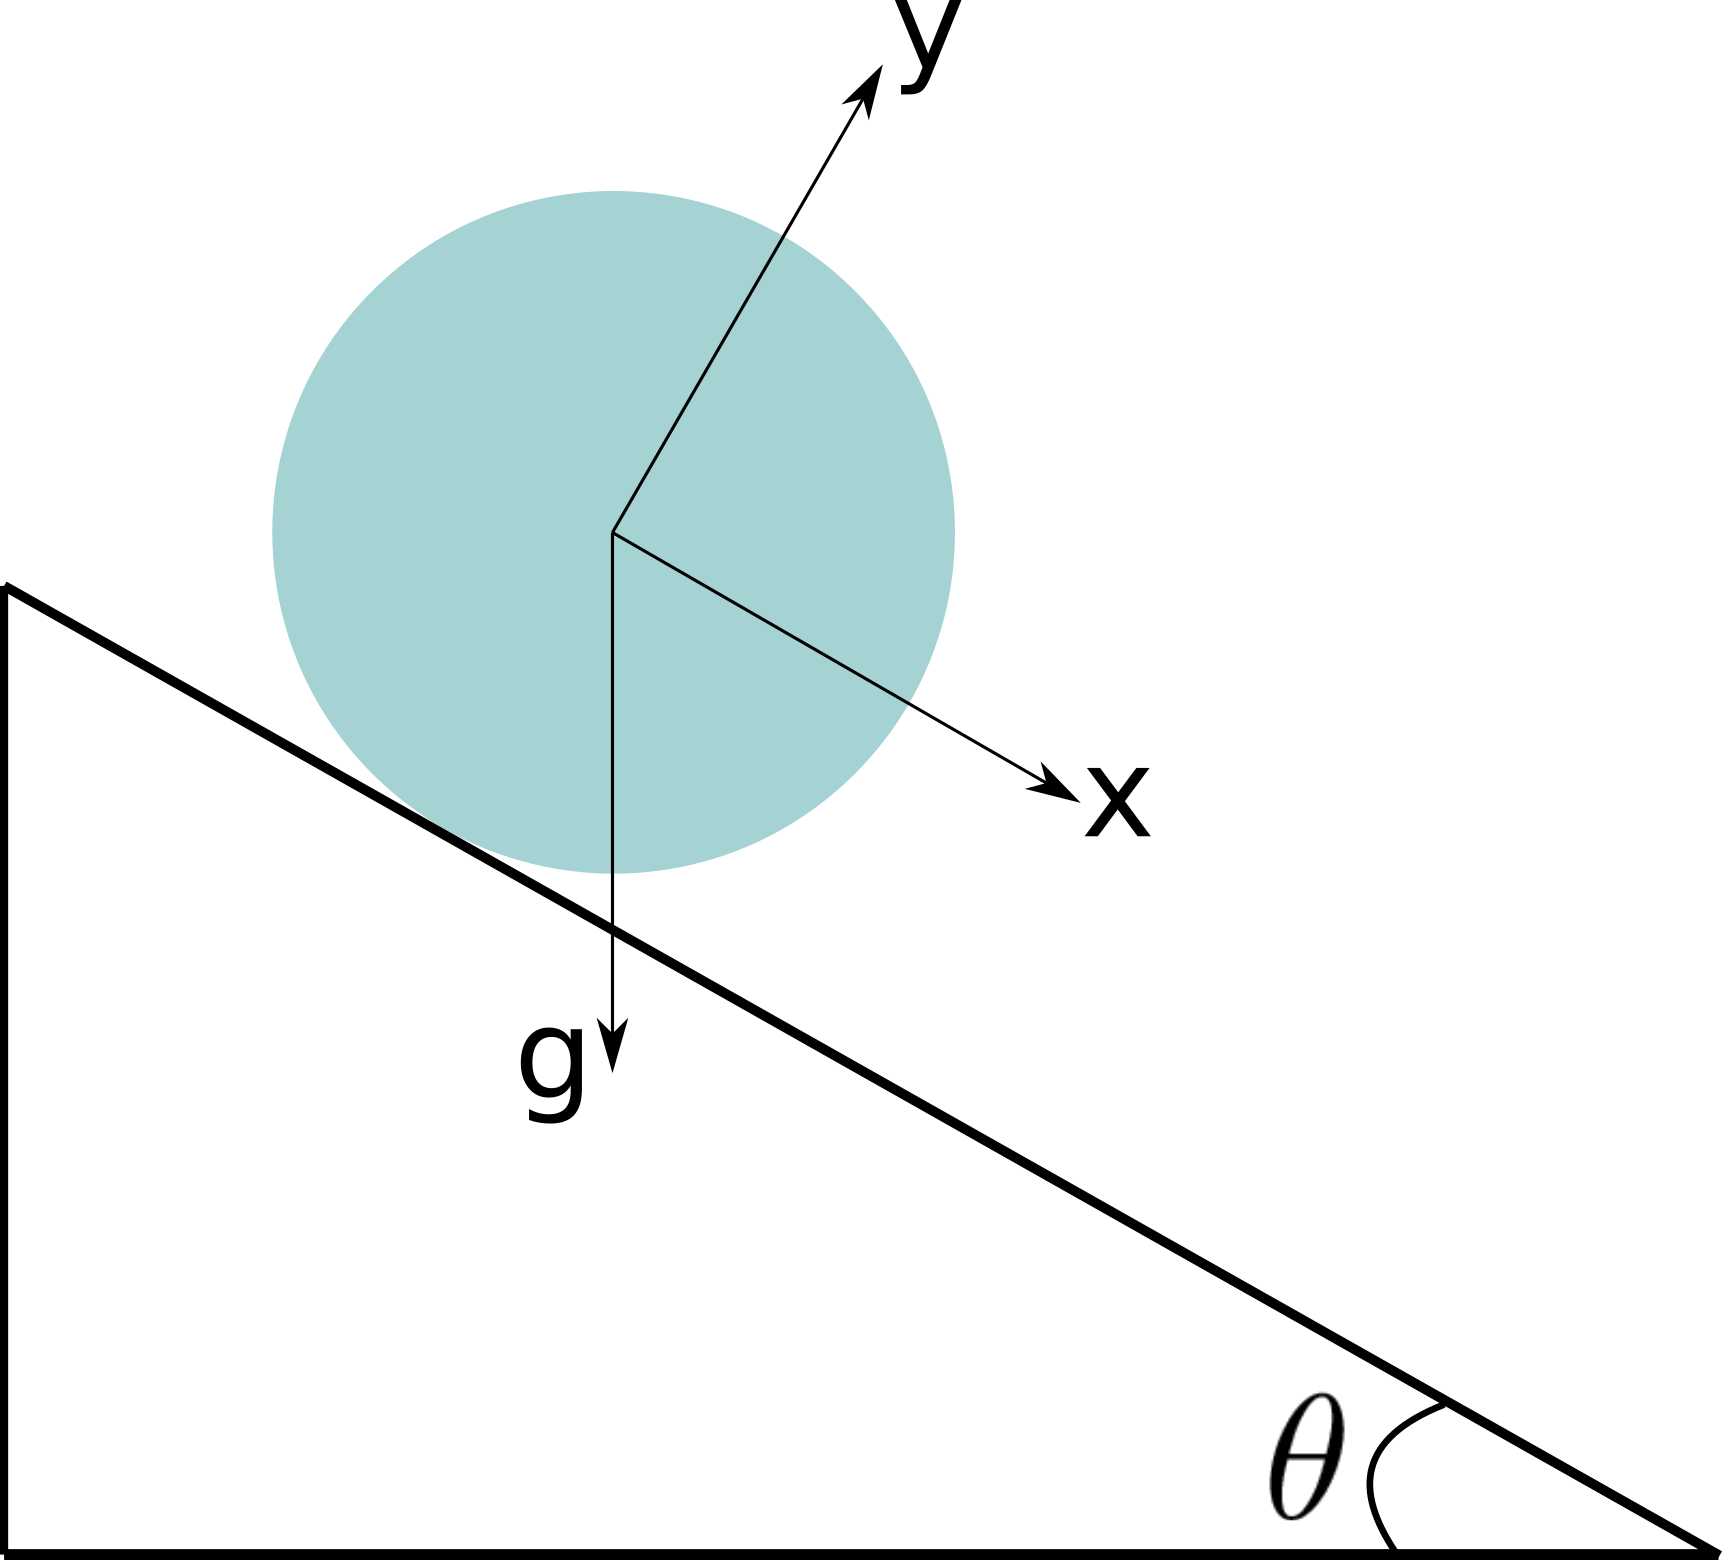
\includegraphics[width=1.0\textwidth]{images/rfc/images/de_2021_cylinder_rolling_on_an_inclined_plane/schematic_1}
    \subcaption{}\label{fig:circular-body:schematic-1}
  \end{subfigure}
  \begin{subfigure}{0.48\textwidth}
    \centering
    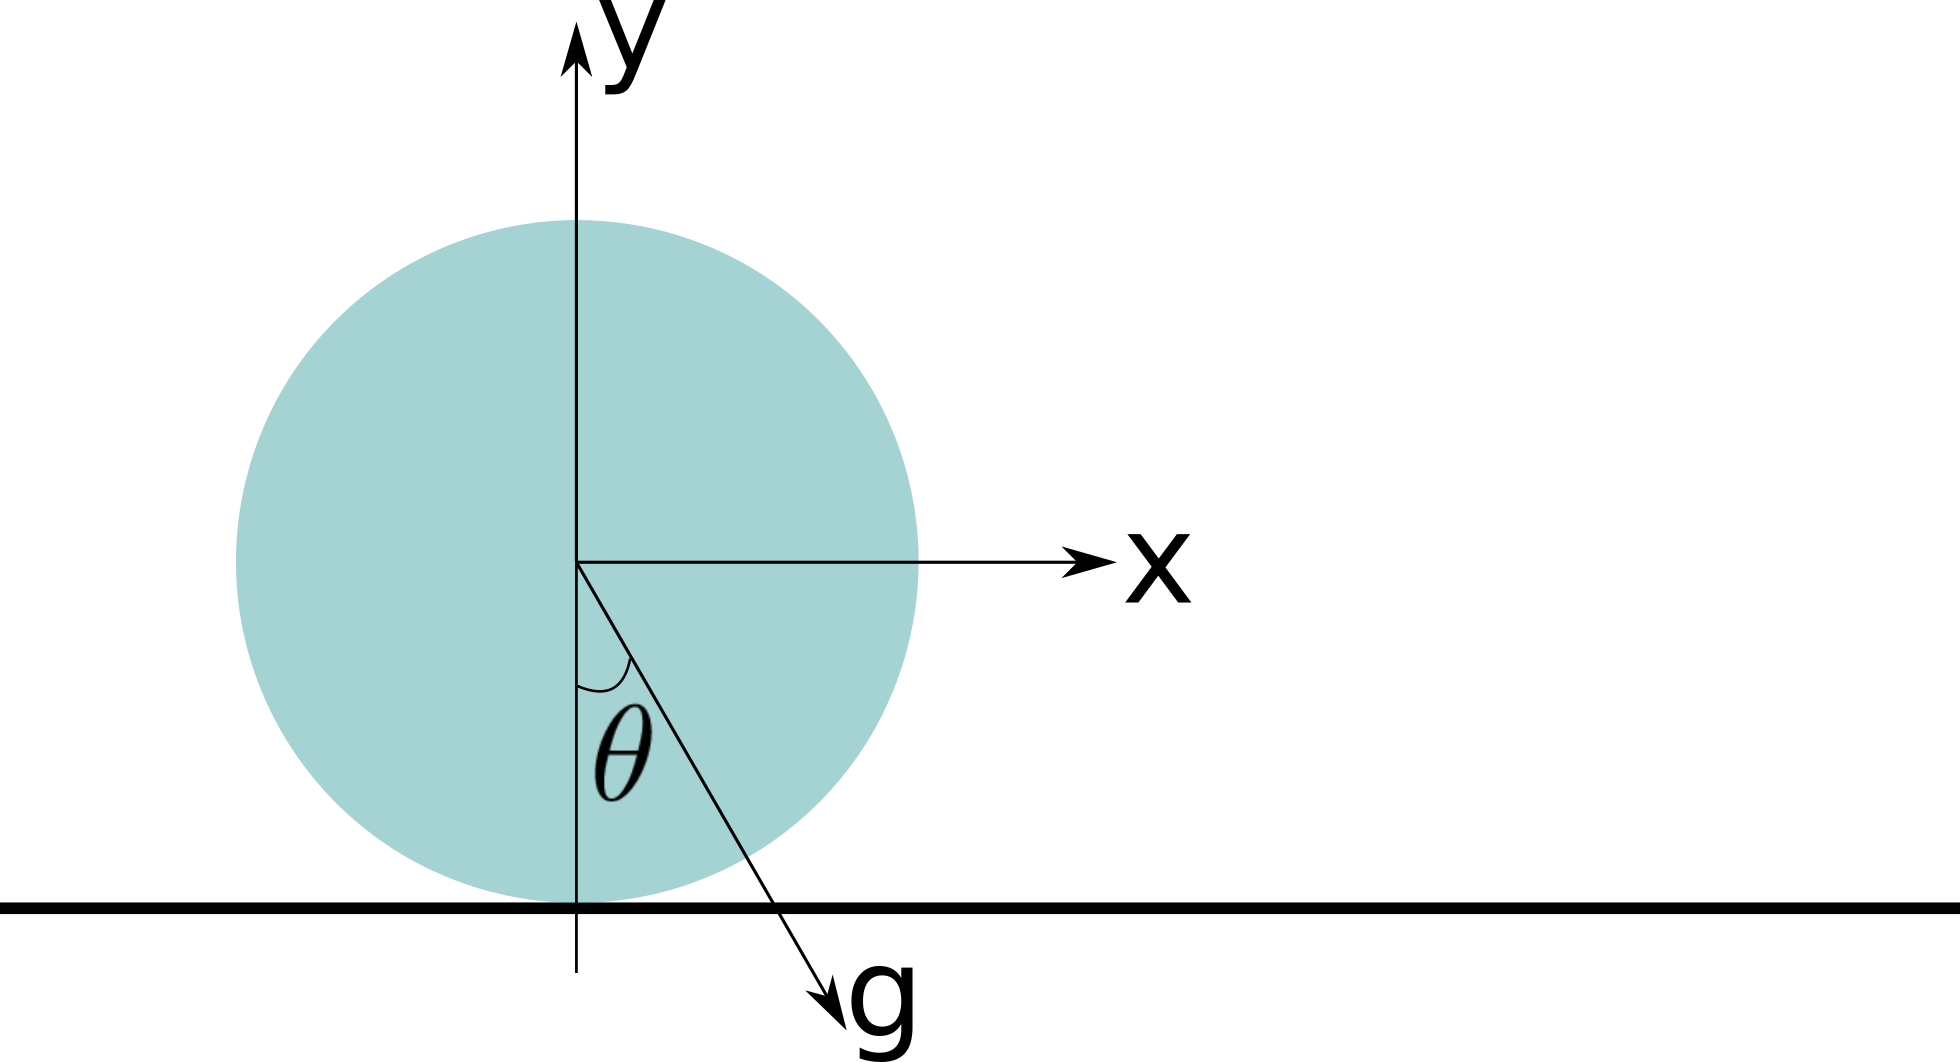
\includegraphics[width=1.0\textwidth]{images/rfc/images/de_2021_cylinder_rolling_on_an_inclined_plane/schematic_2}
    \subcaption{}\label{fig:circular-body:schematic-2}
  \end{subfigure}
  \caption{A (a) physical and (b) computational model of the rolling cylinder on a
    plane inclined at an angle $\theta$.}
\label{fig:circular-body-schematic}
\end{figure}
\begin{table}[!ht]
  \centering
  \begin{tabular}[!ht]{ll}
    \toprule
    Quantity & Values\\
    \midrule
    $\rho$, density & $2700$ kg\,m\textsuperscript{-3} \\
    $\mu$, friction coefficient & $0.3$ \& $0.6$ \\
    Time of simulation & $0.6$ s \\
    Resolution, $\delta x$ & $0.0025$ m\\
    Smoothing length factor, $h/\Delta x$ & 1\\
    gravity $[g_x, g_y, g_z]$ & $[g\,\sin(\theta), g\,\cos(\theta), 0.0]$\\
    $k_r$, Repulsive stiffness coefficient & $1e7$ \\
    $k_f$, Repulsive stiffness coefficient & $1e5$ \\
    $\alpha_{damp}$ & 0.\\
    \bottomrule
  \end{tabular}
  \caption{Material properties and numerical parameters used for the rolling
    of cylinder on an inclined surface.}%
  \label{tab:circular-body-rolling-params}
\end{table}

\Cref{fig:cylinder-xcom-vs-time} depicts the variation of center of mass of
the cylinder with time for friction coefficients $0.3$ and $0.6$,
respectively. From the \cref{fig:cylinder-xcom-vs-time} we can see that the
current solver matches well with the analytical solution.
\begin{figure}[!htpb]
  \centering
  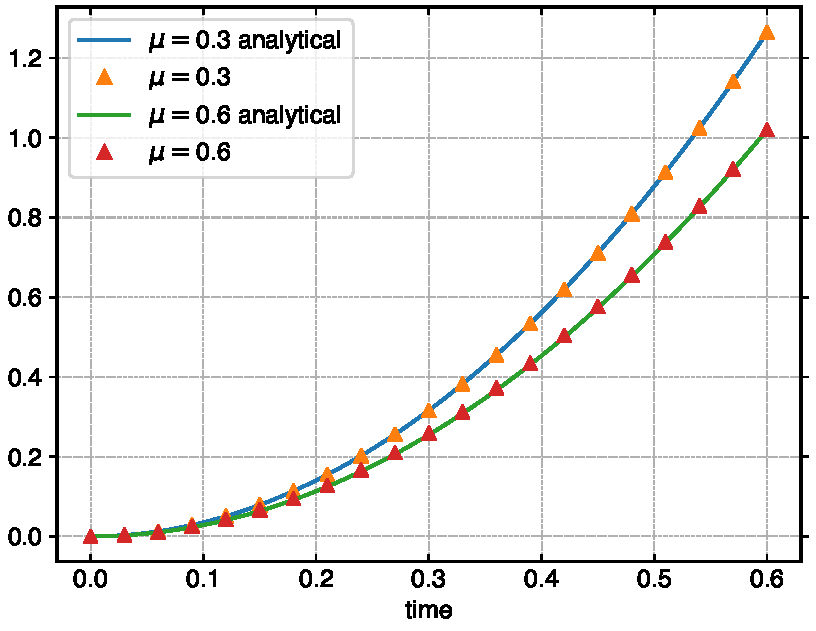
\includegraphics[width=0.4\textwidth]{figures/rfc/figures/de_2021_cylinder_rolling_on_an_inclined_plane_2d/xcom_vs_time}
  \caption{x-component of center of mass variation with time for a cylinder
    rolling down an inclined plane.}
\label{fig:cylinder-xcom-vs-time}
\end{figure}


\FloatBarrier%
\subsection{Rigid body sliding down an inclined plane}
\label{sec:rigid-body-sliding}
In this test case, free sliding of a rigid cube on a frictional inclined plane
is studied. The frictional part of the current solver is validated through this
test. The velocity of the center of mass of the cube is compared against the
analytical solution for quantitative validation. The schematic is shown is
\cref{fig:rigid_body_sliding}.
\begin{figure}[!htpb]
  \centering
  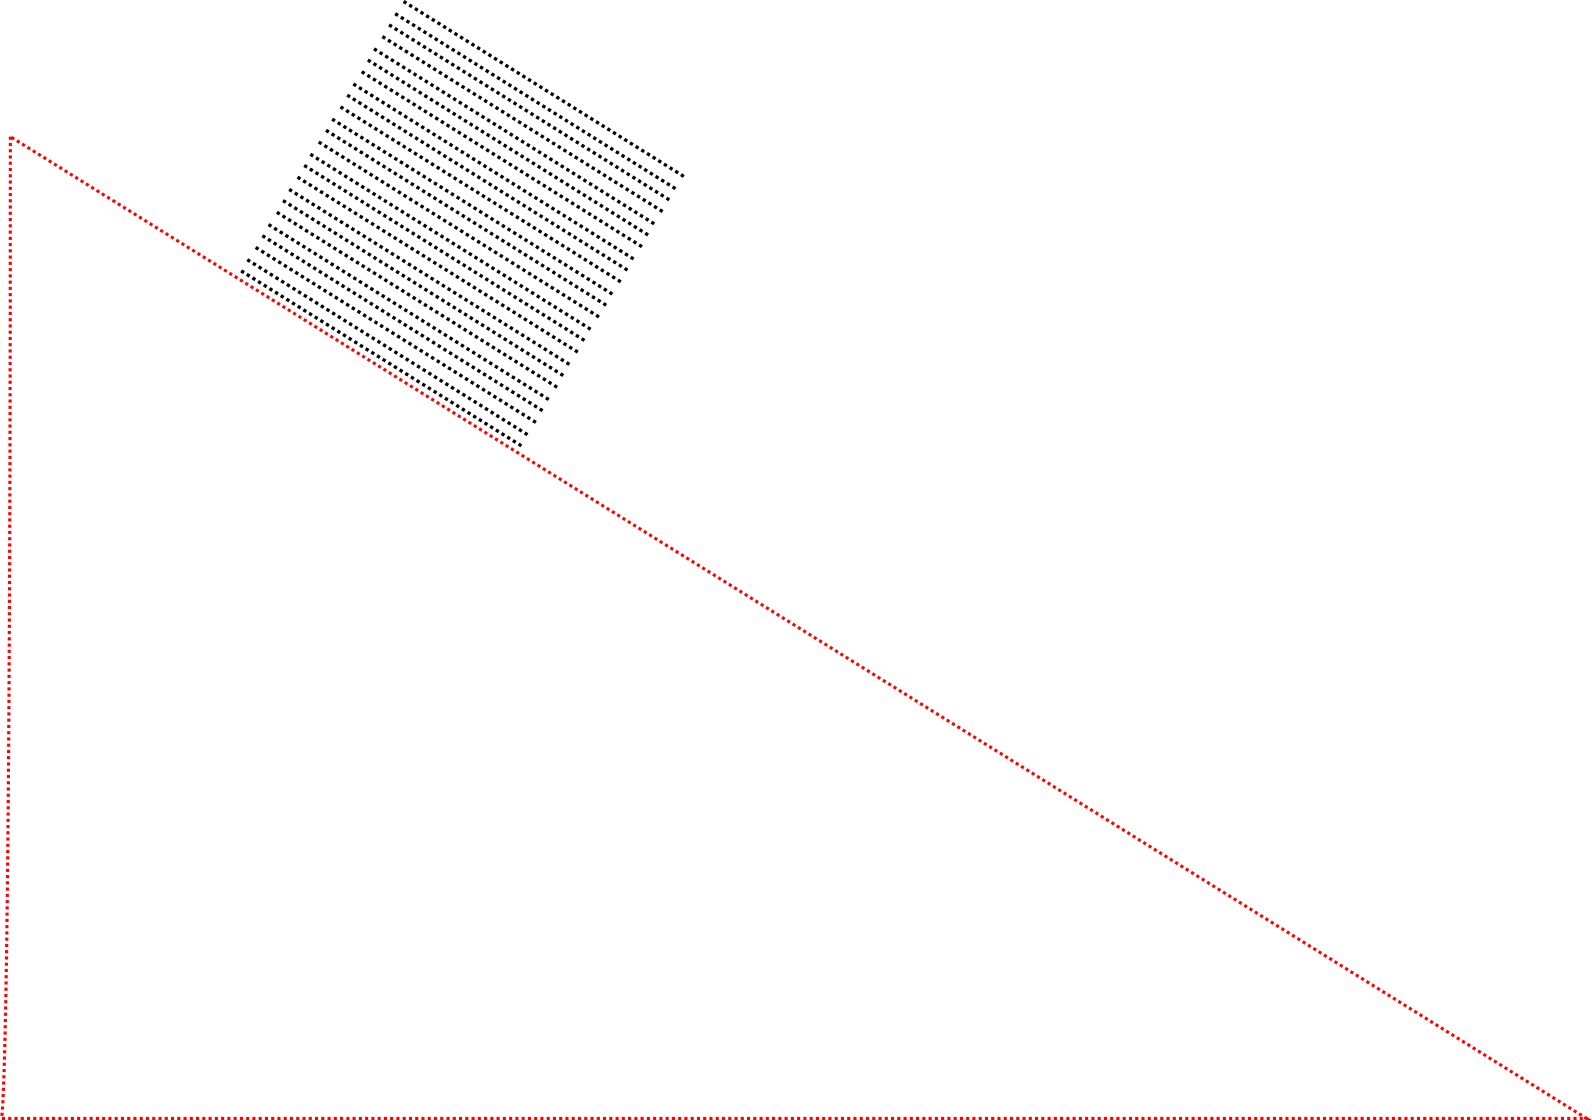
\includegraphics[width=0.4\textwidth]{images/rfc/images/rigid_body_sliding/schematic}
  \caption{Schematic of a square body sliding down an inclined plane under gravity.}
\label{fig:rigid_body_sliding}
\end{figure}
The rigid body of length $0.1$ m, height $0.1$ m, is allowed to slide on a
frictional surface which is at an angle $\frac{\pi}{3}$. A density of $2000$
kg\,m\textsuperscript{-3} is used for the body. Other numerical parameters, such
as the repulsive spring stiffness $k_r=3.0 \times 10^{5}$ $N/m$ and tangential
spring stiffness $k_t=3.0 \times 10^{5}$ $N/m$ is chosen, respectively. A
particle spacing of $0.001$ m is considered, resulting in $120$ particles in
rigid body discretization. From the analytical solution, the evolution of
velocity is given by,
\begin{equation}
  \label{eq:ce}
  \ten{v}(t) = (\mu \teng{g} \sin (\theta) - \teng{g} \cos (\theta)) t.
\end{equation}

We have considered three different friction coefficients, $\mu=0.2$,
$\mu=0.3$, and $\mu=0.6$. From the analytical solution, when the friction
coefficient is greater than $\tan(\frac{\pi}{3})$, we have no slip condition
and the body doesn't slide.

% \subsubsection{2D sliding}
% \label{sec:results-2d-sliding}
\Cref{fig:mohseni-2021-sliding-2d} shows the snapshots of the rigid body at
three time instants. From \cref{fig:mohseni-2021-sliding-2d} we can see that
the the body is freely sliding with out having any oscillations or unphysical
jumping off the inclined wall. This is because of the new surface aware
contact model as force is not computed by considering the wall as spherical
\begin{figure}[!htpb]
  \centering
  \begin{subfigure}{0.48\textwidth}
    \centering
    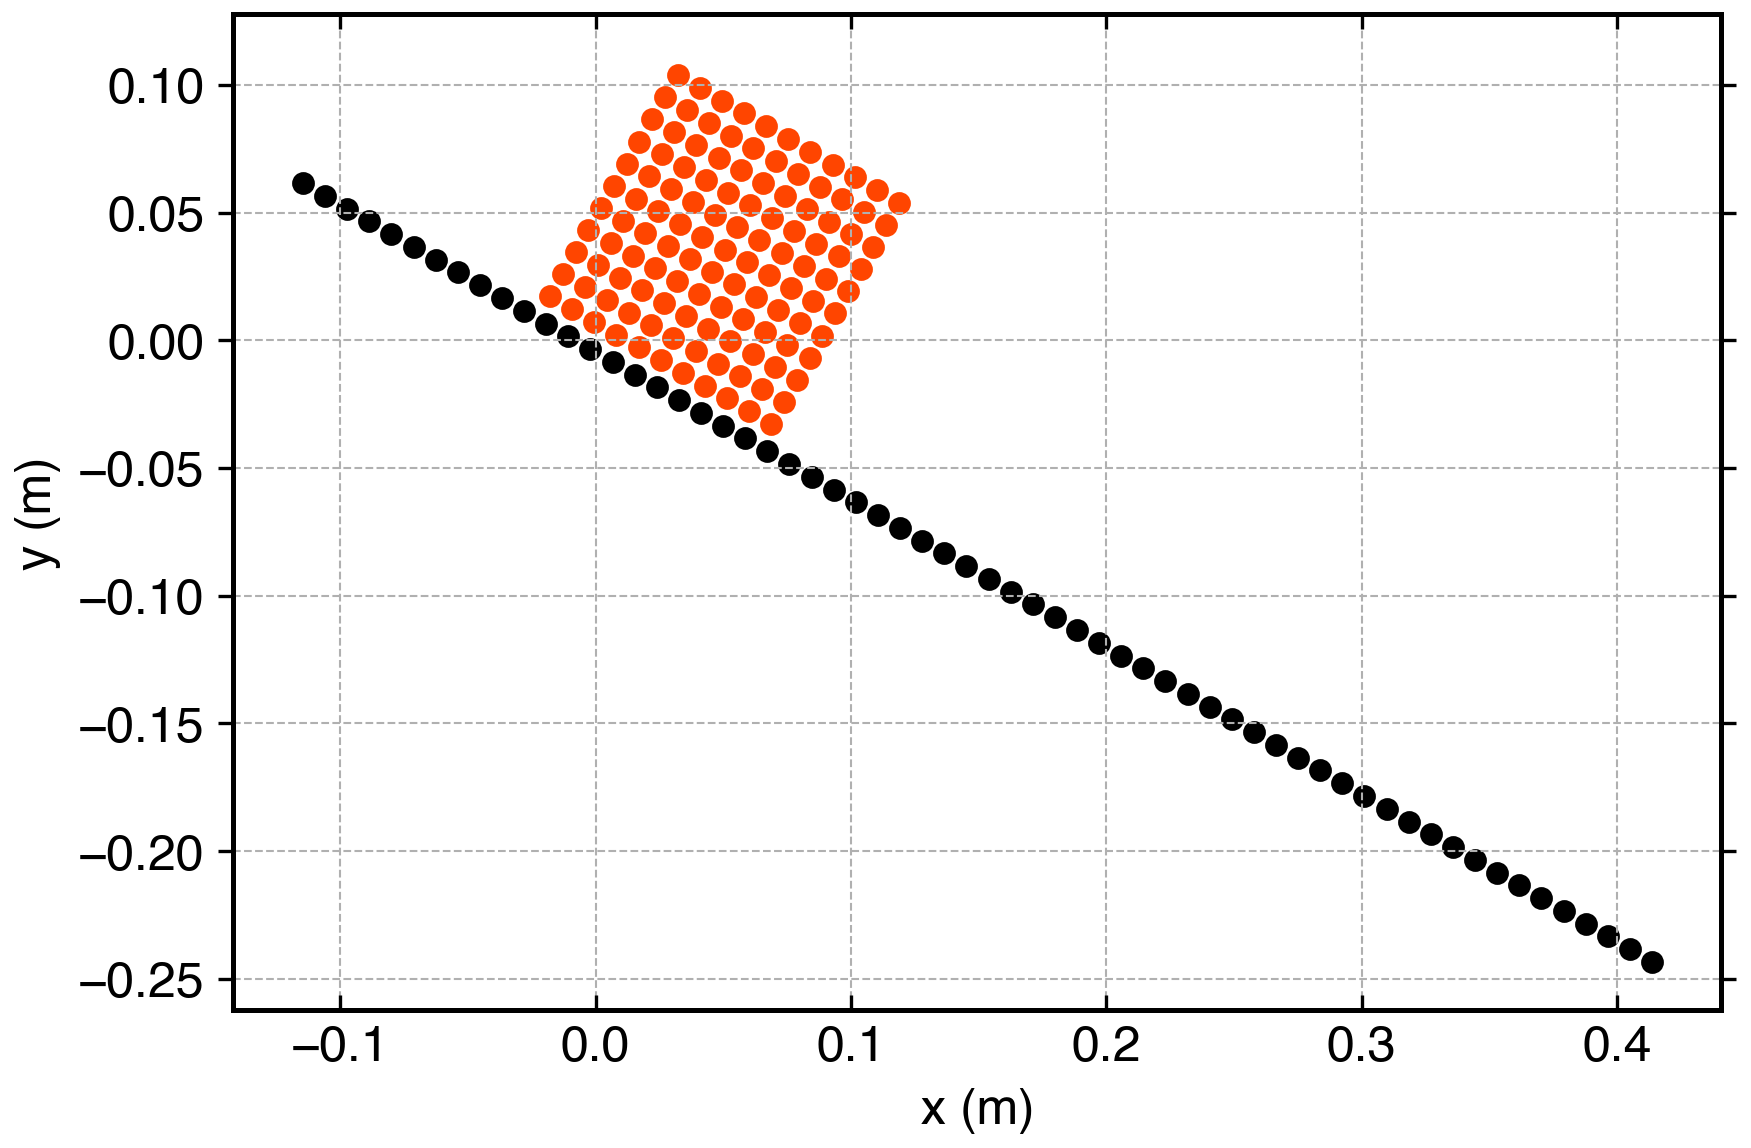
\includegraphics[width=1.0\textwidth]{figures/rfc/figures/mohseni_2021_free_sliding_on_a_slope_2d/fric_coeff_0_2/time0}
    \subcaption{t = $0$ s}\label{fig:passing-0}
  \end{subfigure}
  %
  \begin{subfigure}{0.48\textwidth}
    \centering
    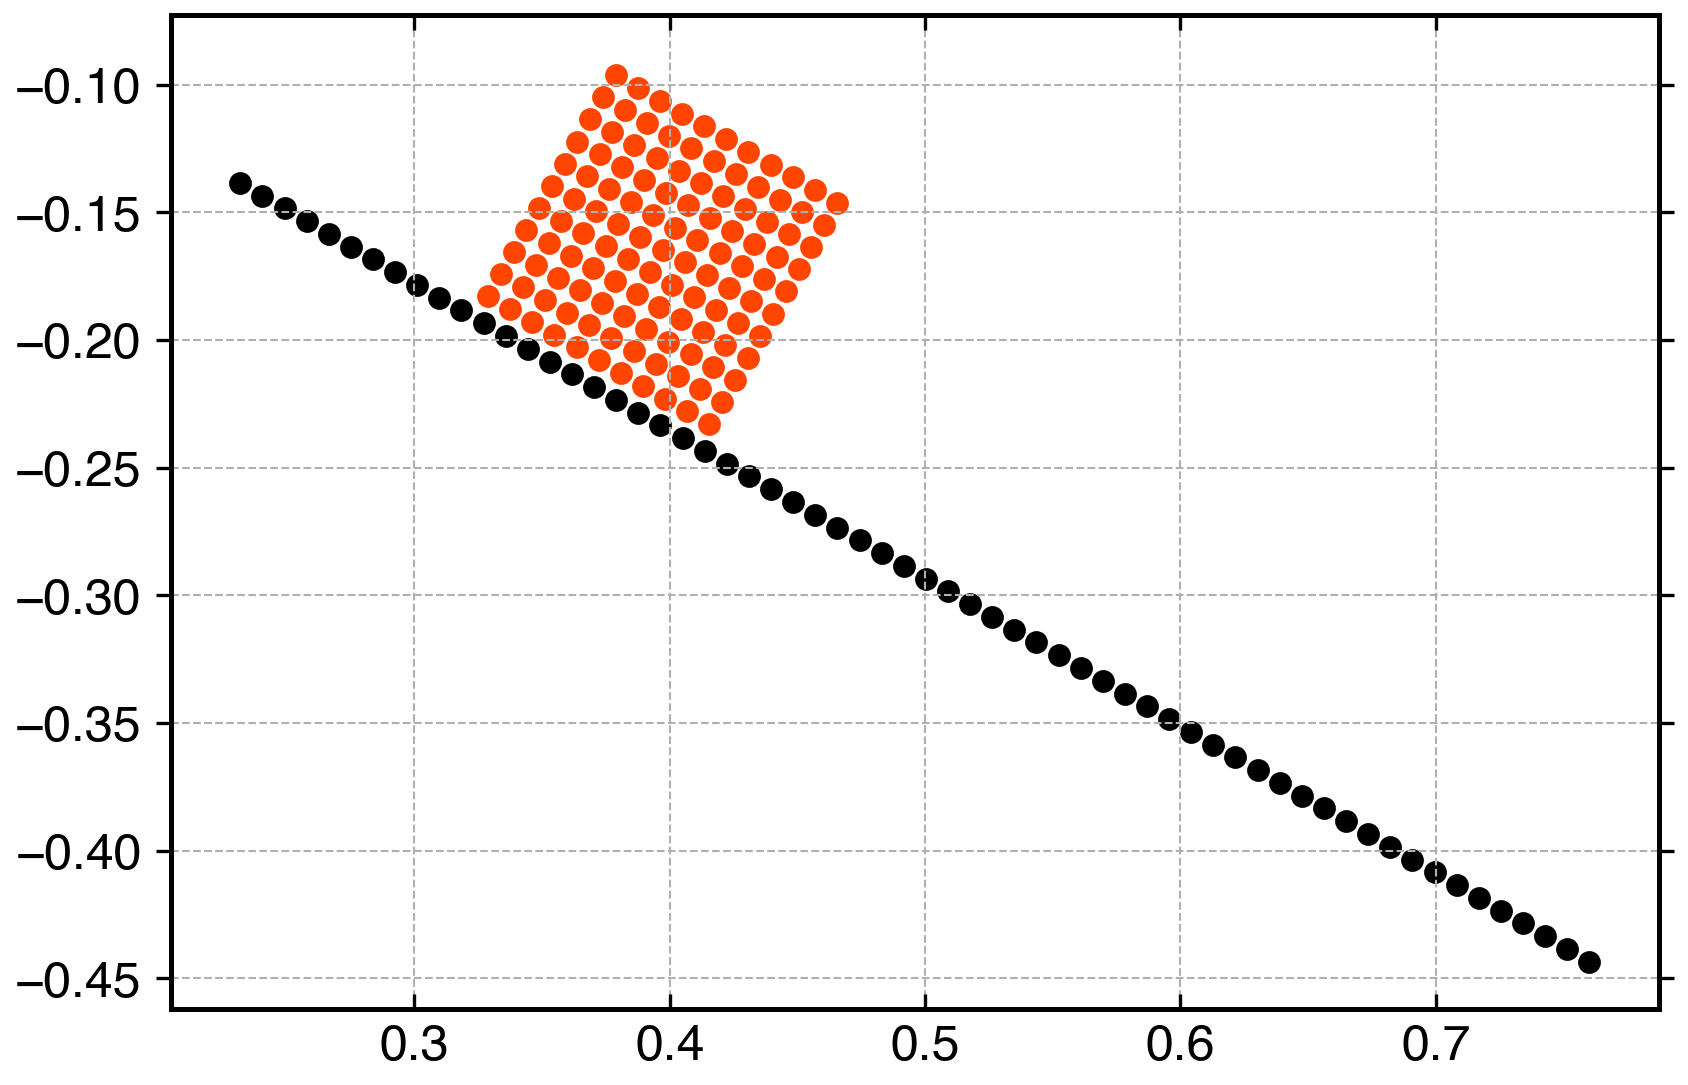
\includegraphics[width=1.0\textwidth]{figures/rfc/figures/mohseni_2021_free_sliding_on_a_slope_2d/fric_coeff_0_2/time1}
    \subcaption{t = $0.5$ s}\label{fig:passing-1}
  \end{subfigure}

  \begin{subfigure}{0.48\textwidth}
    \centering
    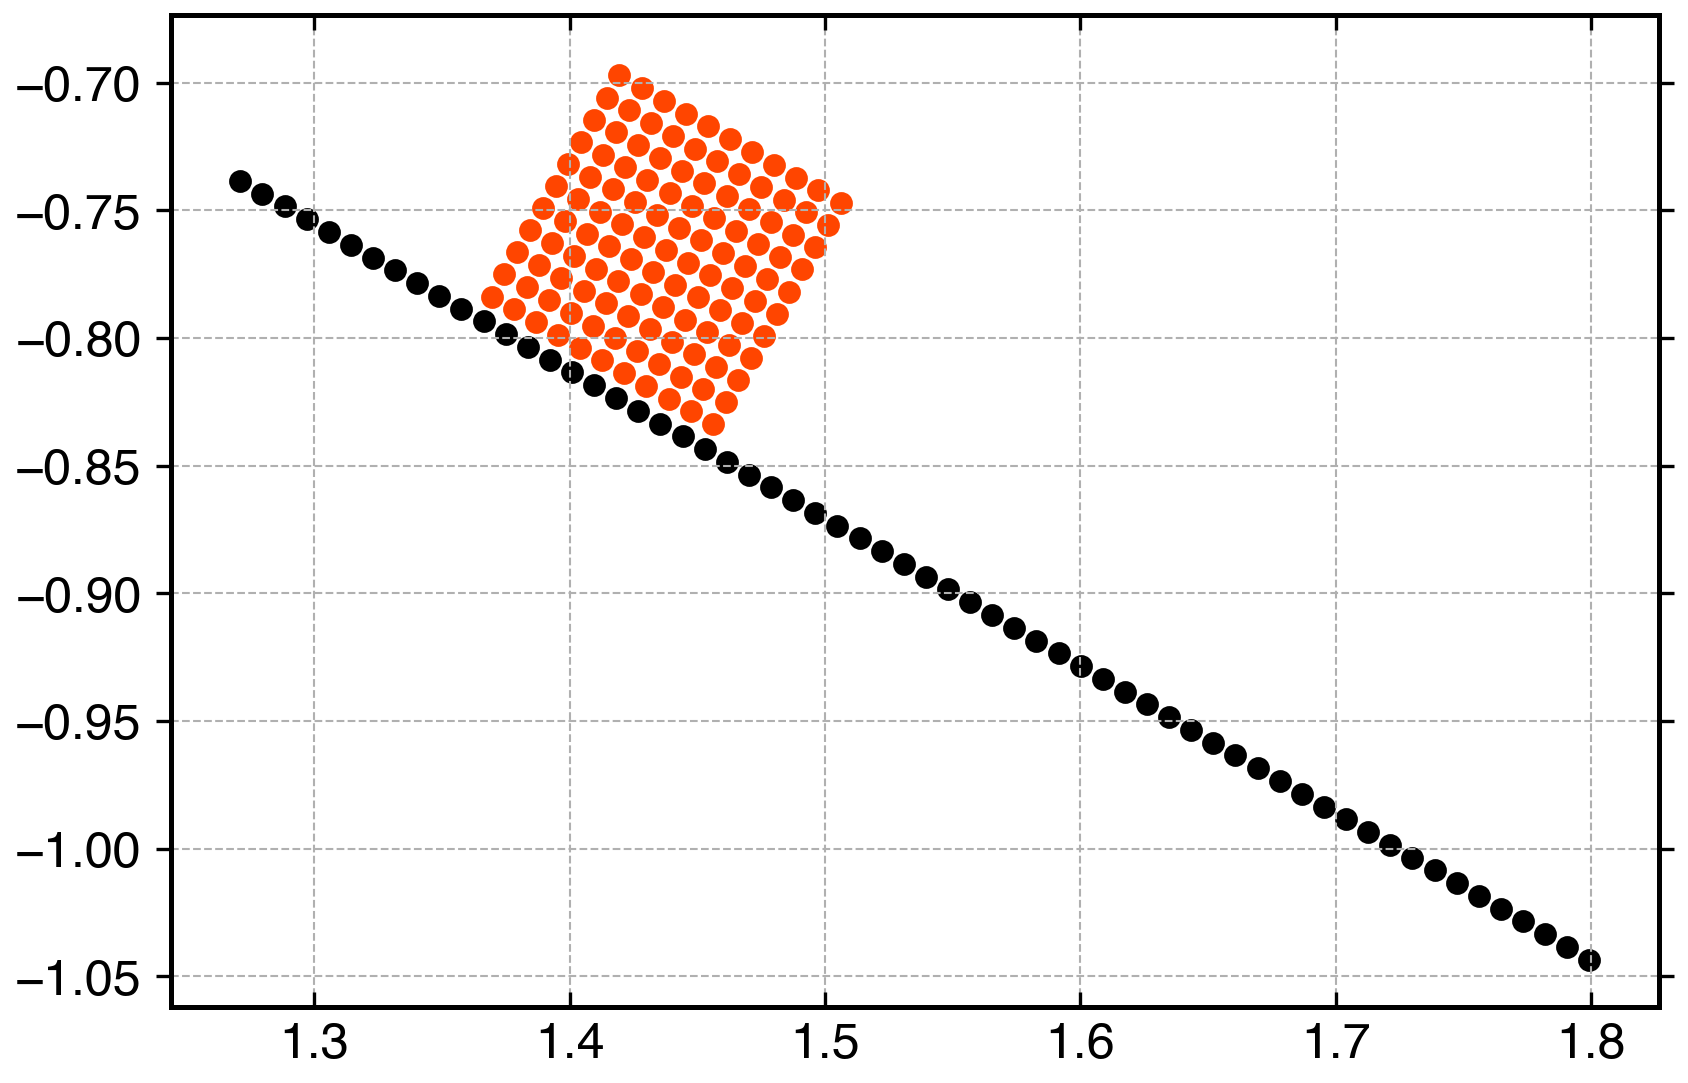
\includegraphics[width=1.0\textwidth]{figures/rfc/figures/mohseni_2021_free_sliding_on_a_slope_2d/fric_coeff_0_2/time2}
    \subcaption{t = $1$ s}\label{fig:passing-2}
  \end{subfigure}
  \caption{Snapshots of rigid body sliding down an inclined plane with a
    friction coefficient of $0.2$.}
\label{fig:mohseni-2021-sliding-2d}
\end{figure}
particles but by ensemble of an overlap. The snapshots correspond to a
friction coefficient of $0.2$.
\Cref{fig:results-solid-sliding-velocity-vs-time-2d} shows a evolution of
velocity of the center of mass of the rigid body for different frictional
coefficients against the analytical solution. From
\cref{fig:results-solid-sliding-velocity-vs-time-2d} we can see that the current
solver has an excellent match with the analytical solution and covers all the
regimes of the sliding case.
\begin{figure}[!htpb]
  \centering
  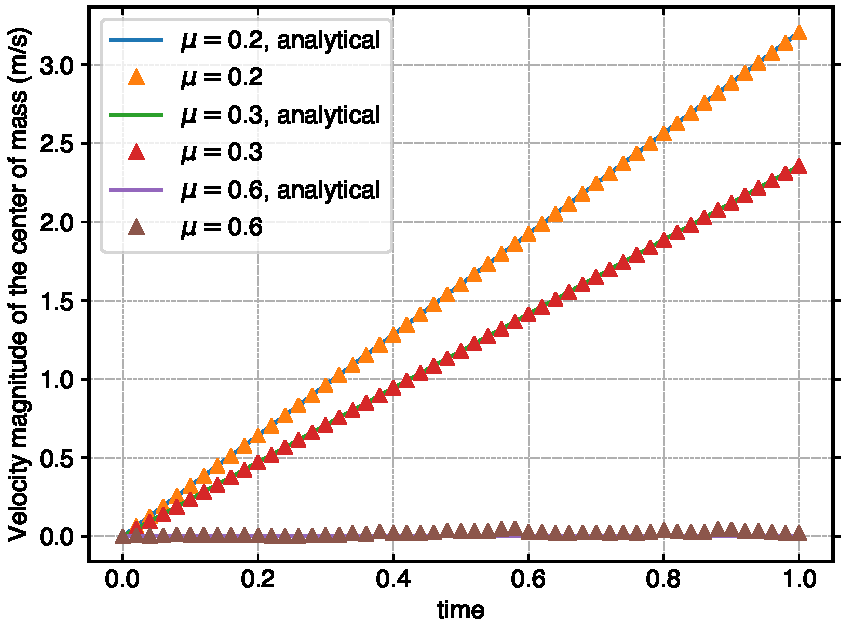
\includegraphics[width=0.5\textwidth]{figures/rfc/figures/mohseni_2021_free_sliding_on_a_slope_2d/velocity_vs_time}
  \caption{Variation of the velocity of the rigid body with time for different
    friction coefficients. Present result is compared against the analytical
    result.}
\label{fig:results-solid-sliding-velocity-vs-time-2d}
\end{figure}

\subsubsection{3D sliding}
\label{sec:results-3d-sliding}

\Cref{fig:mohseni-2021-sliding-3d} shows the snapshots of the rigid body at
three time instants for a 3D sliding case. From
\cref{fig:mohseni-2021-sliding-3d} we can see that the the body is freely
sliding with out having any oscillations or unphysical jumping off the inclined
wall. The snapshots correspond to a friction coefficient of $0.4$.
\Cref{fig:results-solid-sliding-velocity-vs-time-3d} shows a evolution of
velocity of the center of mass of the rigid body for different frictional
coefficients against the analytical solution. From
\Cref{fig:results-solid-sliding-velocity-vs-time-3d} we can see that the current
solver has an excellent match with the analytical solution and covers all the
regimes of the sliding case for a 3D case.
\begin{figure}[!htpb]
  \centering
  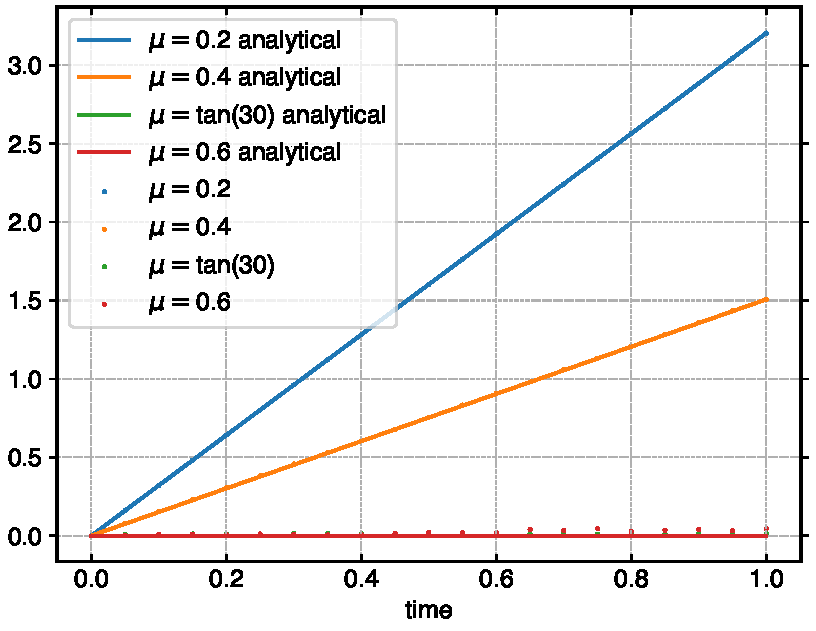
\includegraphics[width=0.6\textwidth]{figures/rfc/figures/mohseni_2021_free_sliding_on_a_slope_3d/velocity_vs_time}
  \caption{A 3D case - Variation of the velocity of the rigid body with time for different
    friction coefficients. Present result is compared against the analytical
    result.}
\label{fig:results-solid-sliding-velocity-vs-time-3d}
\end{figure}

\begin{figure}[!htpb]
  \centering
  \begin{subfigure}{0.48\textwidth}
    \centering
    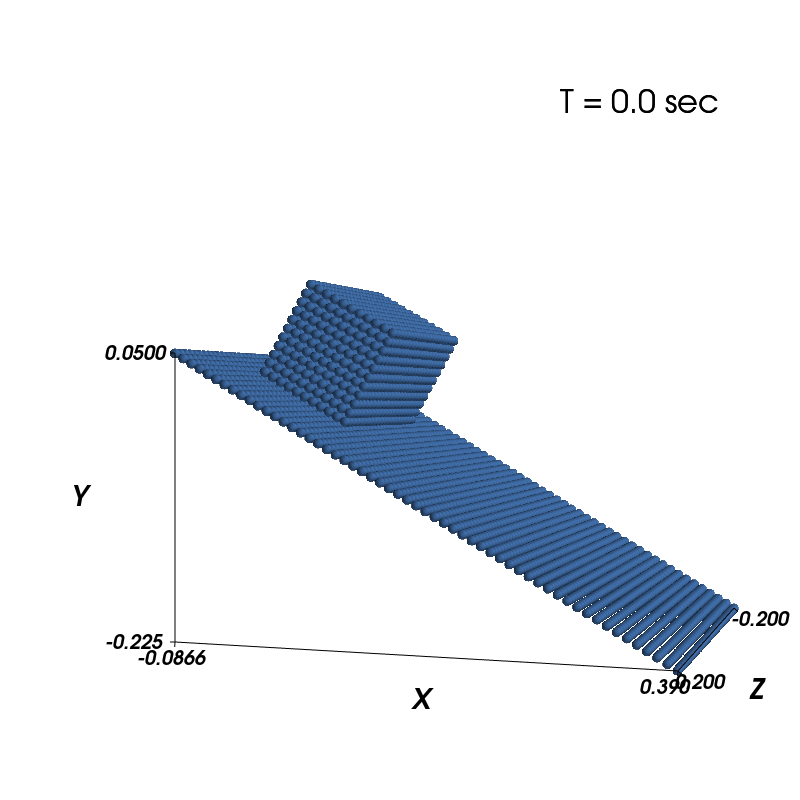
\includegraphics[width=1.0\textwidth]{figures/rfc/figures/mohseni_2021_free_sliding_on_a_slope_3d/fric_coeff_0_2/time0}
    \subcaption{t = $0$ sec}\label{fig:passing-0}
  \end{subfigure}
  %
  \begin{subfigure}{0.48\textwidth}
    \centering
    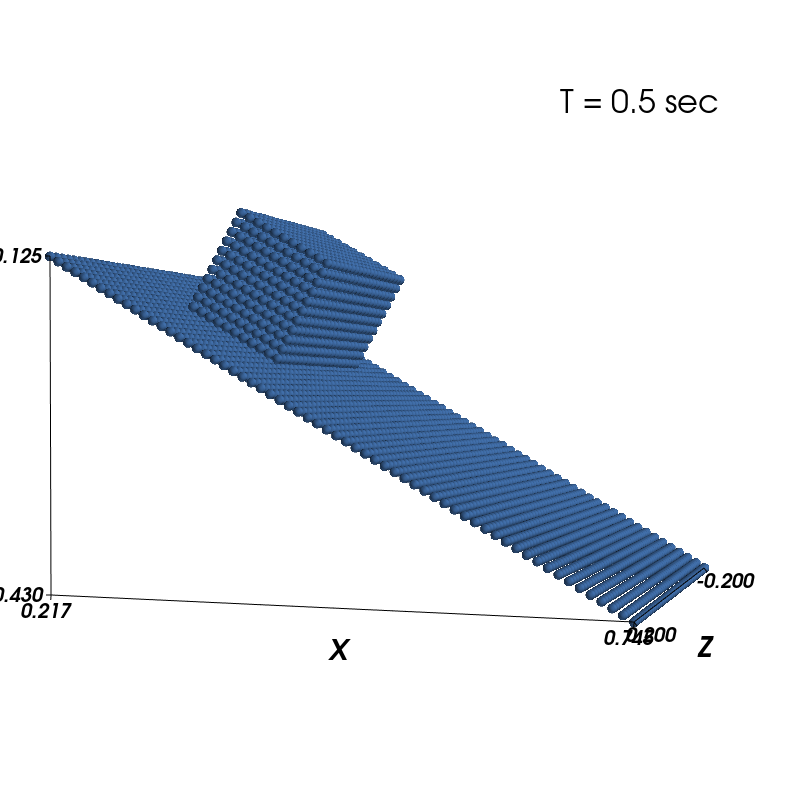
\includegraphics[width=1.0\textwidth]{figures/rfc/figures/mohseni_2021_free_sliding_on_a_slope_3d/fric_coeff_0_2/time1}
    \subcaption{t = $0.5$ sec}\label{fig:passing-1}
  \end{subfigure}

  \begin{subfigure}{0.48\textwidth}
    \centering
    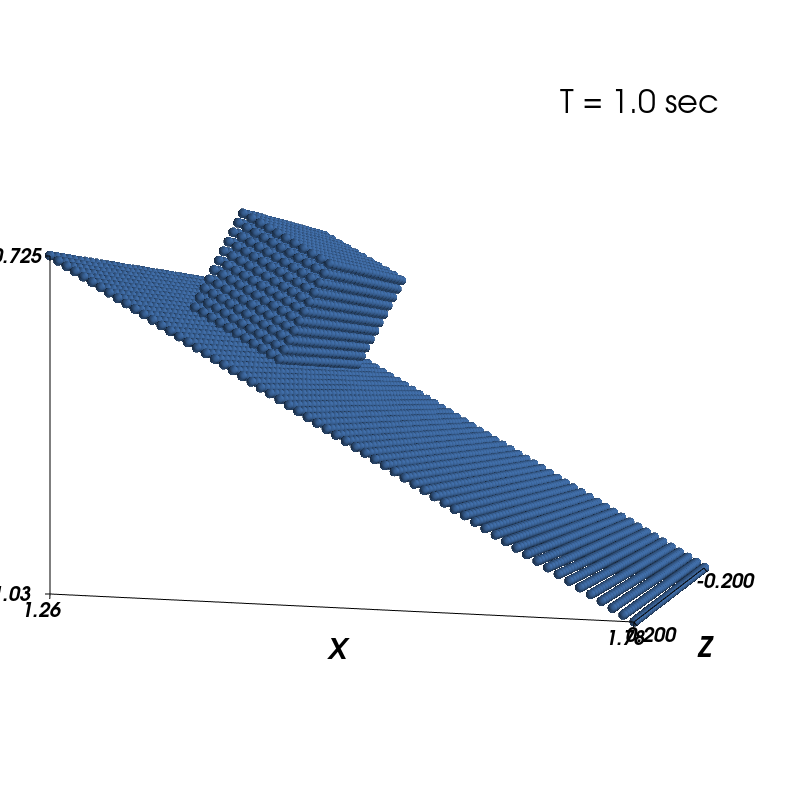
\includegraphics[width=1.0\textwidth]{figures/rfc/figures/mohseni_2021_free_sliding_on_a_slope_3d/fric_coeff_0_2/time2}
    \subcaption{t = $1.0$ sec}\label{fig:passing-2}
  \end{subfigure}
  \caption{3D case - Snapshots of rigid body sliding down an inclined plane with a
    friction coefficient of $0.2$.}
\label{fig:mohseni-2021-sliding-3d}
\end{figure}


\FloatBarrier%
\subsection{Controlled Sliding on a Flat Surface}
\label{sec:controlled-rigid-body-sliding}
A controlled sliding of rigid body on a frictional surface is studied in the
current test case. The schematic of the rigid body as well as the wall is shown
in \cref{fig:schematic-controlled-rigid-body-sliding}. The rigid body is acted
upon by normal ($\ten{F}$) and tangential force ($\ten{T}$), where, force
$\ten{F}$ is applied on top of the body for $1.0$ second, which gradually
increases to $2000$ N till $0.5$ seconds, and stays constant till $1.0$ second.
Once the normal force $\ten{N}$ reaches $2000$ N, we start applying the
tangential force of magnitude $4000$ N, which increases linearly till $1.0$
seconds. The friction coefficient between the body and wall is assumed to be
$0.5$.
\begin{figure}[!htpb]
  \centering
  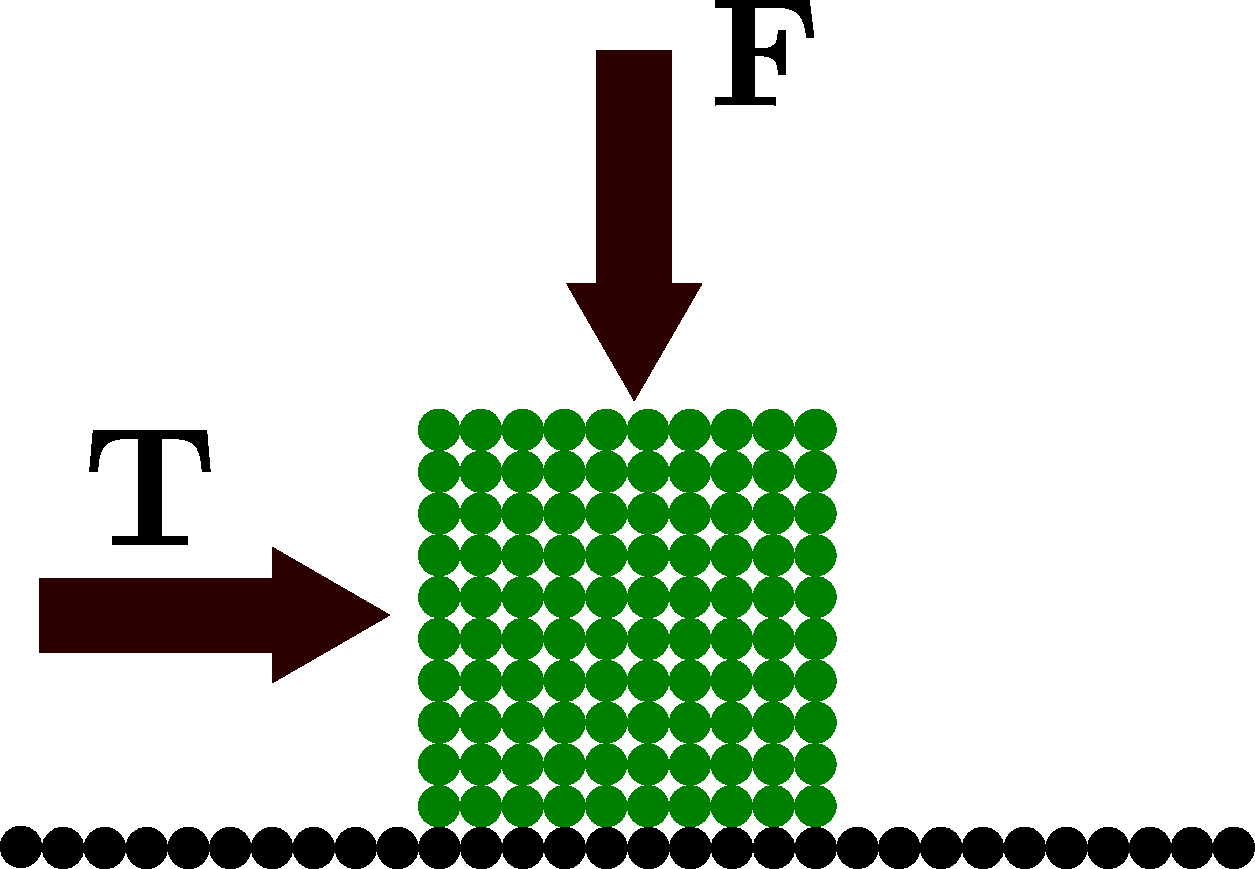
\includegraphics[width=0.5\textwidth]{images/rfc/images/controlled_rigid_body_sliding/schematic}
  \caption{Schematic of the controlled sliding of a rigid body.}
\label{fig:schematic-controlled-rigid-body-sliding}
\end{figure}

\Cref{fig:velocity-vs-time-controlled-sliding} depicts the time histories of
velocity of the center of mass of the rigid body with time, as well as the
variation of applied external normal $\ten{F}$ and tangential $\ten{T}$
forces against the velocity computed using analytical solution.
\begin{figure}[!htpb]
  \centering
  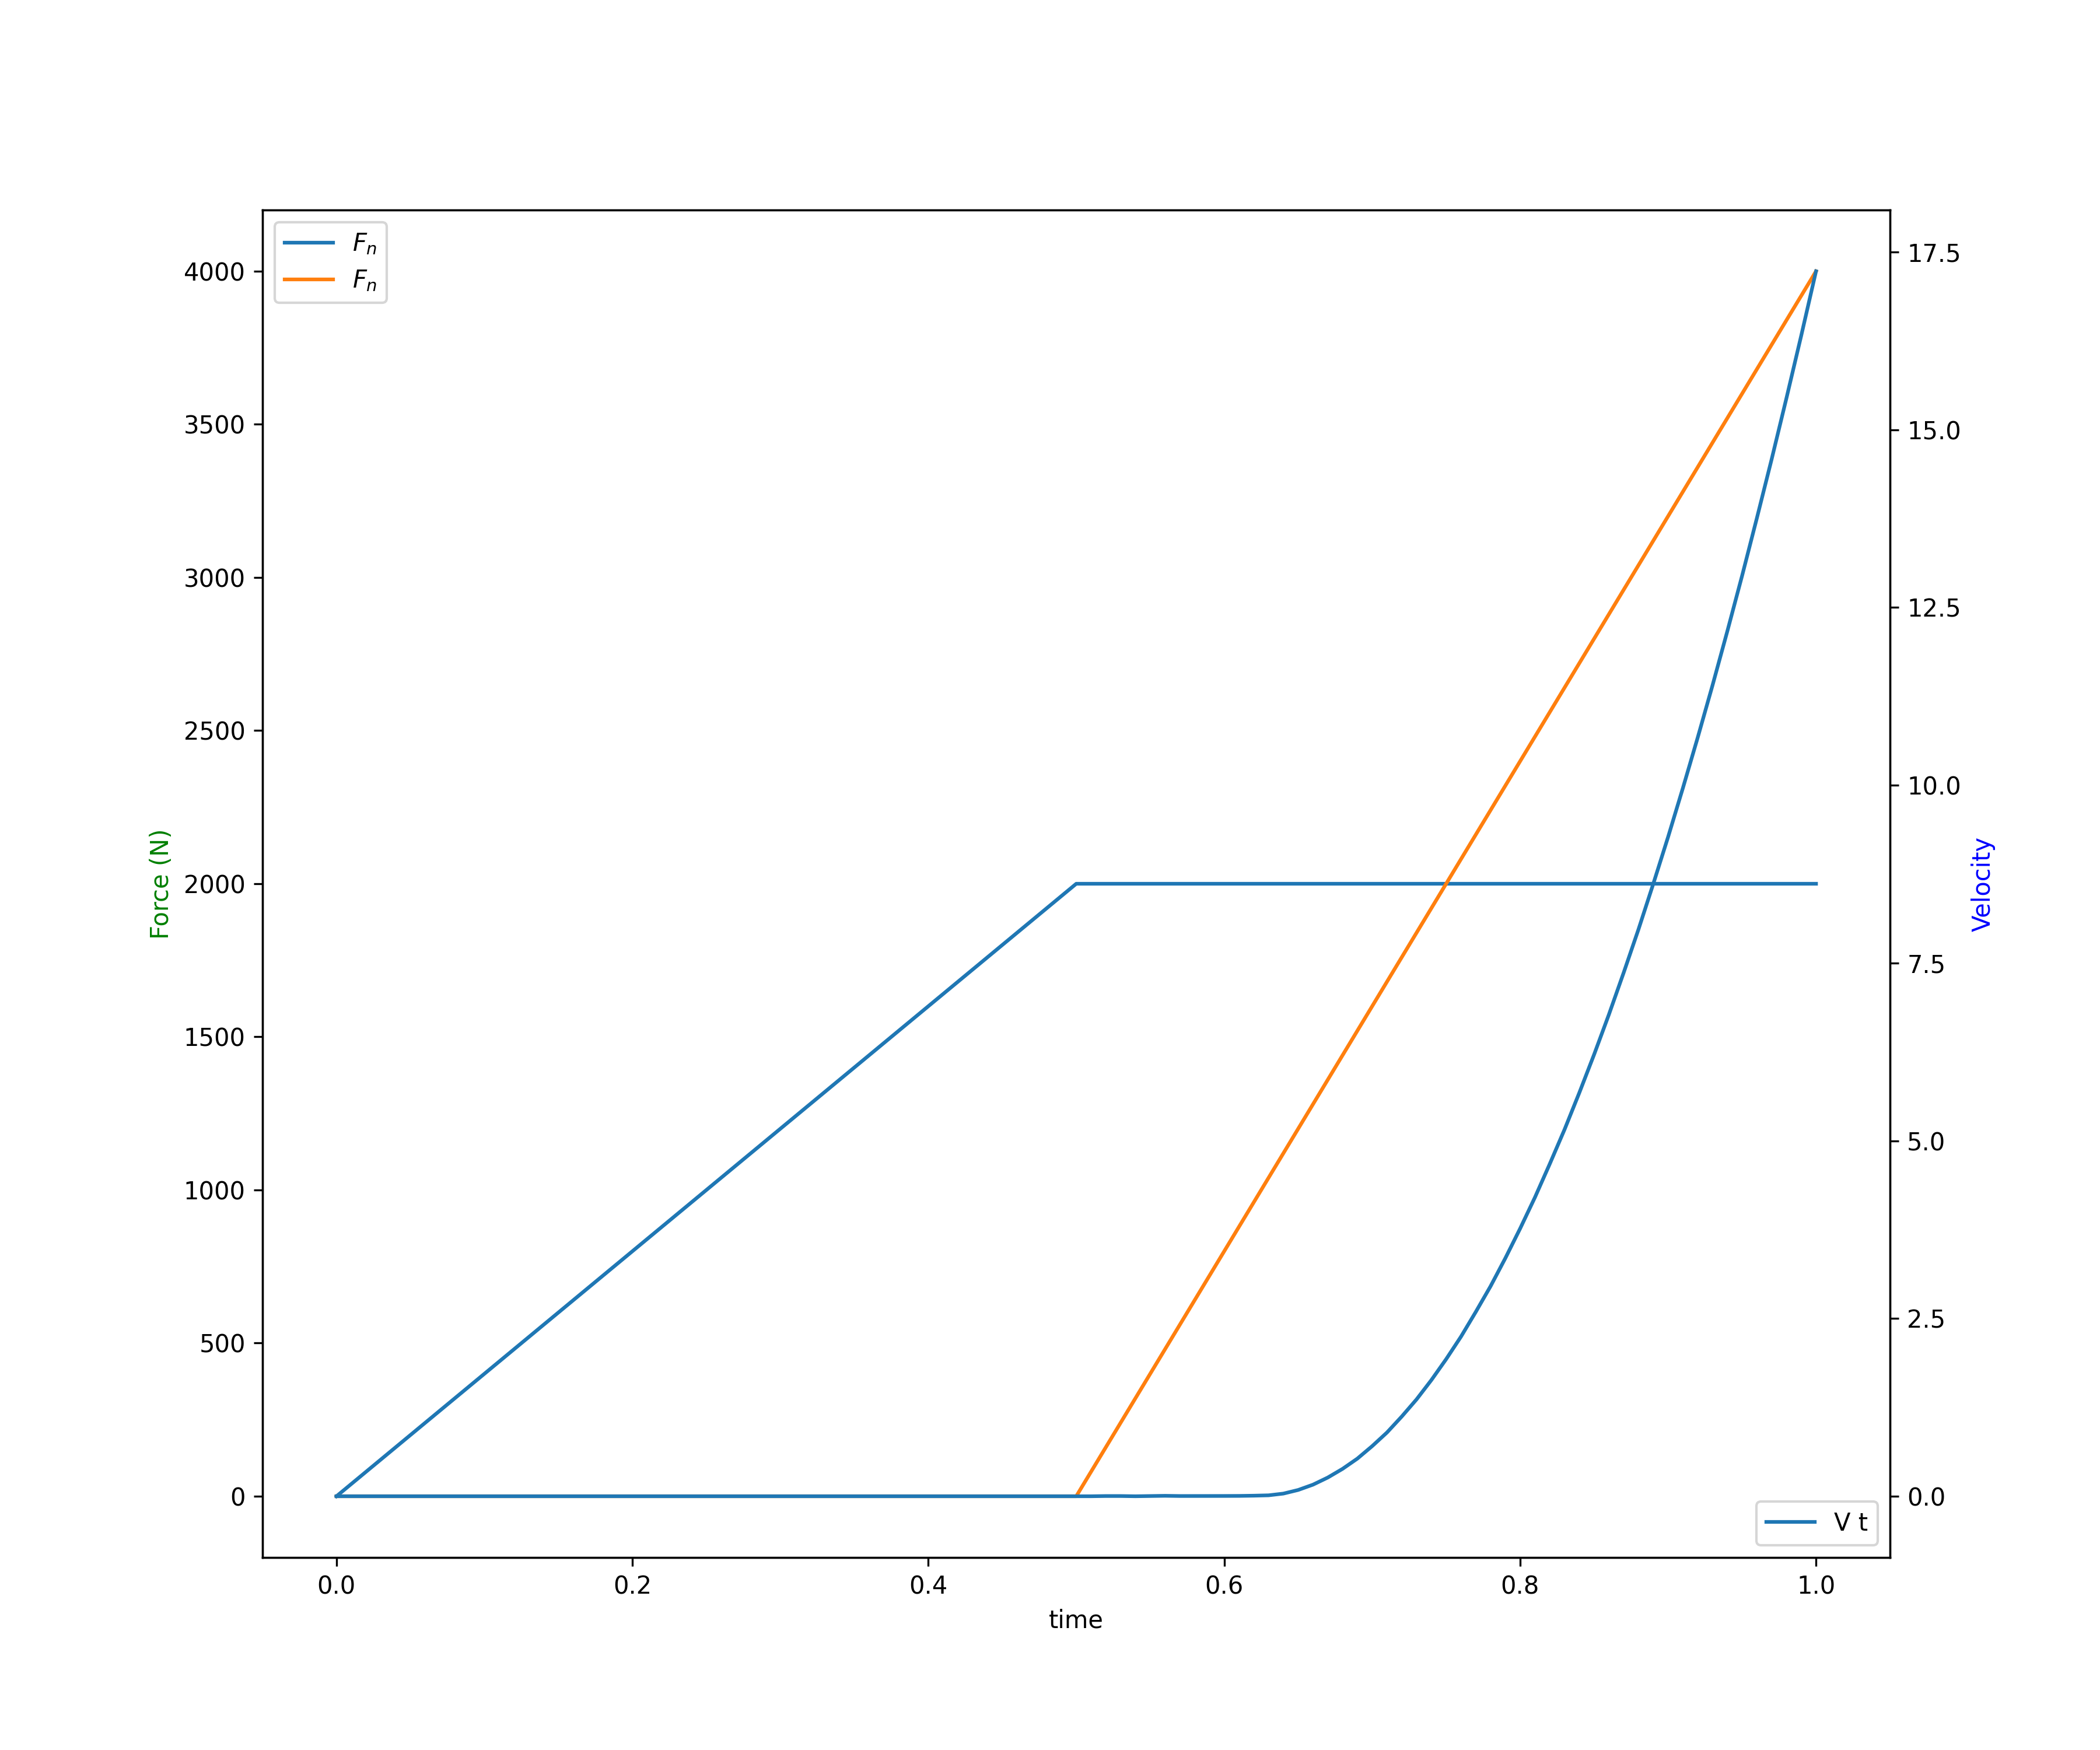
\includegraphics[width=0.7\textwidth]{figures/rfc/figures/mohseni_2021_controlled_sliding_on_a_flat_surface_2d/case_1/force_velocity_vs_t}
  \caption{Force and Velocity vs time curves of the of the controlled rigid slider.}
\label{fig:velocity-vs-time-controlled-sliding}
\end{figure}


% \FloatBarrier
% \subsection{Three bodies colliding}
% \label{sec:three-bodies-colliding}


% \begin{figure}[!htpb]
%   \centering
%   % 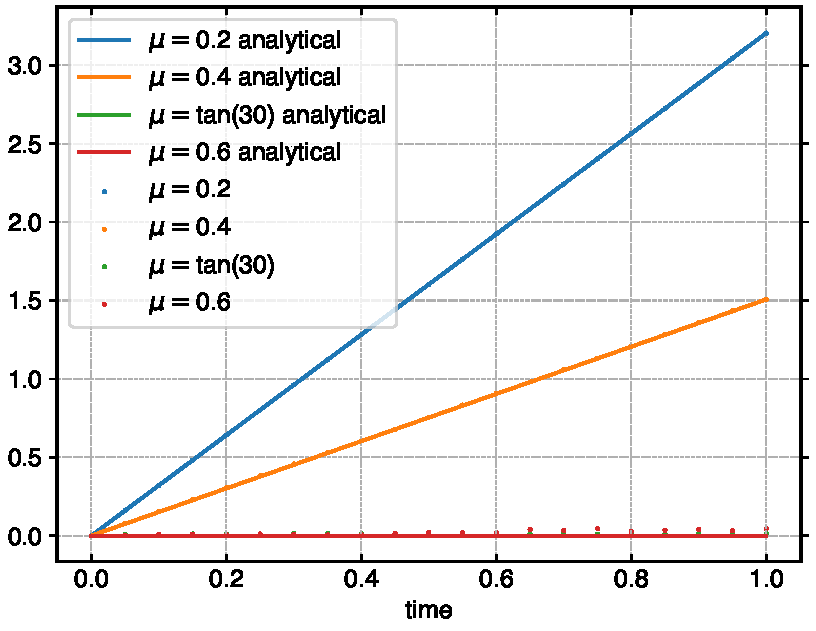
\includegraphics[width=0.4\textwidth]{figures/rfc/figures/mohseni_2021_free_sliding_on_a_slope_3d/velocity_vs_time}
%   \caption{Schematic of the three rigid body colliding}
% \label{fig:schematic-three-rigid-bodies-colliding}
% \end{figure}

% \begin{figure}[!htpb]
%   \centering
%   \begin{subfigure}{0.48\textwidth}
%     \centering
%     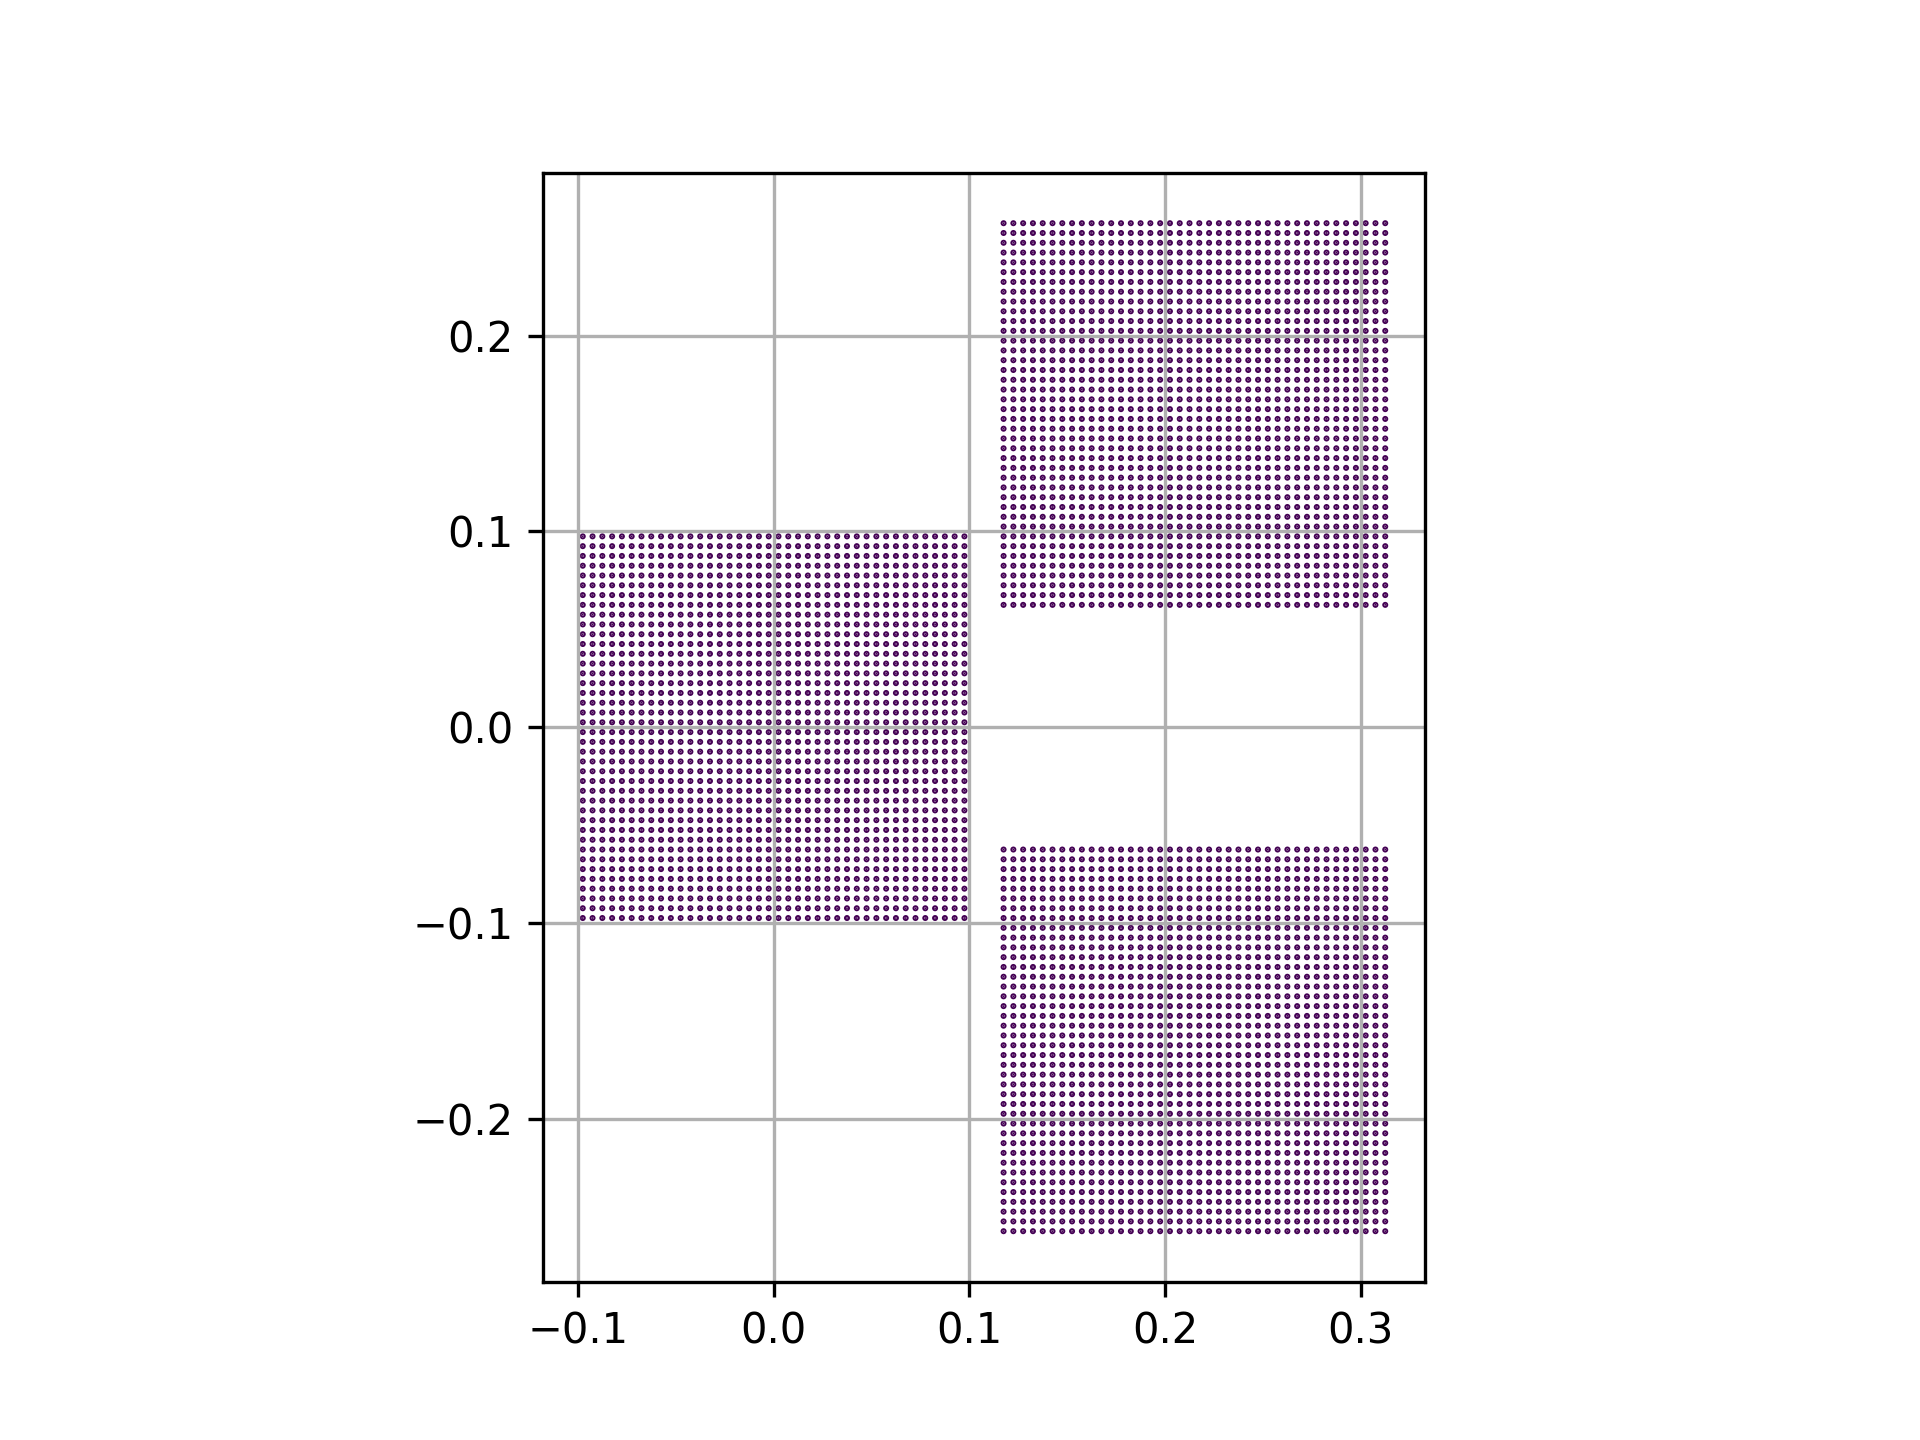
\includegraphics[width=1.0\textwidth]{figures/rfc/figures/amaro_2019_collision_between_three_rigid_cubes/Mohseni_Vyas/time0}
%   \end{subfigure}
%   %
%   \begin{subfigure}{0.48\textwidth}
%     \centering
%     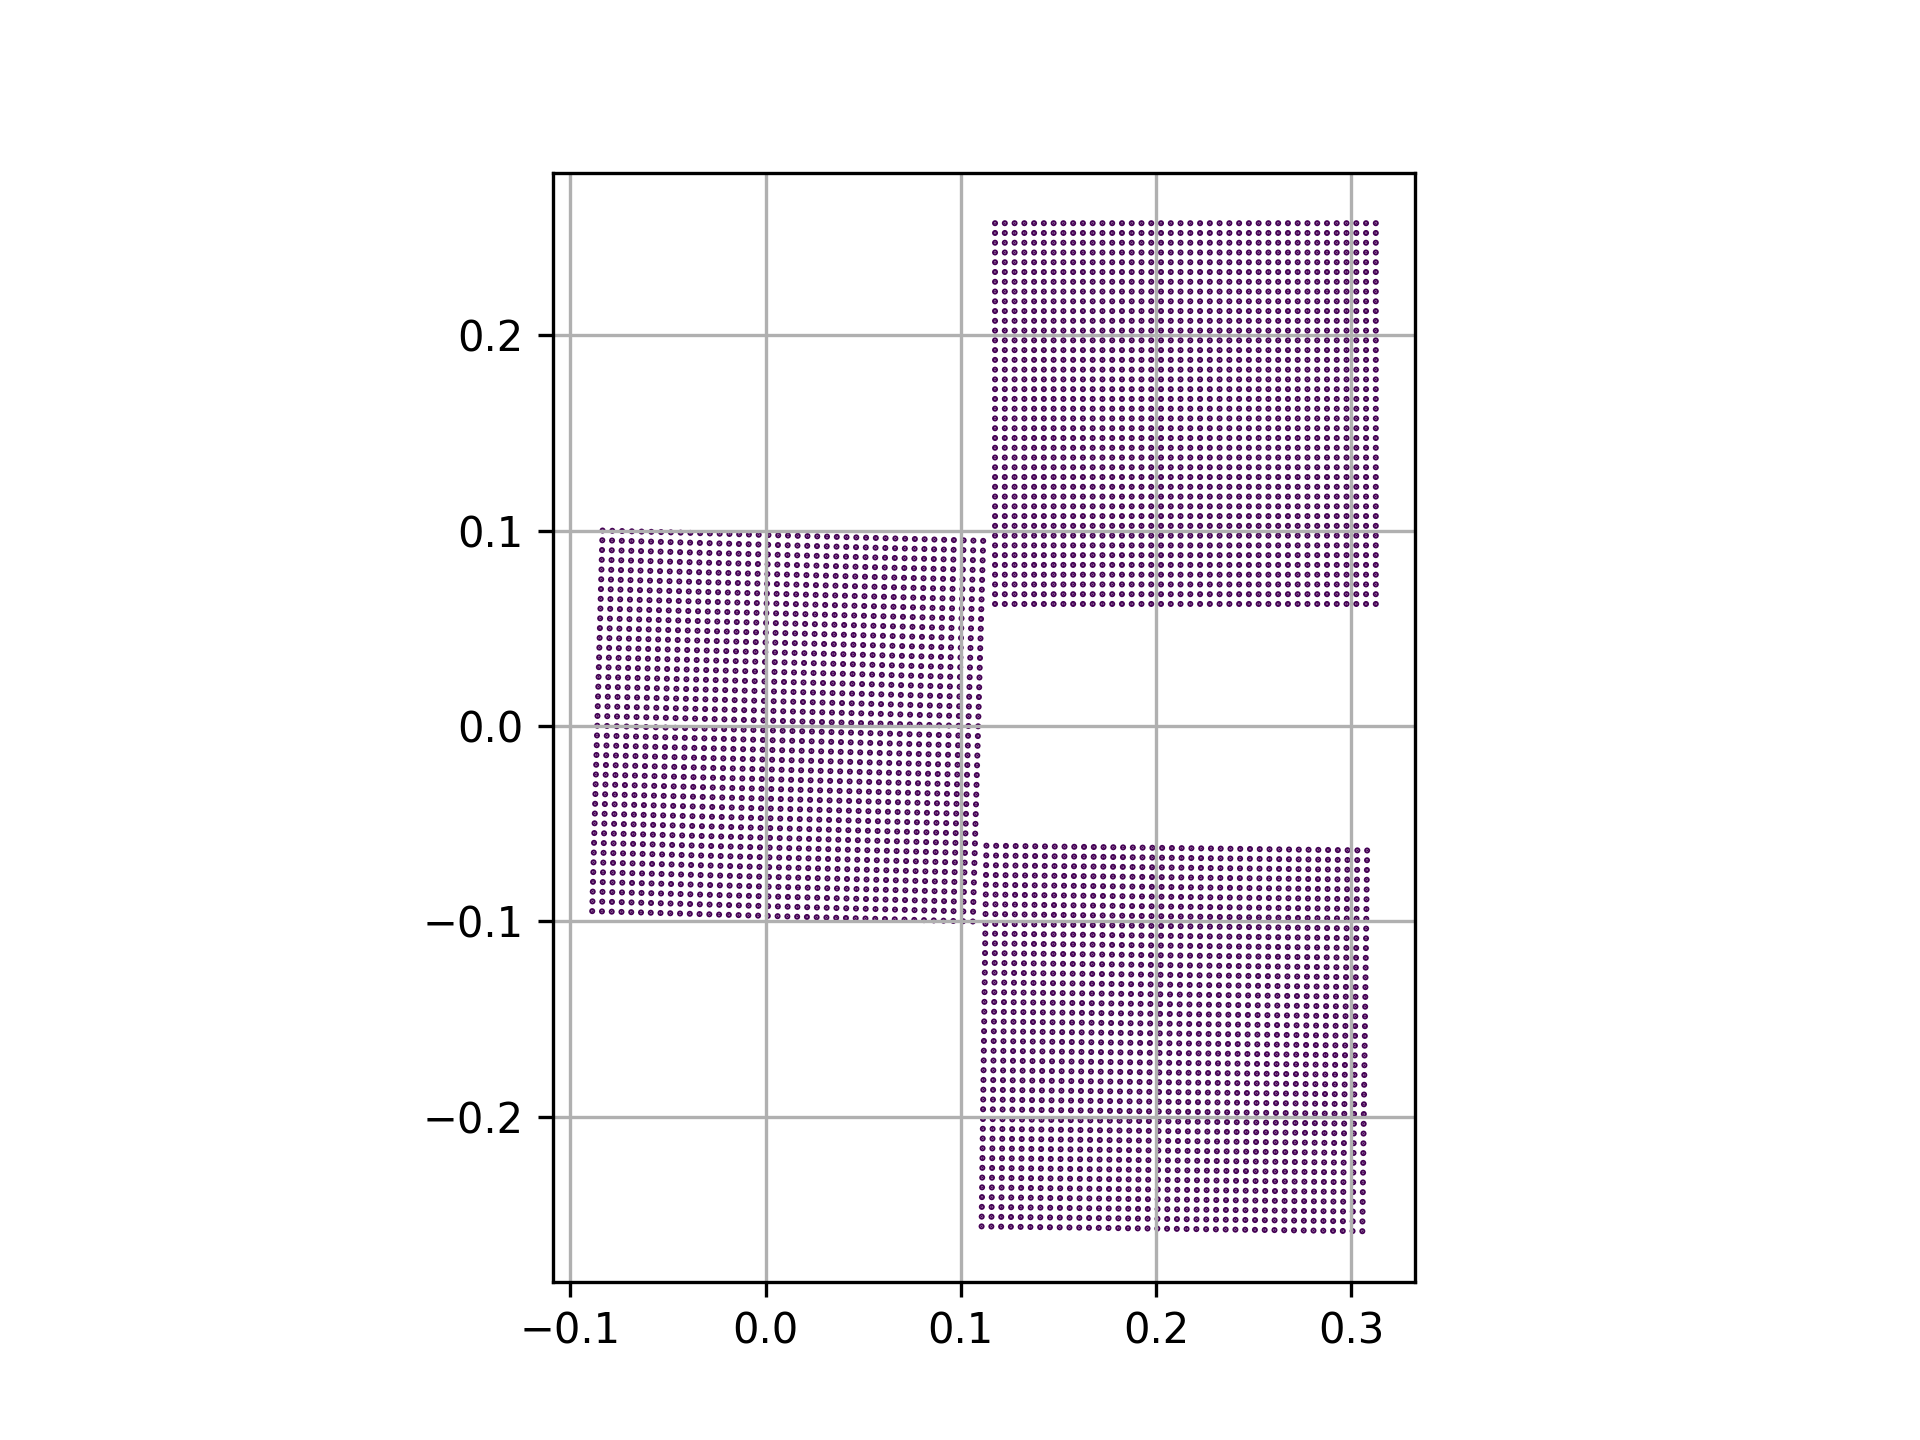
\includegraphics[width=1.0\textwidth]{figures/rfc/figures/amaro_2019_collision_between_three_rigid_cubes/Mohseni_Vyas/time1}
%   \end{subfigure}

%   \begin{subfigure}{0.48\textwidth}
%     \centering
%     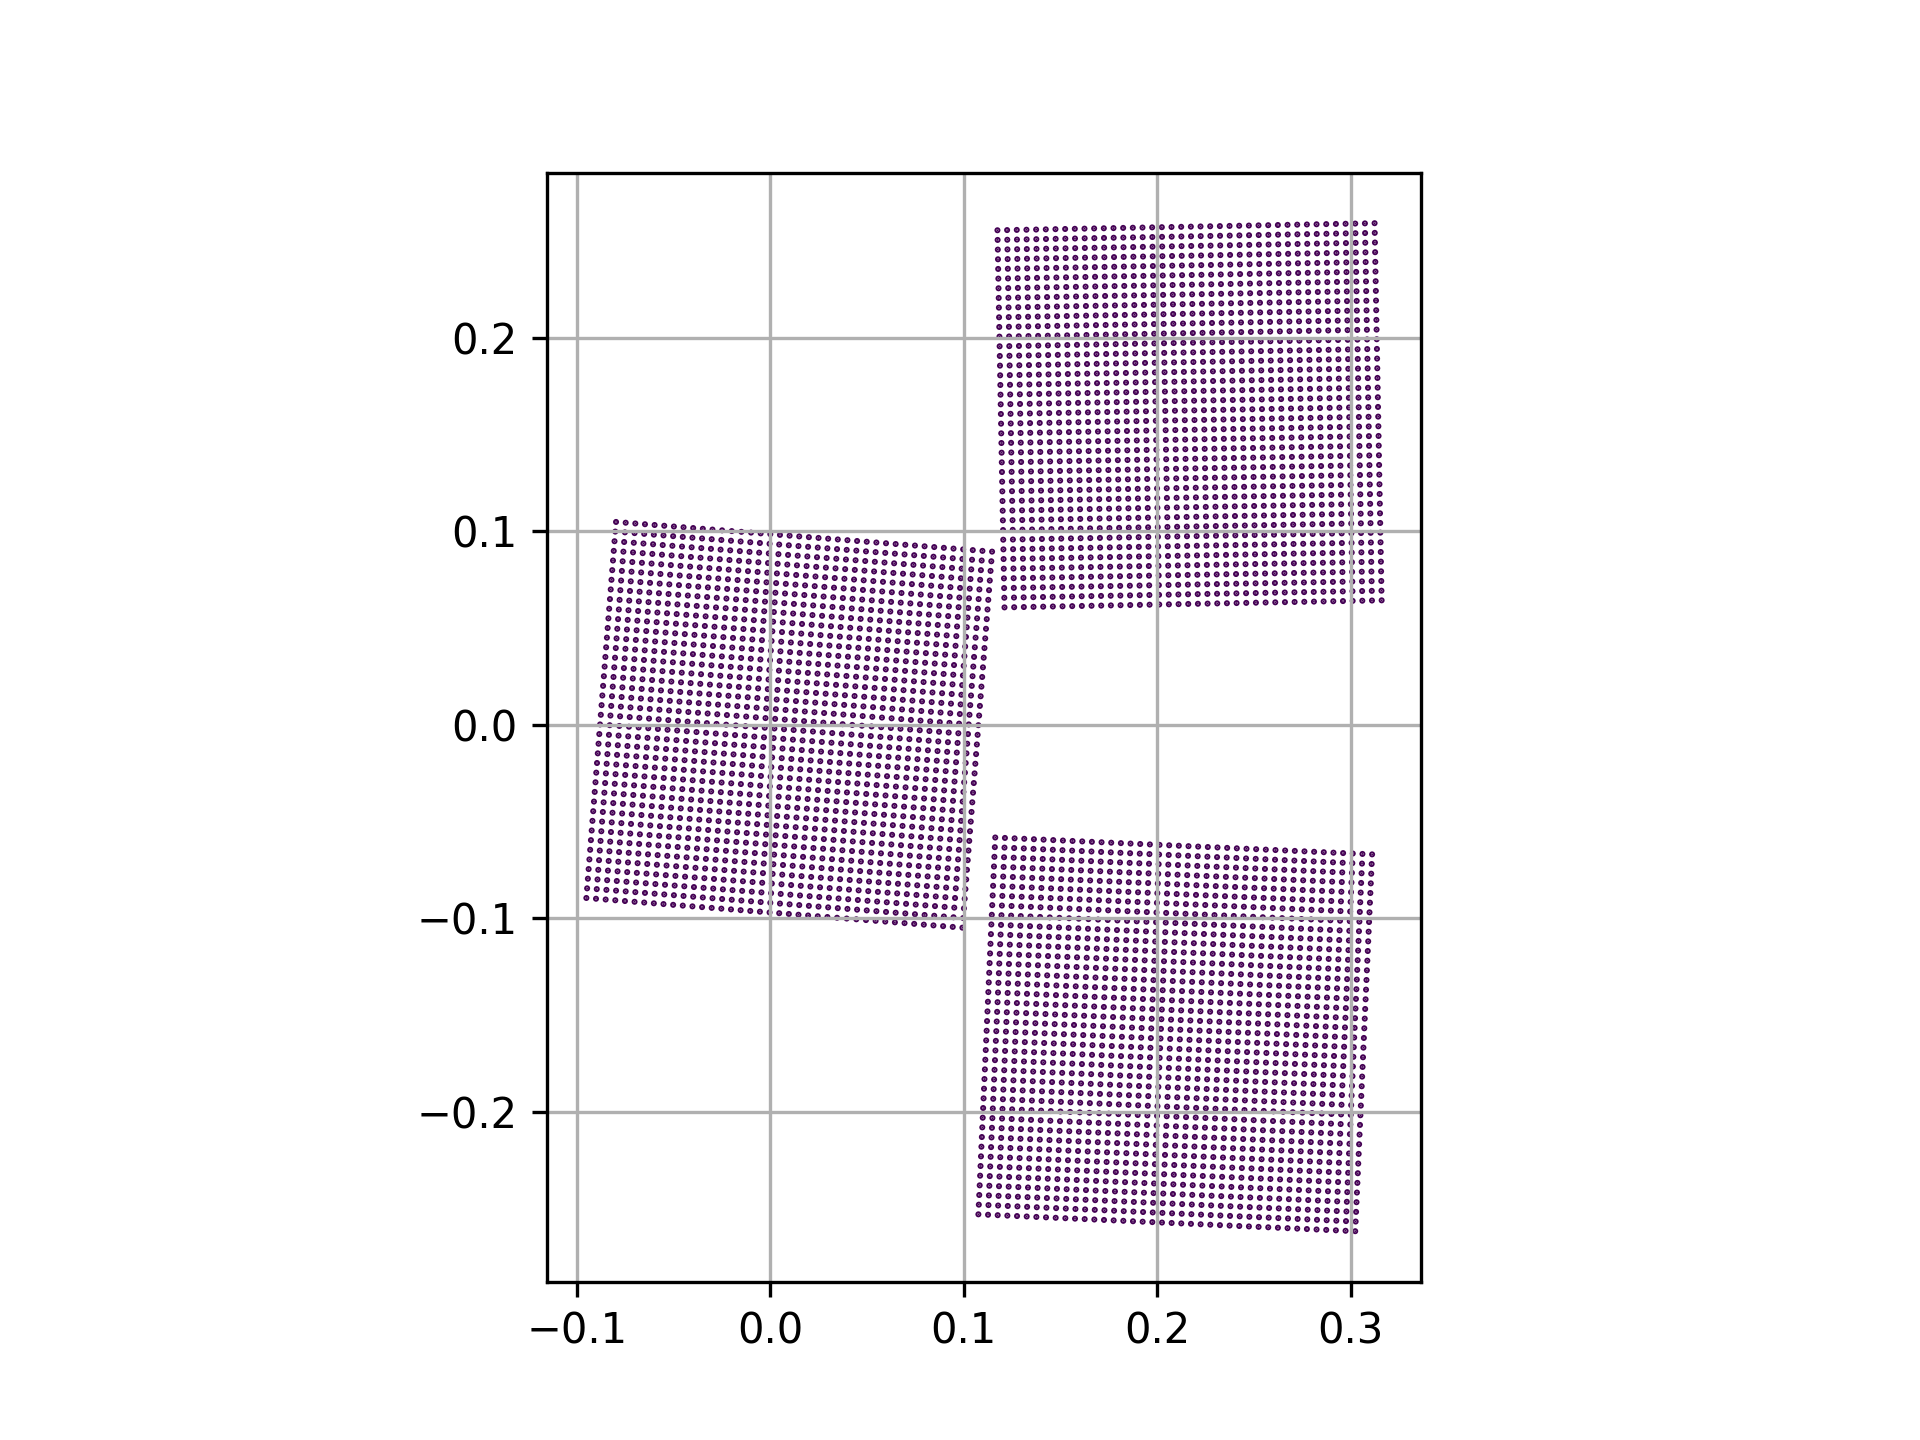
\includegraphics[width=1.0\textwidth]{figures/rfc/figures/amaro_2019_collision_between_three_rigid_cubes/Mohseni_Vyas/time2}
%   \end{subfigure}
%   %
%   \begin{subfigure}{0.48\textwidth}
%     \centering
%     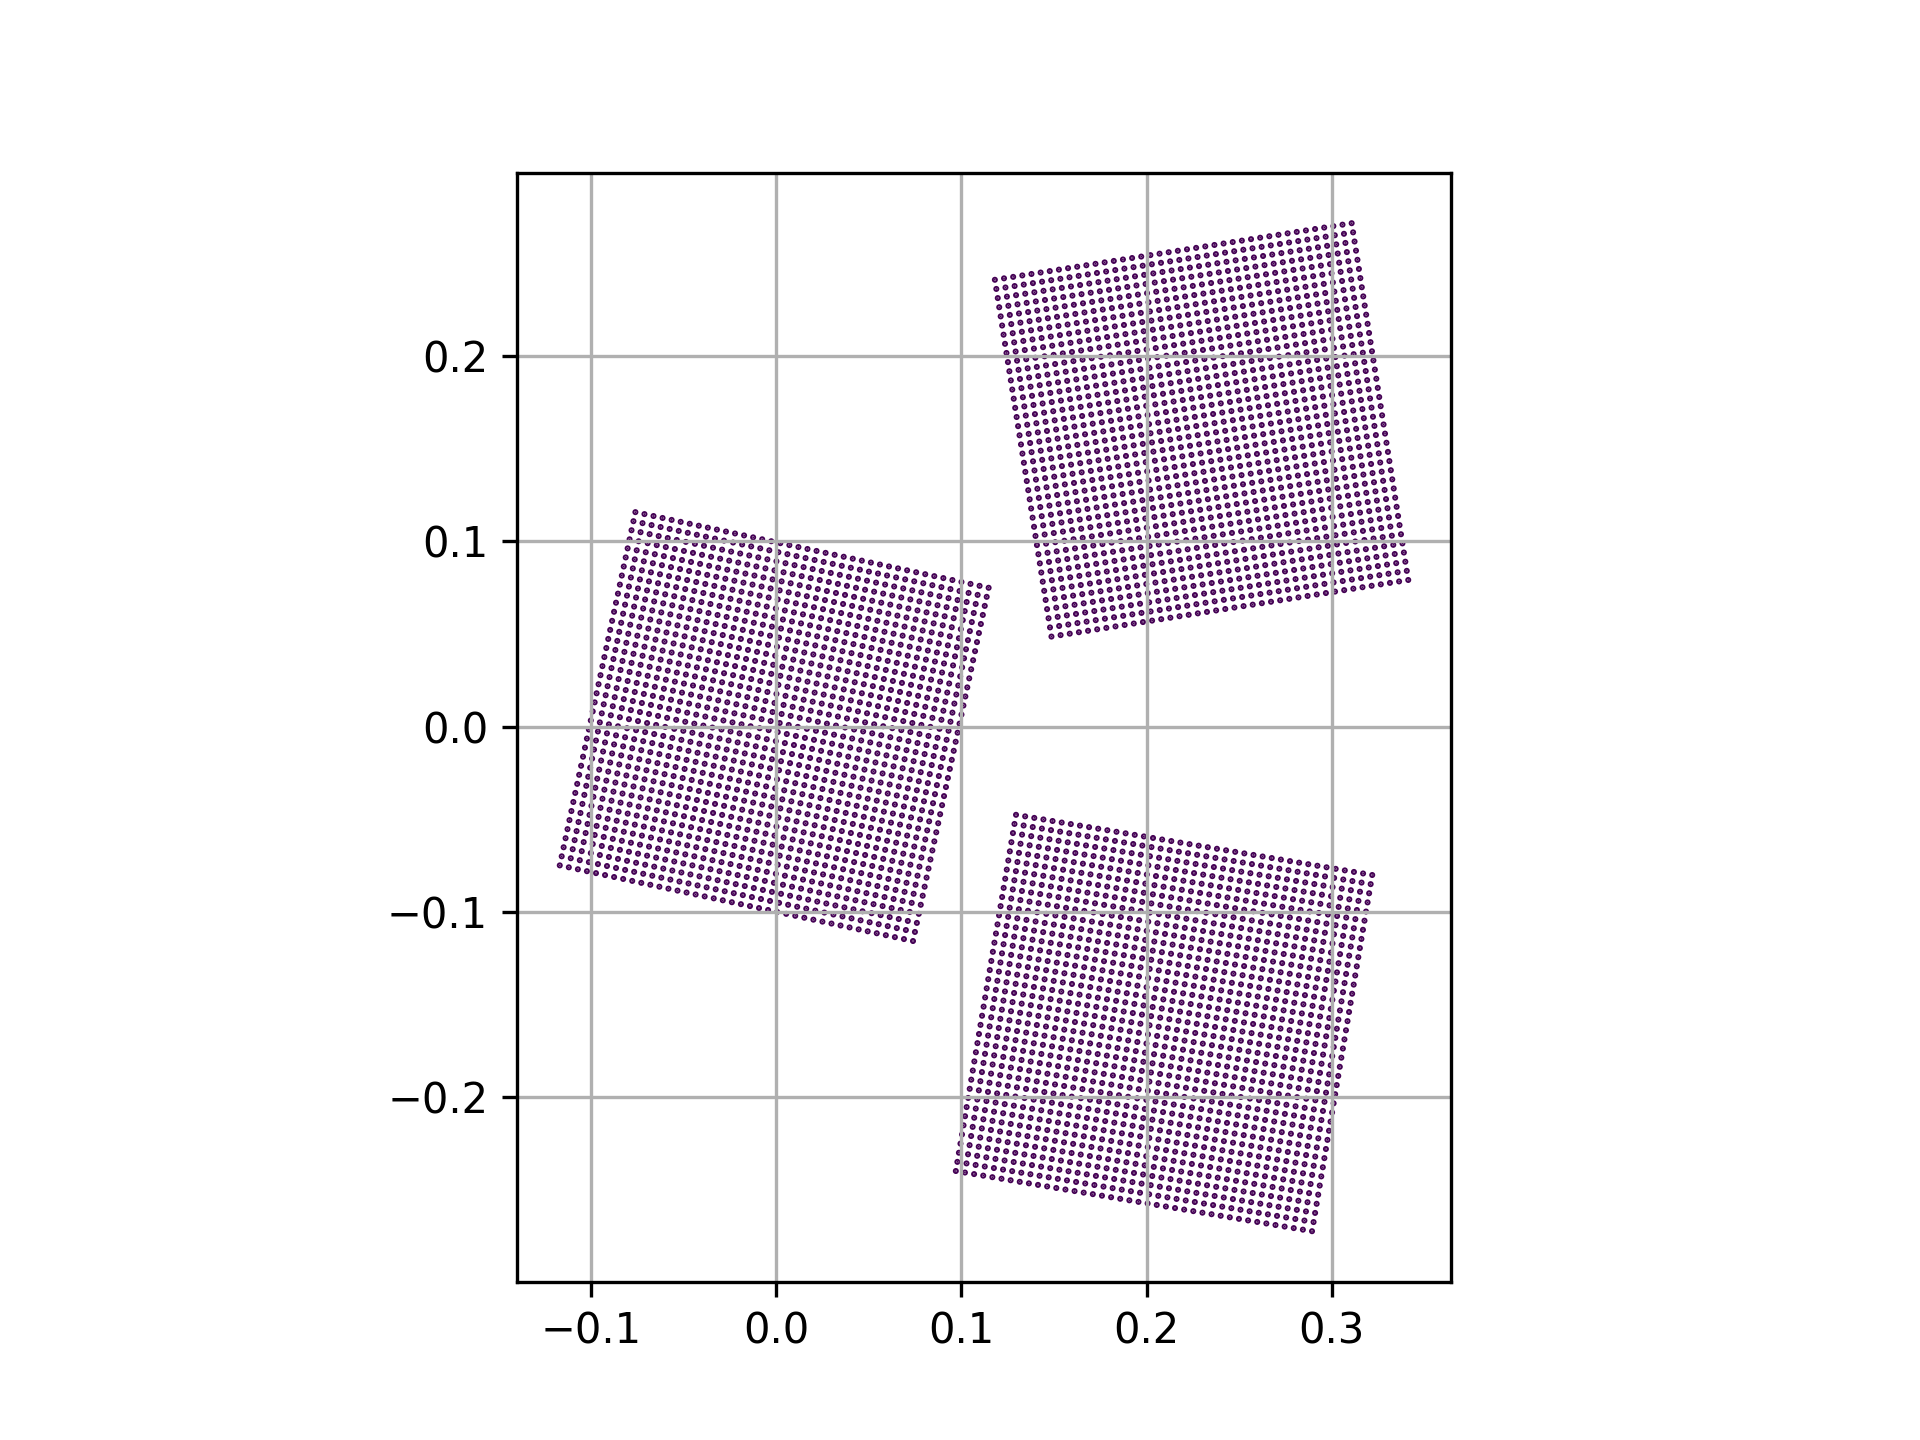
\includegraphics[width=1.0\textwidth]{figures/rfc/figures/amaro_2019_collision_between_three_rigid_cubes/Mohseni_Vyas/time3}
%   \end{subfigure}
% \caption{A dummy figure (To be fixed)}
% \label{fig:snapshots-three-cubes-colliding}
% \end{figure}
% %


\FloatBarrier%
\subsection{Stack of cylinders}
\label{sec:stack-of-cylinders}

This test case is used to validate the current solid-solid contact force model
with the help of a experimental problem. A stack of cylinders initially at rest
are allowed to settle under gravity inside a tank. This experiment is conducted
by \citep{zhang_simulation_2009}, and a numerical analysis is carried out by the
same with DEM. The material and numerical parameters are listed in
\Cref{tab:stack-of-cylinders}.
\begin{table}[!ht]
  \centering
  \begin{tabular}[!ht]{ll}
    \toprule
    Quantity & Values\\
    \midrule
    $L$, length of the tank & $0.26$ m \\
    Diameter of the cylinder & $0.01$ m \\
    Friction coefficient & $0.45$ \\
    $\rho_b$, density of the cylinder & 2700 kg/m\textsuperscript{3} \\
    Spacing, $dx$ & $0.001$m\\
    Normal stiffness, $K_r$ & $10^{7}$ N/m\textsuperscript{1}\\
    Tangential stiffness, $K_t$ & $10^{5}$ N/m\textsuperscript{1}\\
    % Damping coefficient, $K_t$ & $10^{5}$ N/m\textsuperscript{1}\\
    Smoothing length factor, $h/\Delta x$ & 1.0\\
    \bottomrule
  \end{tabular}
  \caption{Numerical and material parameters used in the simulation of collapse
    of stack of cylinders in a tank.}%
  \label{tab:stack-of-cylinders}
\end{table}

\Cref{fig:snapshots-stack-of-cylinders} presents a set of snapshots
corresponding to the simulation of a stack of cylinders collapsing under gravity
using developed solver in comparison with the corresponding experimental photos
by \citep{zhang_simulation_2009}. From the presented
\cref{fig:snapshots-stack-of-cylinders}, the reproduced cylinders' positions
appear to be consistent with those observed in the experiment. From
\cref{fig:snapshots-stack-of-cylinders}, the current solver has presented proper
level of stability.
\begin{figure}[!htpb]
  \centering
  \begin{subfigure}{0.48\textwidth}
    \centering
    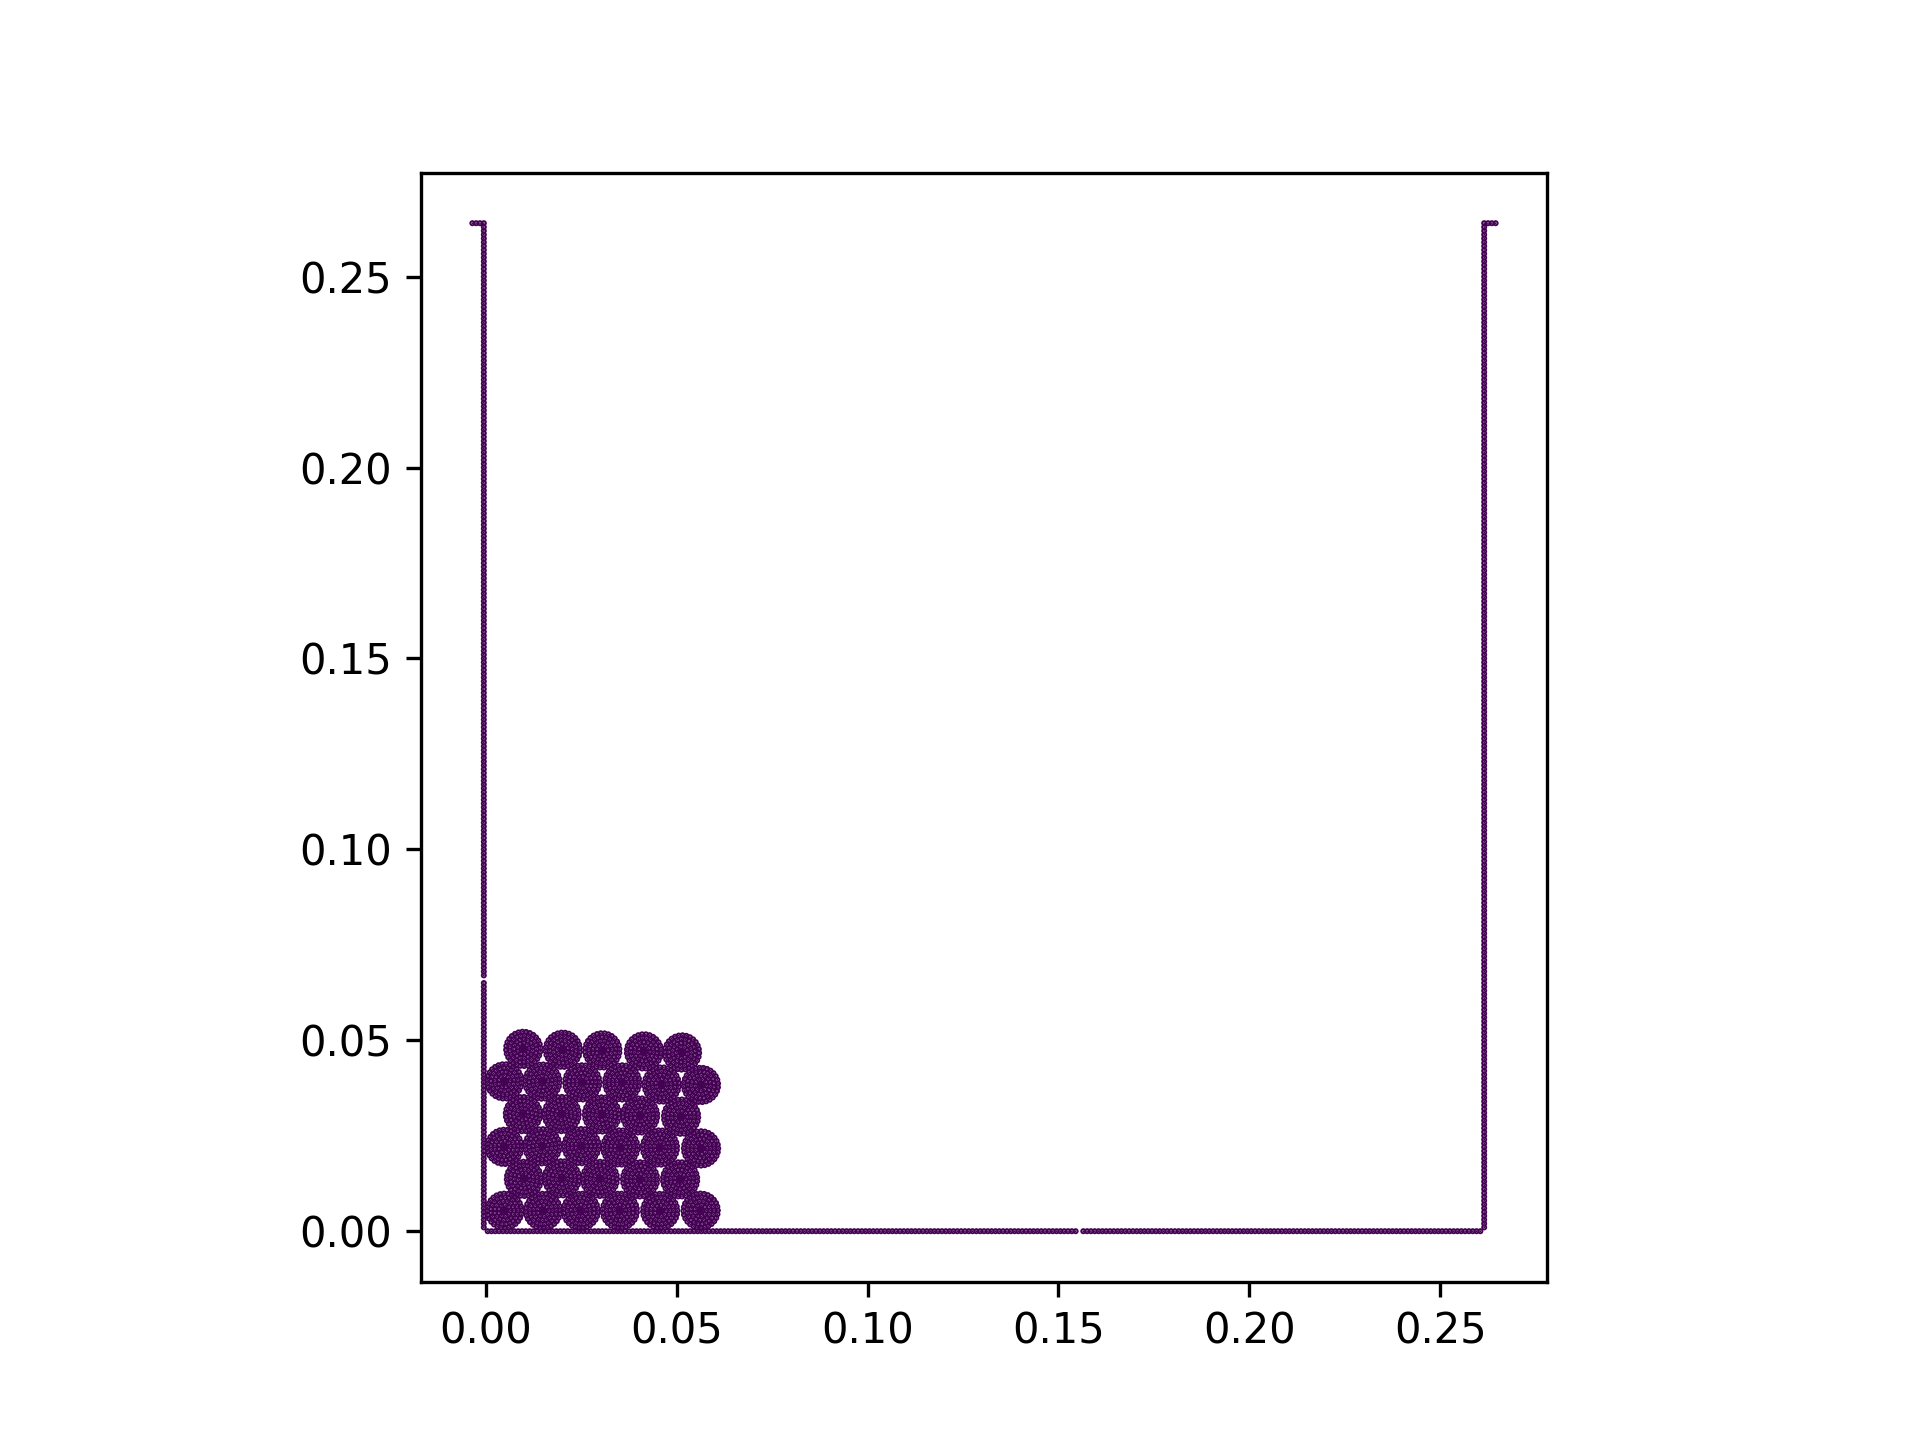
\includegraphics[width=1.0\textwidth]{figures/rfc/figures/stack_of_cylinders_2d/Mohseni_Vyas/time0}
  \end{subfigure}
  %
  \begin{subfigure}{0.48\textwidth}
    \centering
    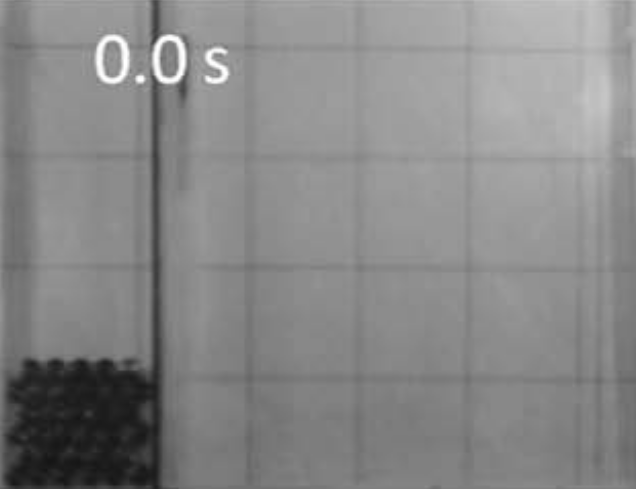
\includegraphics[width=0.75\textwidth]{images/rfc/images/stack_of_cylinders_experimental_images/time0}
  \end{subfigure}

  \begin{subfigure}{0.48\textwidth}
    \centering
    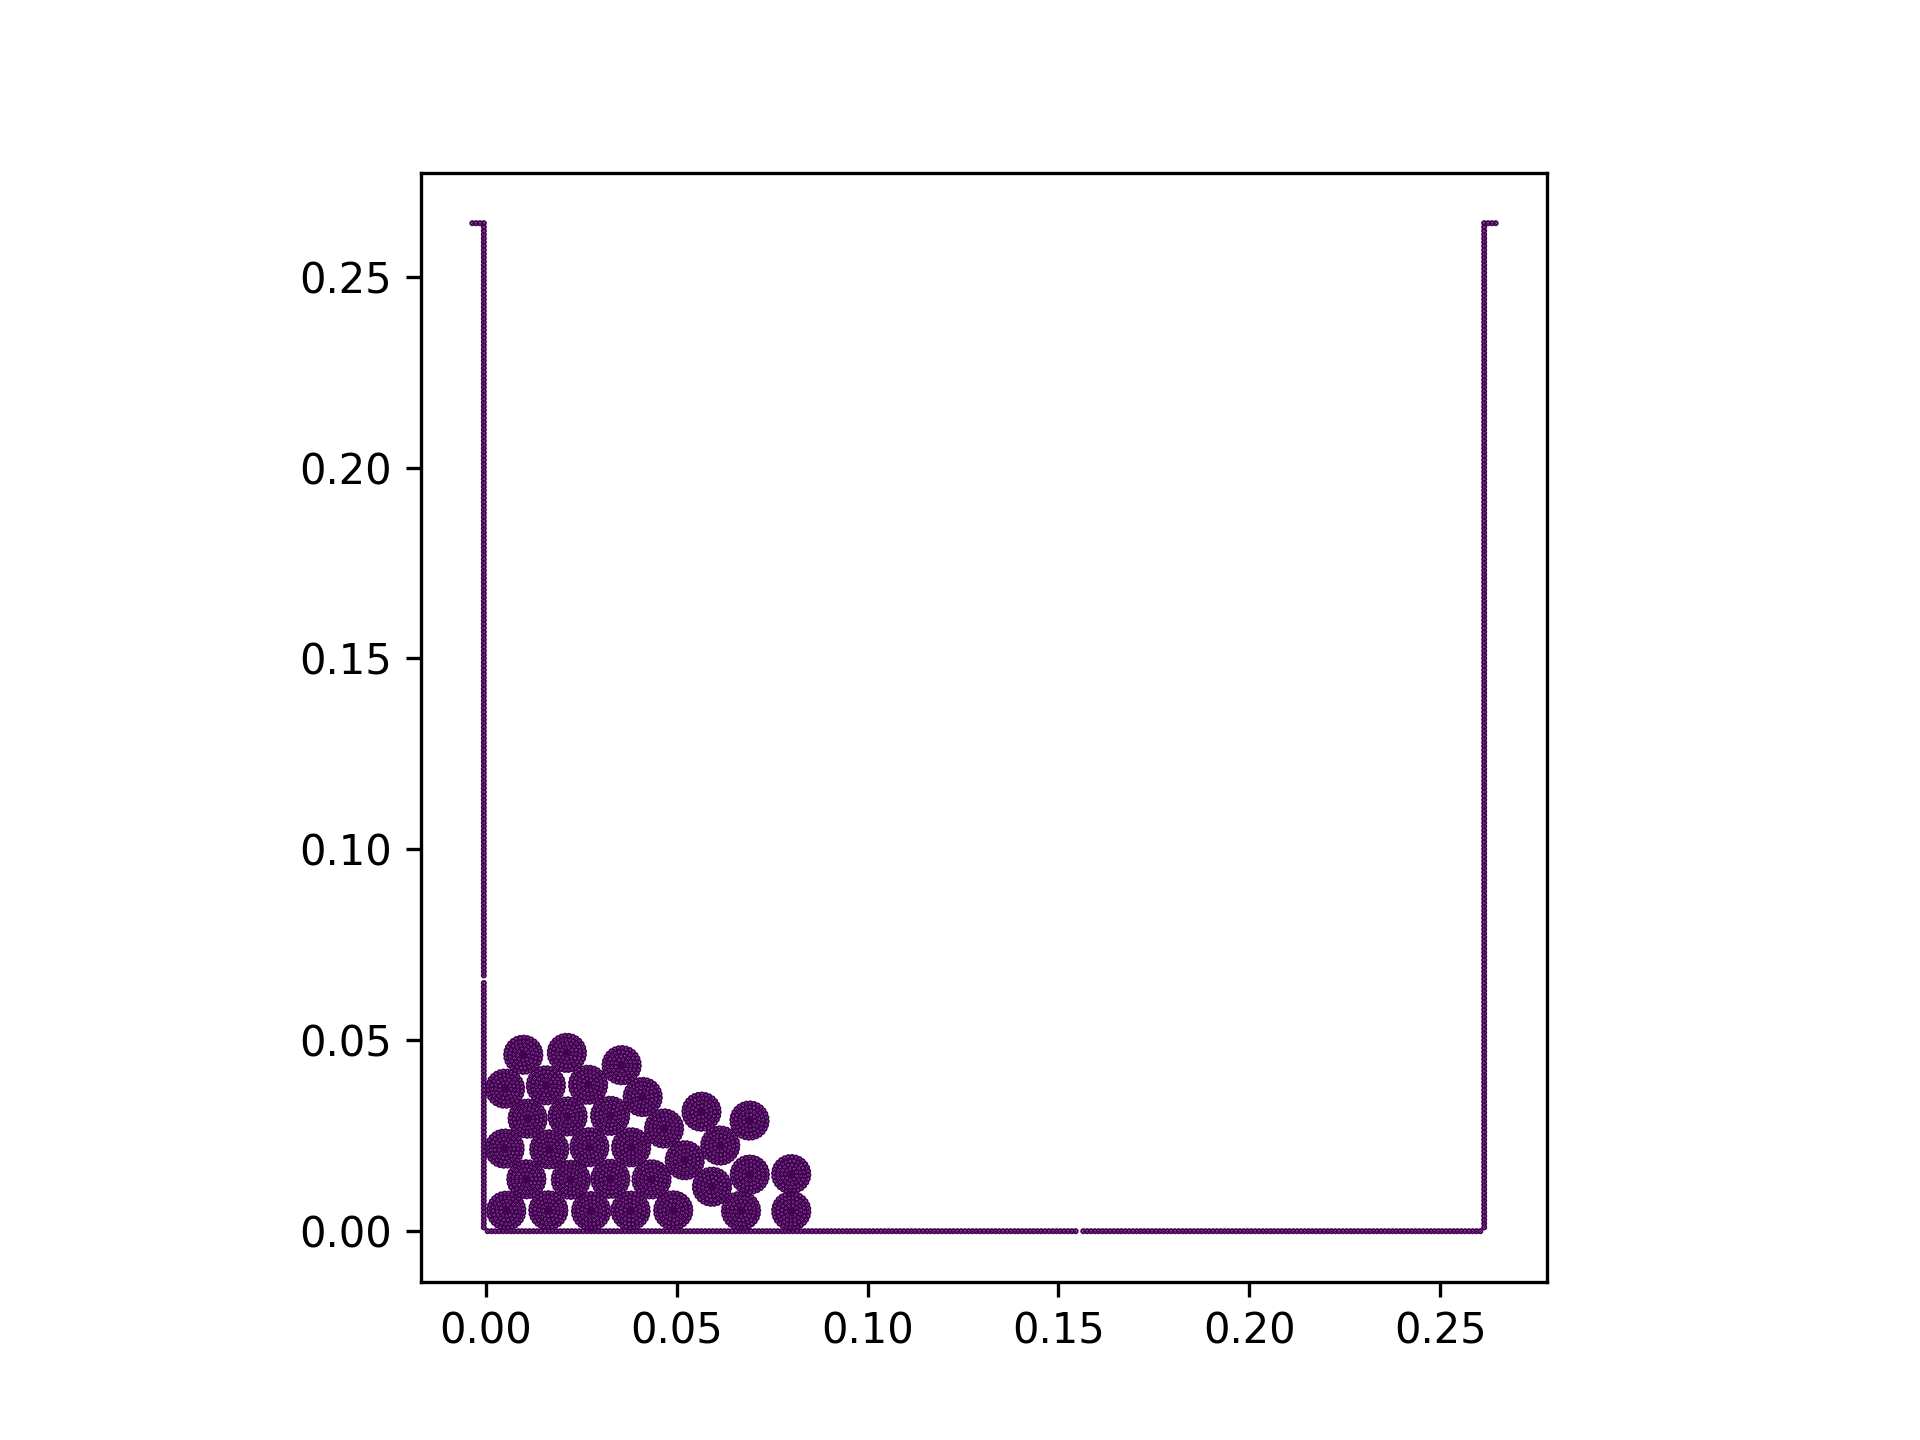
\includegraphics[width=1.0\textwidth]{figures/rfc/figures/stack_of_cylinders_2d/Mohseni_Vyas/time1}
  \end{subfigure}
  %
  \begin{subfigure}{0.48\textwidth}
    \centering
    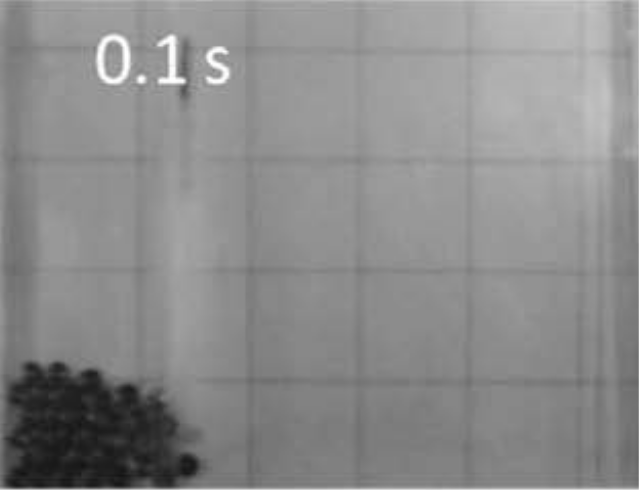
\includegraphics[width=0.75\textwidth]{images/rfc/images/stack_of_cylinders_experimental_images/time1}
  \end{subfigure}

  \begin{subfigure}{0.48\textwidth}
    \centering
    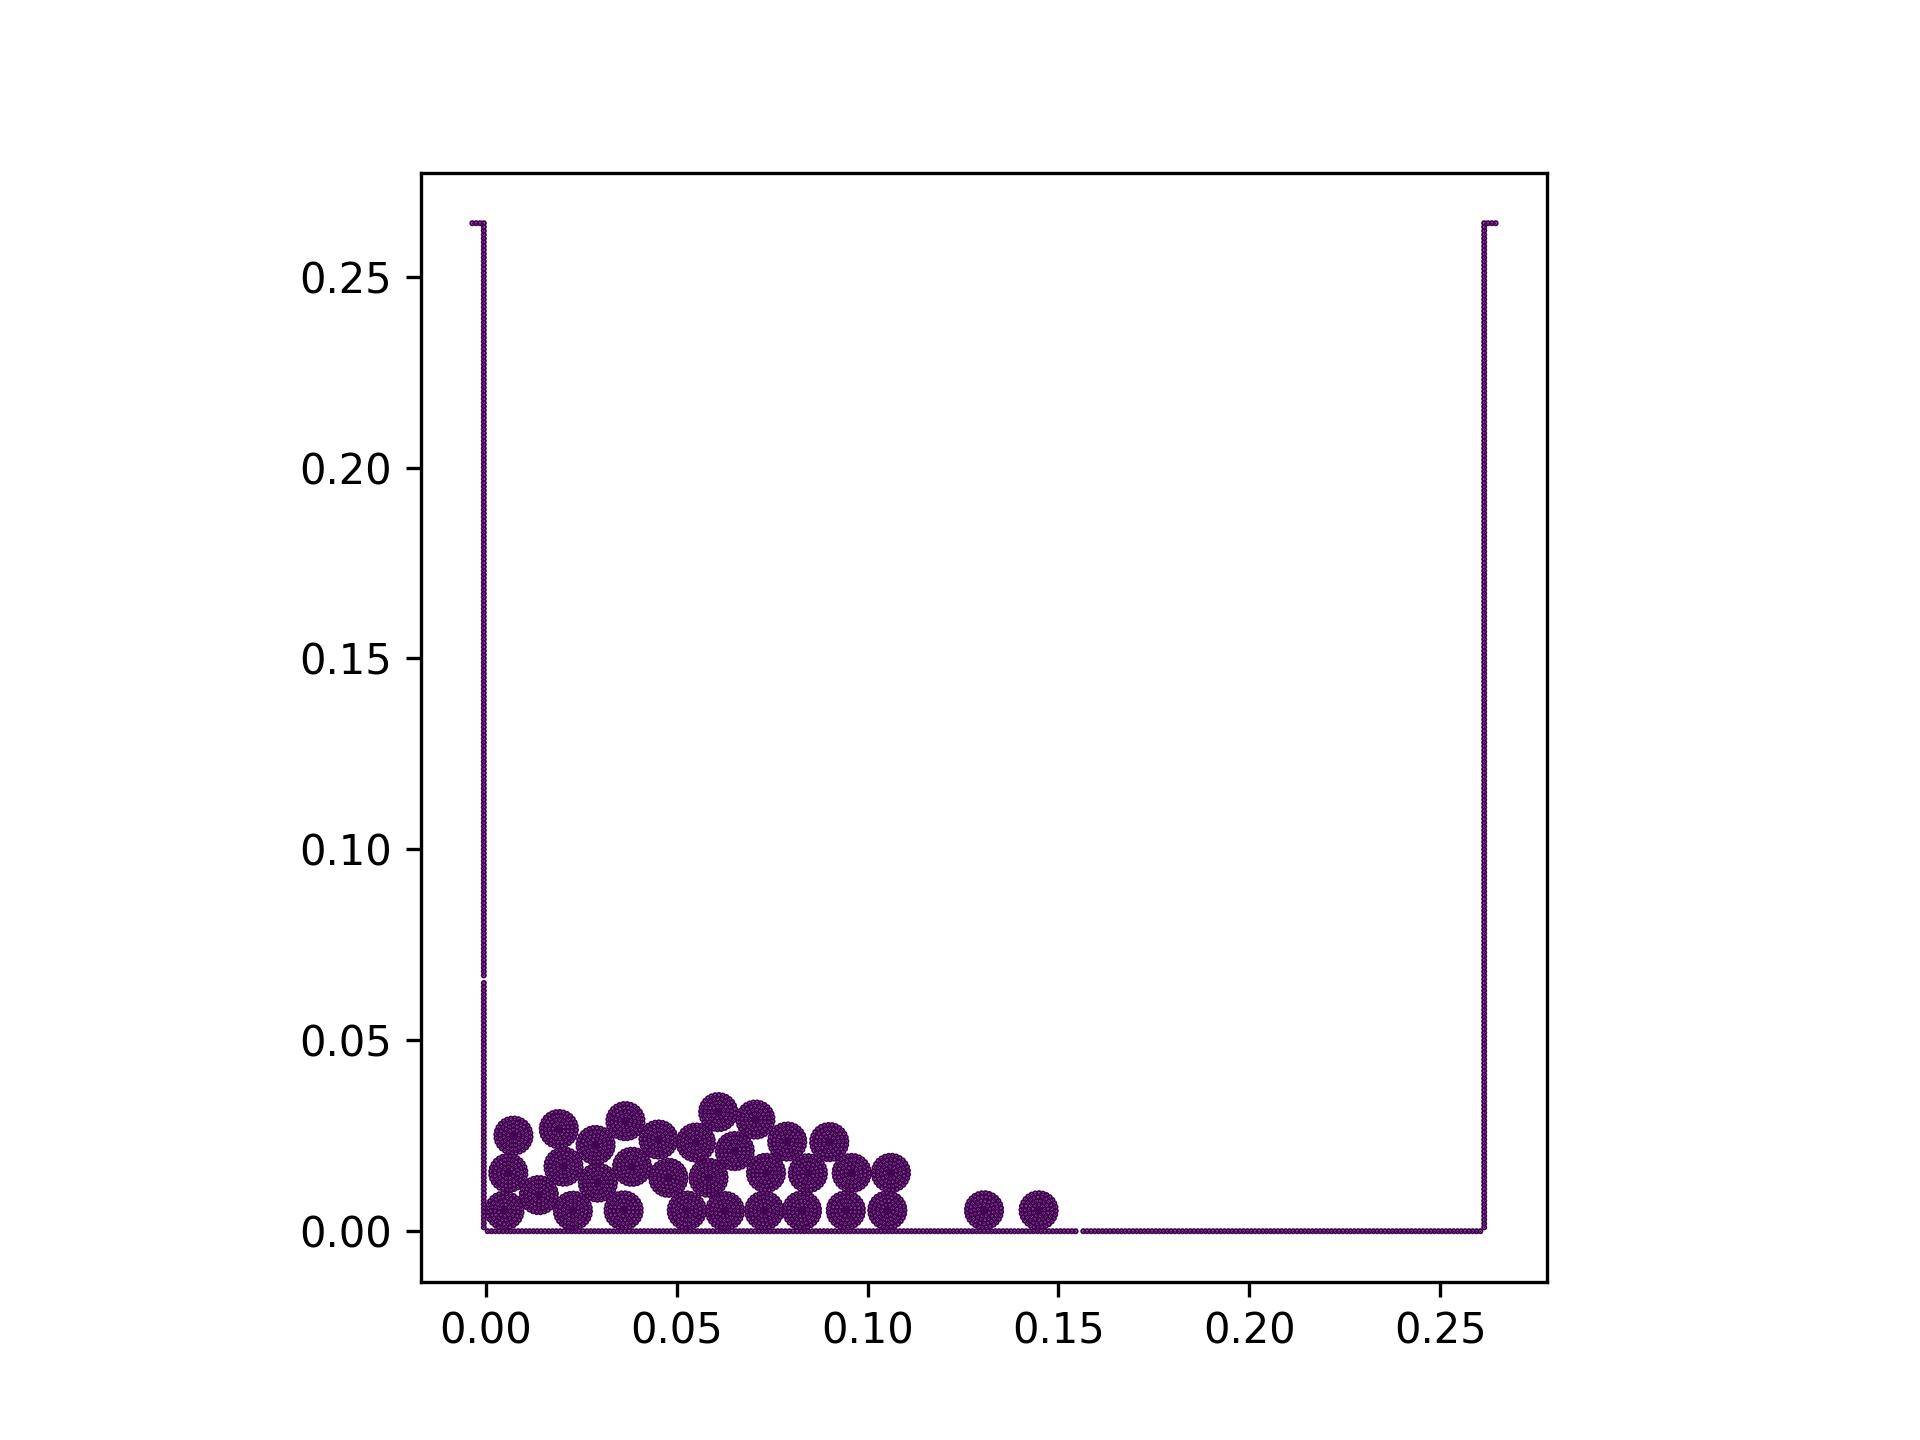
\includegraphics[width=1.0\textwidth]{figures/rfc/figures/stack_of_cylinders_2d/Mohseni_Vyas/time2}
  \end{subfigure}
  %
  \begin{subfigure}{0.48\textwidth}
    \centering
    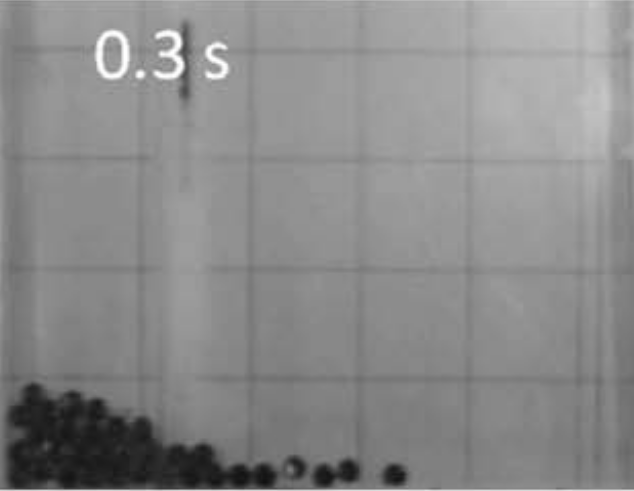
\includegraphics[width=0.75\textwidth]{images/rfc/images/stack_of_cylinders_experimental_images/time2}
  \end{subfigure}

  \begin{subfigure}{0.48\textwidth}
    \centering
    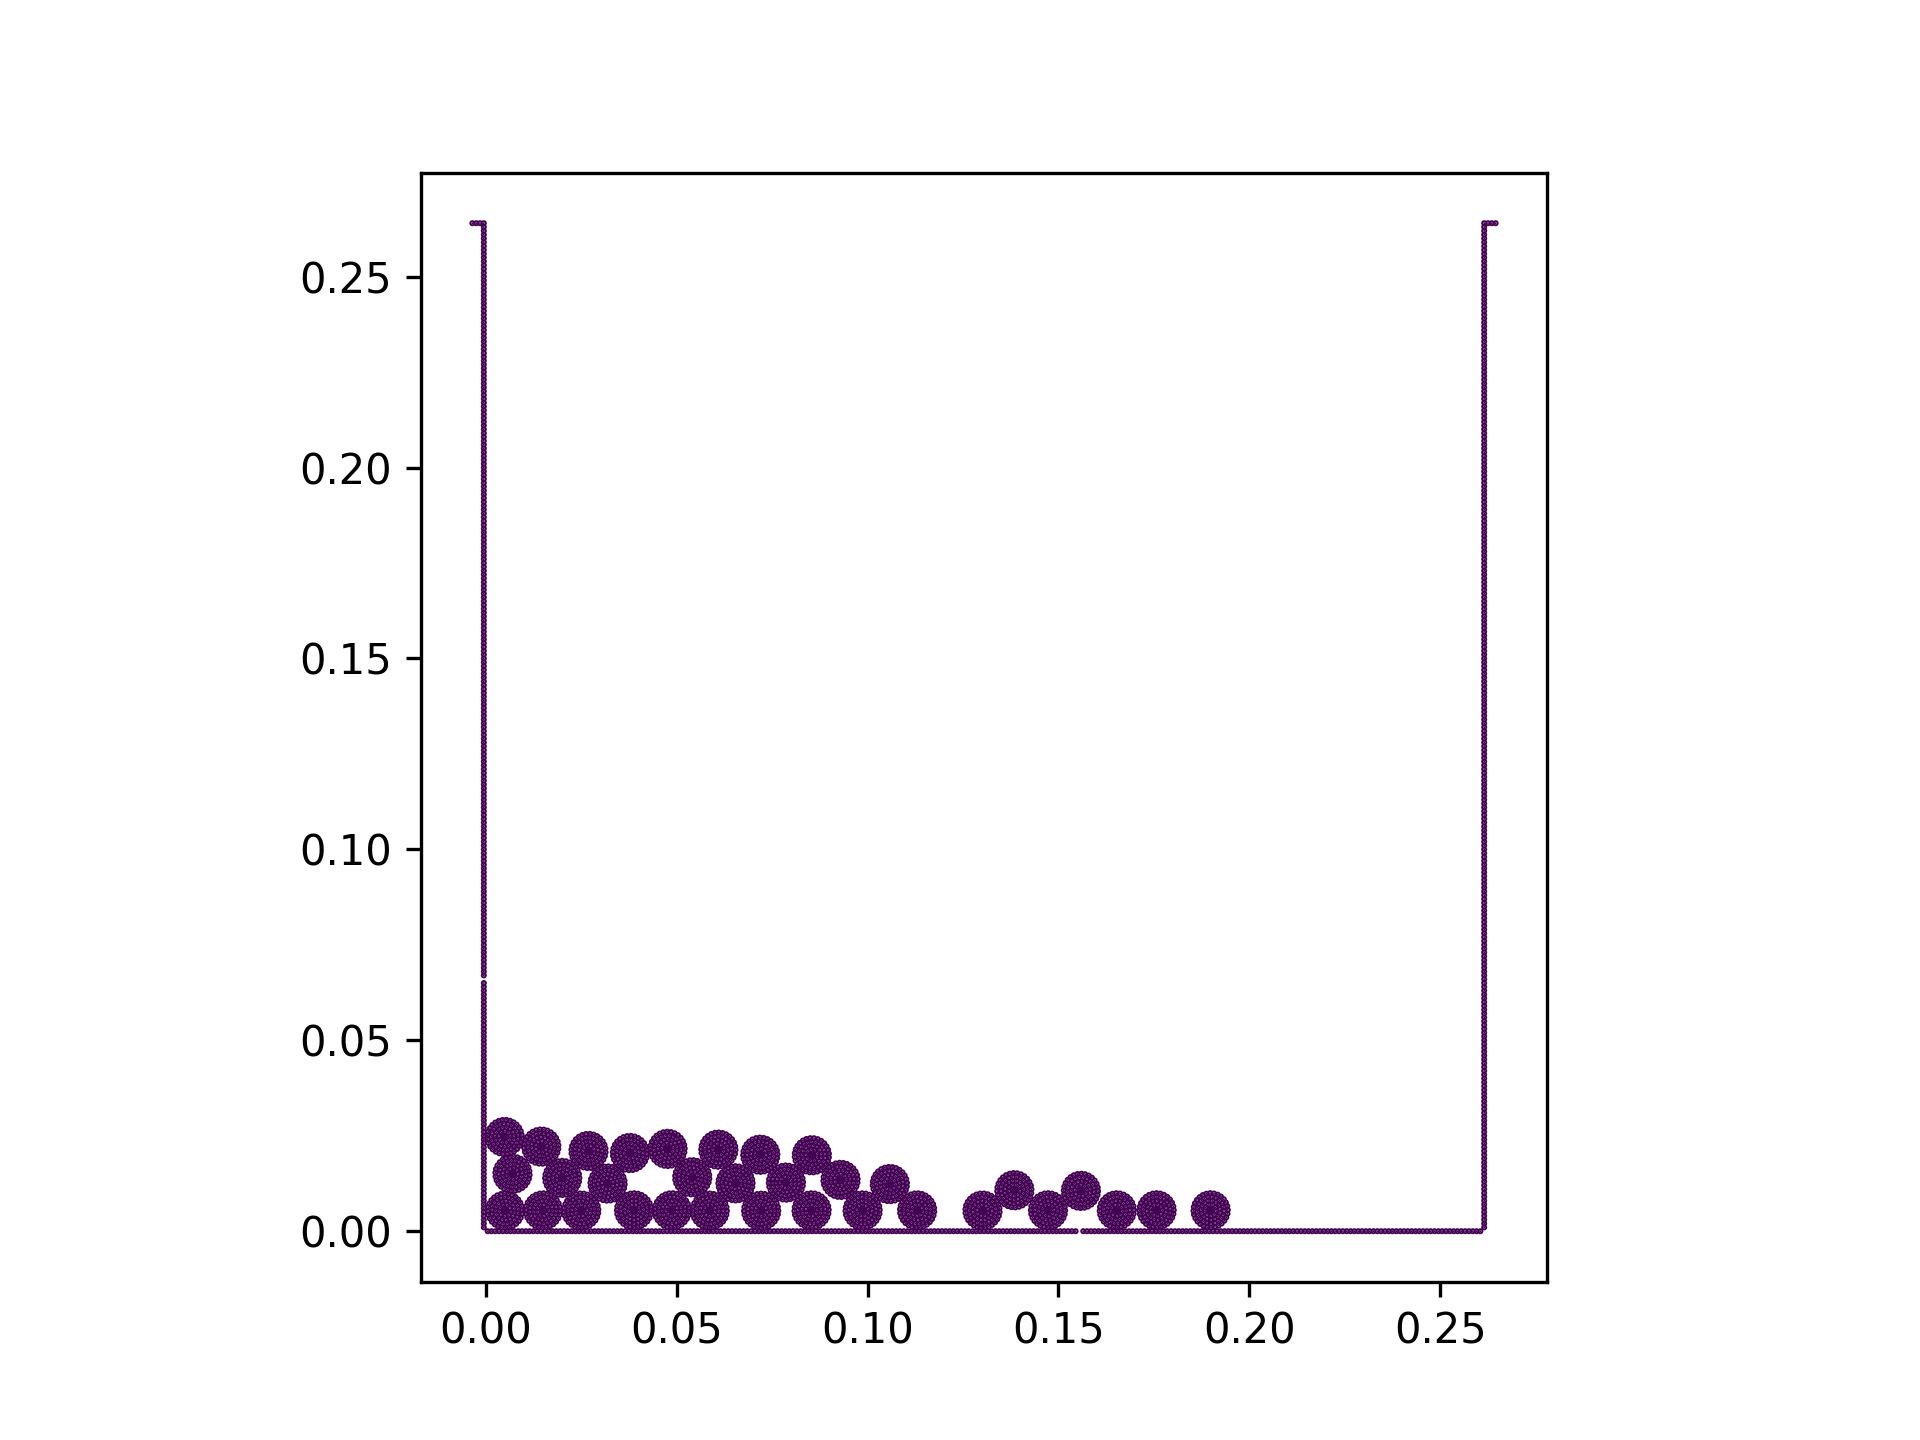
\includegraphics[width=1.0\textwidth]{figures/rfc/figures/stack_of_cylinders_2d/Mohseni_Vyas/time3}
  \end{subfigure}
  %
  \begin{subfigure}{0.48\textwidth}
    \centering
    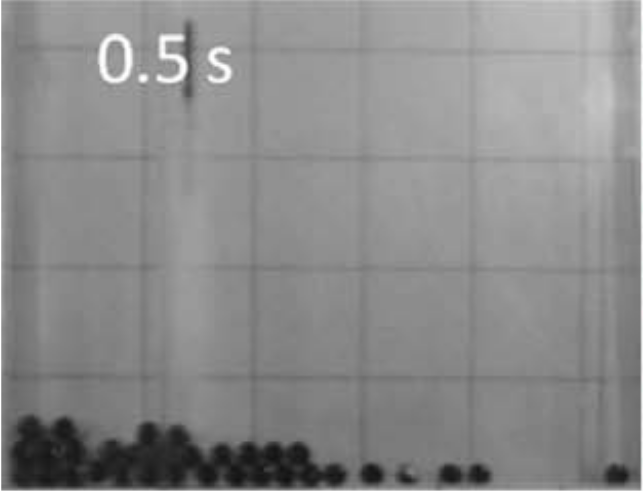
\includegraphics[width=0.75\textwidth]{images/rfc/images/stack_of_cylinders_experimental_images/time3}
  \end{subfigure}
  \caption{Snapshot of the collapsing cylinders at different time stamps
    simulated with the current solver, compared against the experimental
    pictures \citep{zhang_simulation_2009}.}
\label{fig:snapshots-stack-of-cylinders}
\end{figure}
%


\Cref{fig:x-com-stack-of-cylinders,fig:y-com-stack-of-cylinders} presents the
time histories of the x and y components of the center of mass of the cylinders
respectively as well as those from the experimental result of
\citep{zhang_simulation_2009}. From the presented figure, we can see that the
effective center of mass of the cylinders is in good agreement with the
experiment.
\begin{figure}[!htpb]
  \centering
  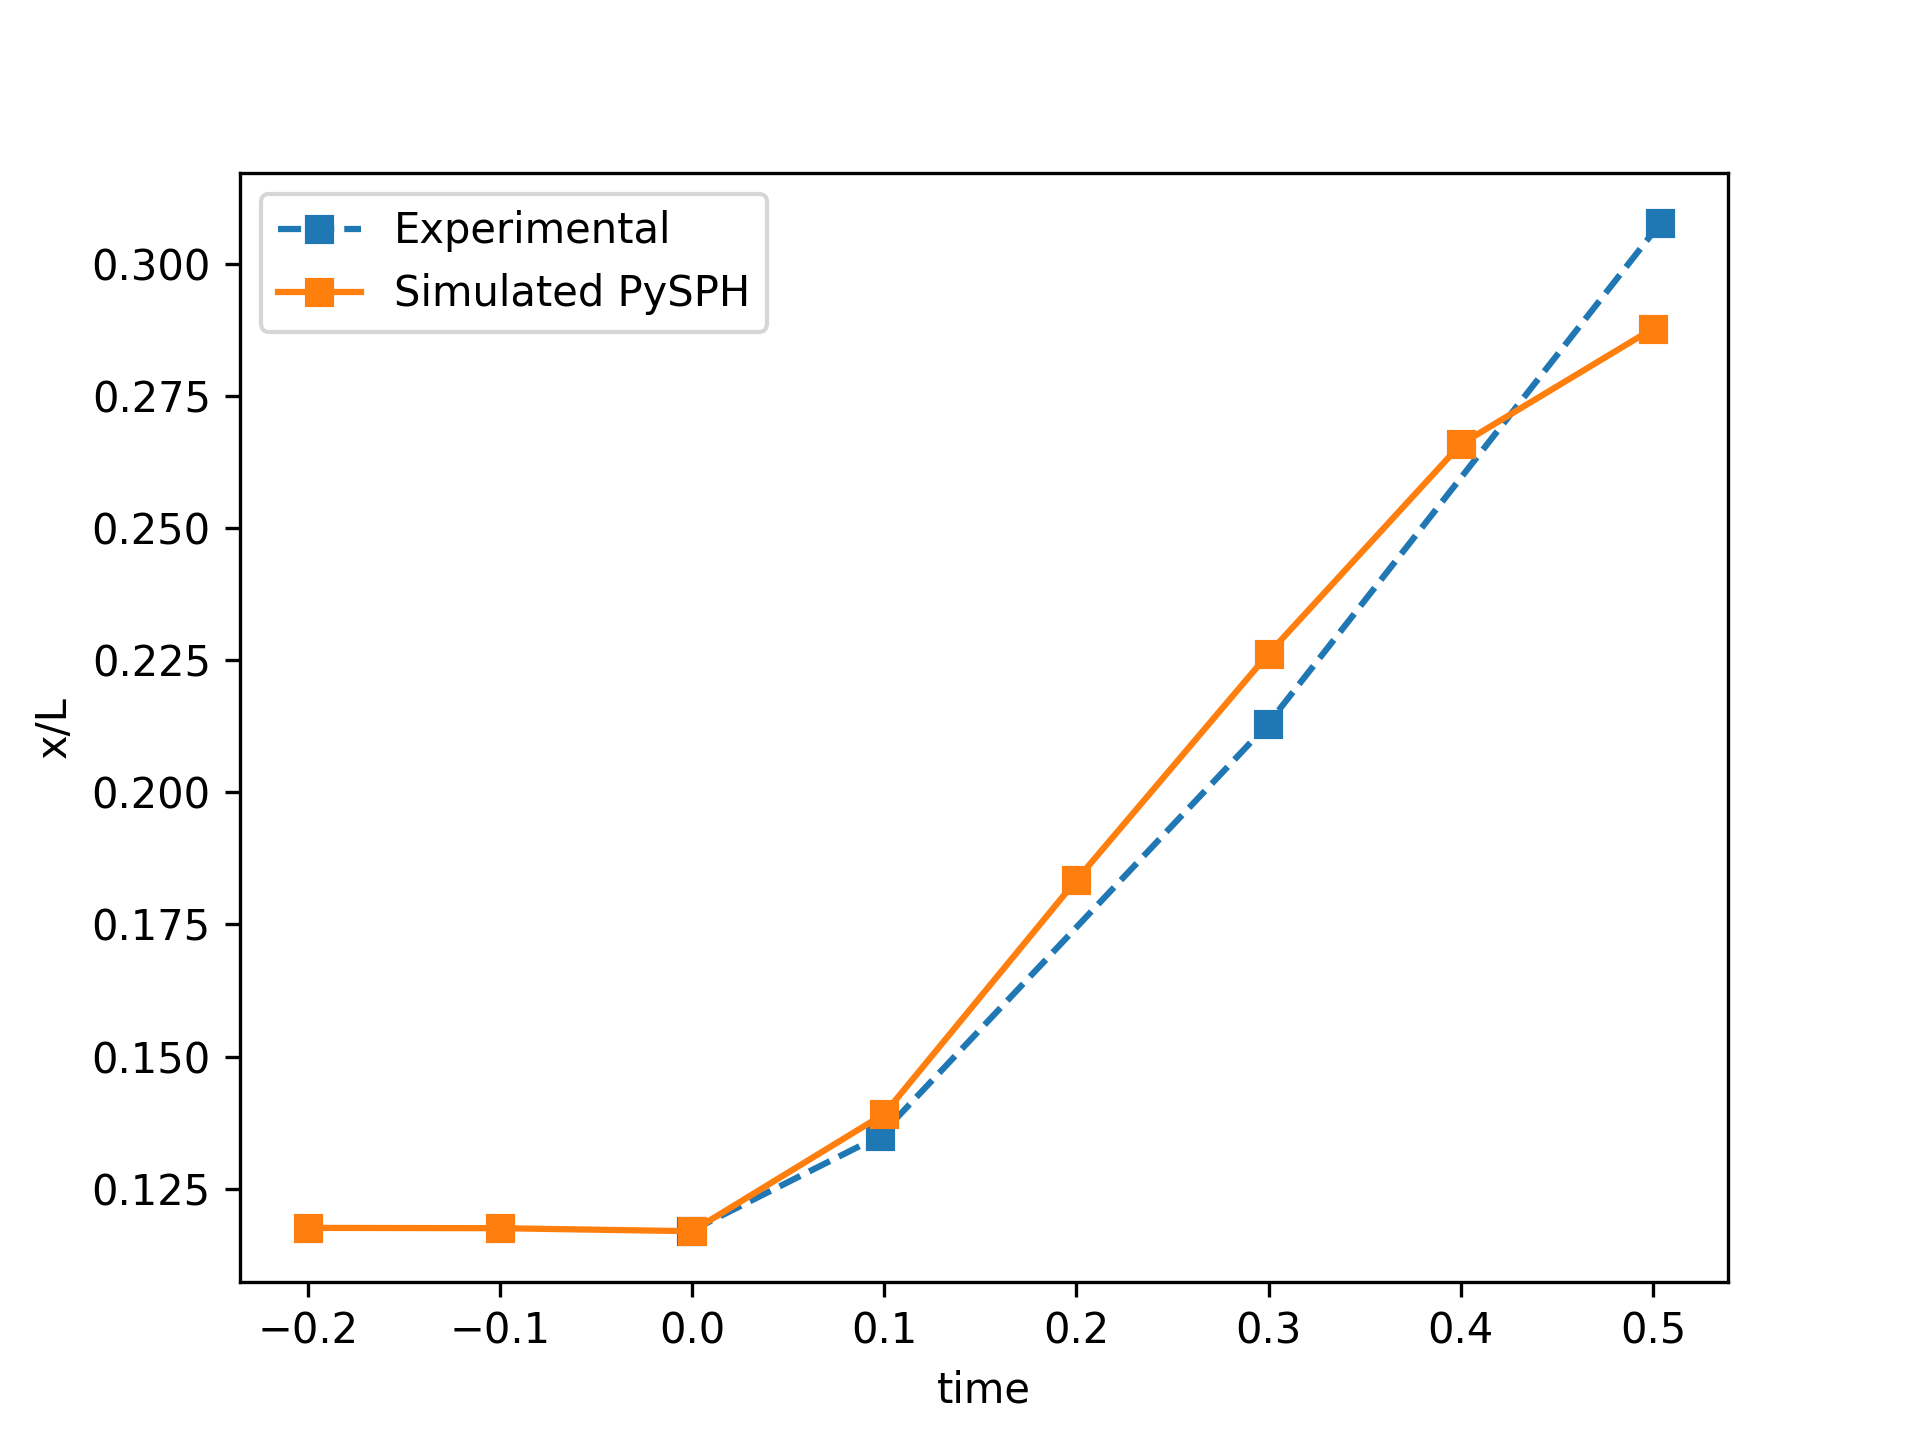
\includegraphics[width=0.4\textwidth]{figures/rfc/figures/stack_of_cylinders_2d/Mohseni_Vyas/xcom}
  \caption{Variation of the x-component of the center of mass of the collapsing
    cylinders computed using the current solver compared against experimental
    results.}
\label{fig:x-com-stack-of-cylinders}
\end{figure}
\begin{figure}[!htpb]
  \centering
  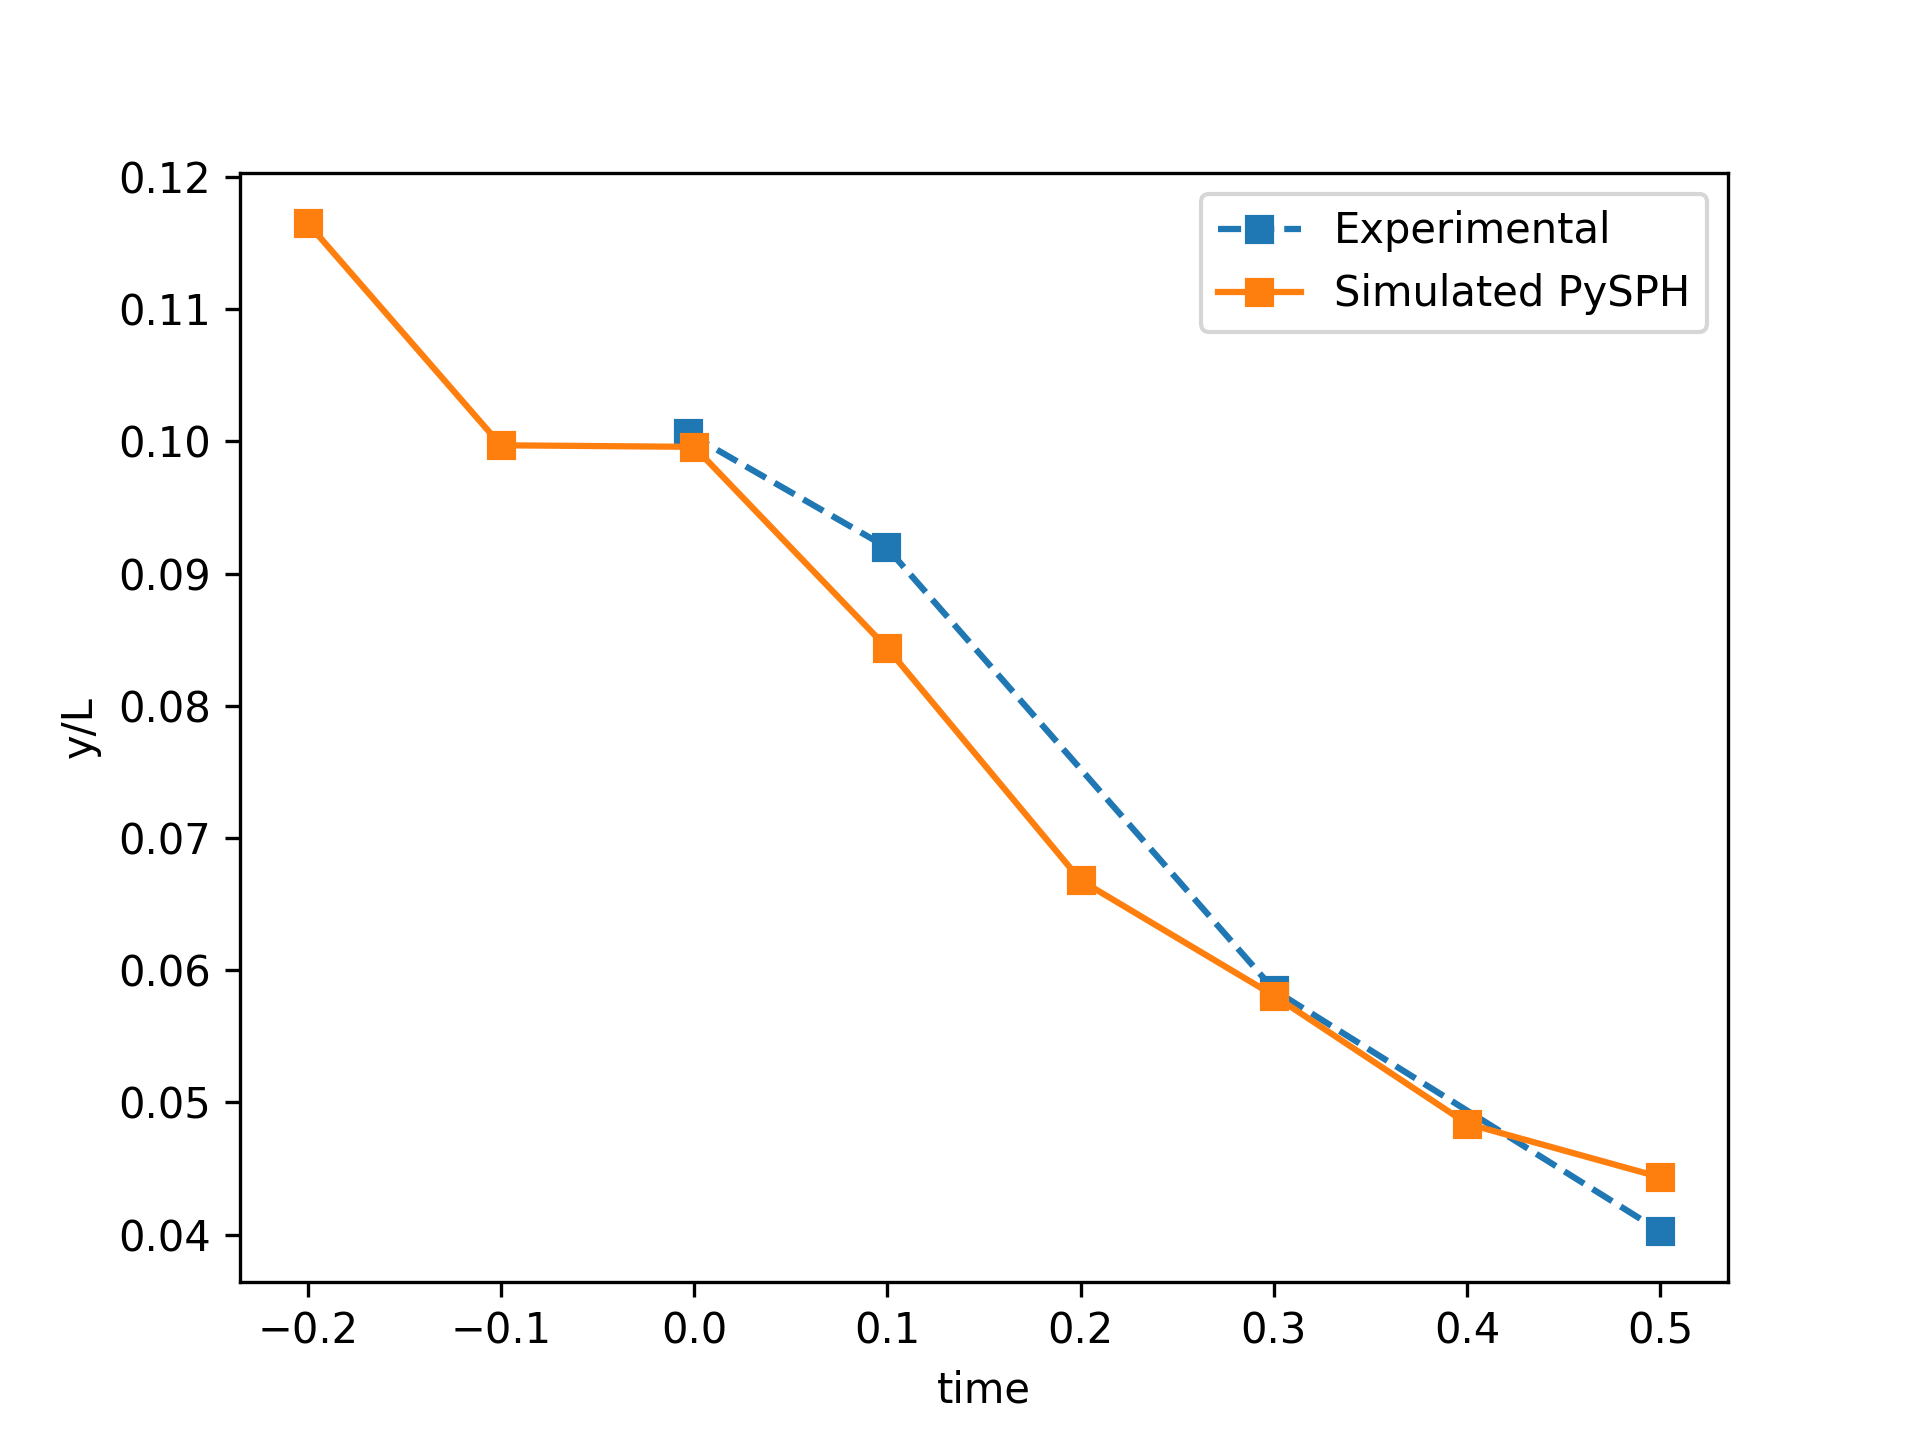
\includegraphics[width=0.4\textwidth]{figures/rfc/figures/stack_of_cylinders_2d/Mohseni_Vyas/ycom}
  \caption{Variation of the y-component of the center of mass of the collapsing
    cylinders computed using the current solver compared against experimental
    results.}
\label{fig:y-com-stack-of-cylinders}
\end{figure}


\FloatBarrier%
\subsection{Falling cube of density 2200 kg/m\textsuperscript{3} in a steady
  hydrostatic tank in water}
\label{sec:falling-solid-in-water}
In this section, the rigid fluid coupling part of the current solver is
evaluated by simulation of a rigid cube falling in an hydrostatic tank
\citep{qiu_3d_2017}. The CTVF-DEM solver is employed to simulate water entry of
a rigid cube, which is studied experimentally by (Wu). The numerical and
material parameters of the current test case are listed in
\cref{tab:rfc:qiu-falling-cube}.
\begin{table}[!ht]
  \centering
  \begin{tabular}[!ht]{ll}
    \toprule
    Quantity & Values\\
    \midrule
    $L$, length of the domain & 1 m \\
    Time of simulation & 2.5 s \\
    $c_s$ & 10 m/s \\
    $\rho_0$, reference density & 1 kg/m\textsuperscript{3} \\
    Reynolds number & 200 \& 1000 \\
    Resolution, $L/\Delta x_{\max} : L/\Delta x_{\min}$ & $[100:200]$ \& $[150:300]$\\
    Smoothing length factor, $h/\Delta x$ & 1.0\\
    \bottomrule
  \end{tabular}
  \caption{Numerical and material parameters used in the simulation of water
    entry of a rigid cube.}%
  \label{tab:rfc:qiu-falling-cube}
\end{table}

A rigid cube of a side length of 30 mm enters the water initially at hydrostatic
state with a velocity of 30 $m/s$ in z-direction.
\Cref{fig:snapshots-falling-solid-in-water} presents a snapshots of the rigid
cube falling in an hydrostatic tank with the current solver as well as WCSPH-DEM
solver as well as the experimental result. From the presented figure
\Cref{fig:snapshots-falling-solid-in-water}, we can see that the pressure
distribution is smooth and the simulation is stable. From
\cref{fig:snapshots-falling-solid-in-water} we can see that the fluid
particle distribution around the body with CTVF scheme is uniform, this
is because of the transport velocity formulation.
\begin{figure}[!htpb]
  \centering
  \begin{subfigure}{0.48\textwidth}
    \centering
    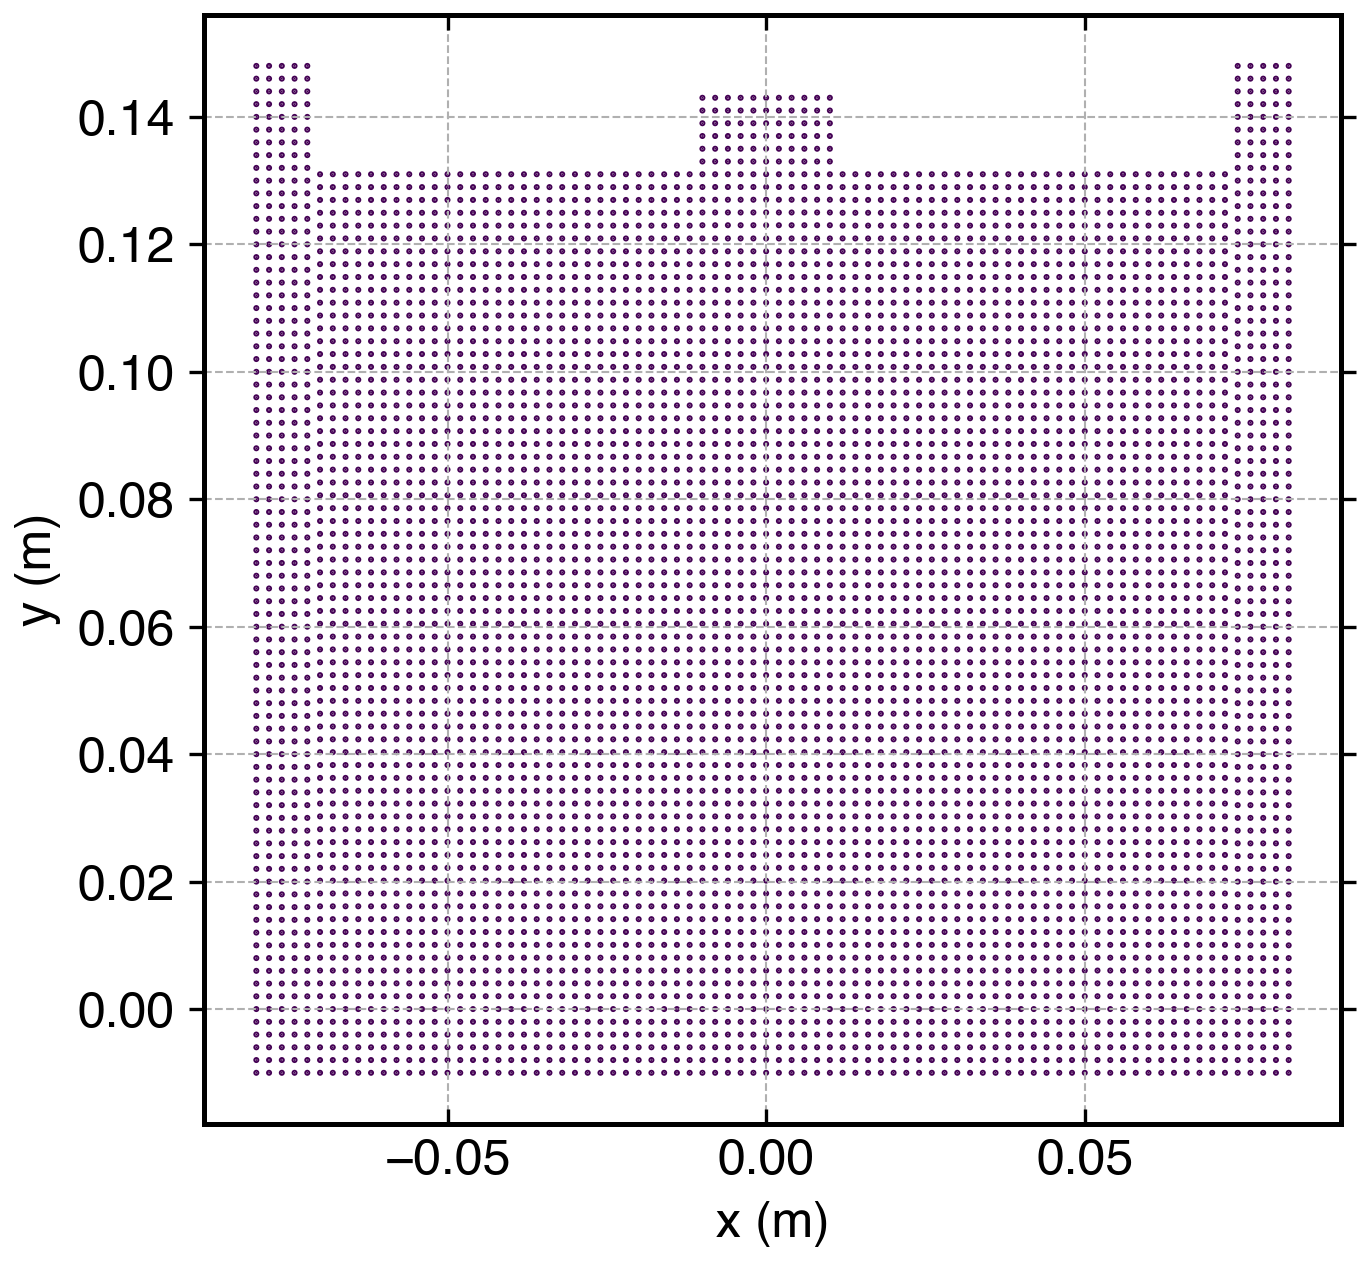
\includegraphics[width=1.0\textwidth]{figures/rfc/figures/qiu_2017_falling_solid_in_water_2d/dx_0_002/time0}
    \subcaption{t = $0$ sec}
  \end{subfigure}
  %
  \begin{subfigure}{0.48\textwidth}
    \centering
    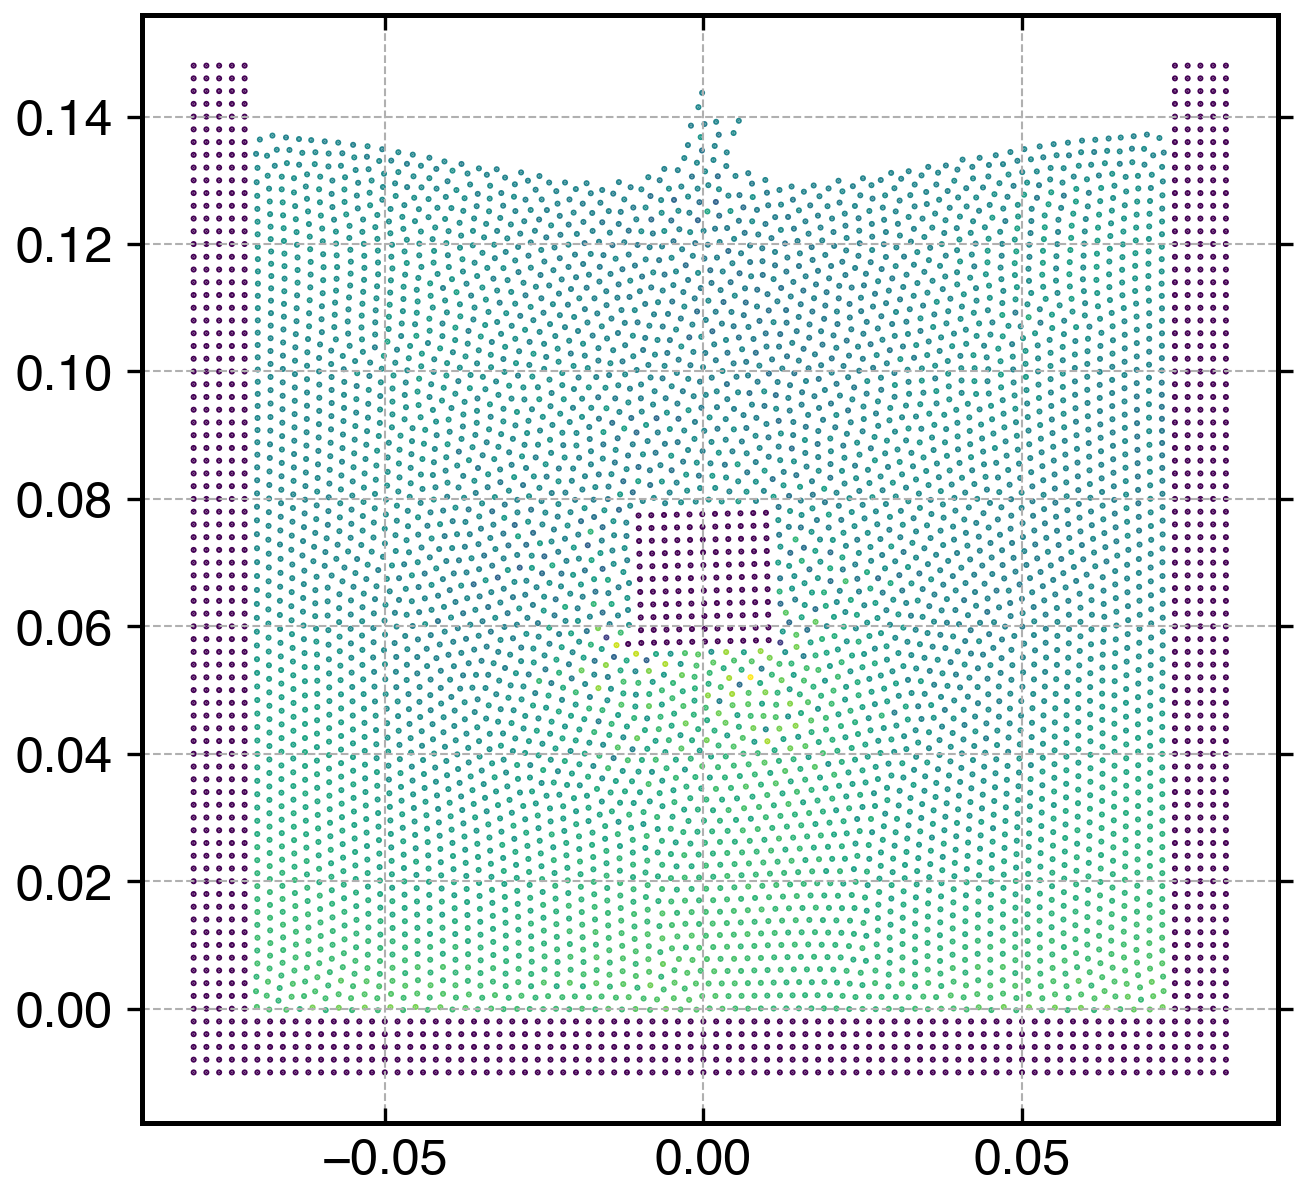
\includegraphics[width=1.0\textwidth]{figures/rfc/figures/qiu_2017_falling_solid_in_water_2d/dx_0_002/time1}
    \subcaption{t = $0.2$ sec}
  \end{subfigure}

  \begin{subfigure}{0.48\textwidth}
    \centering
    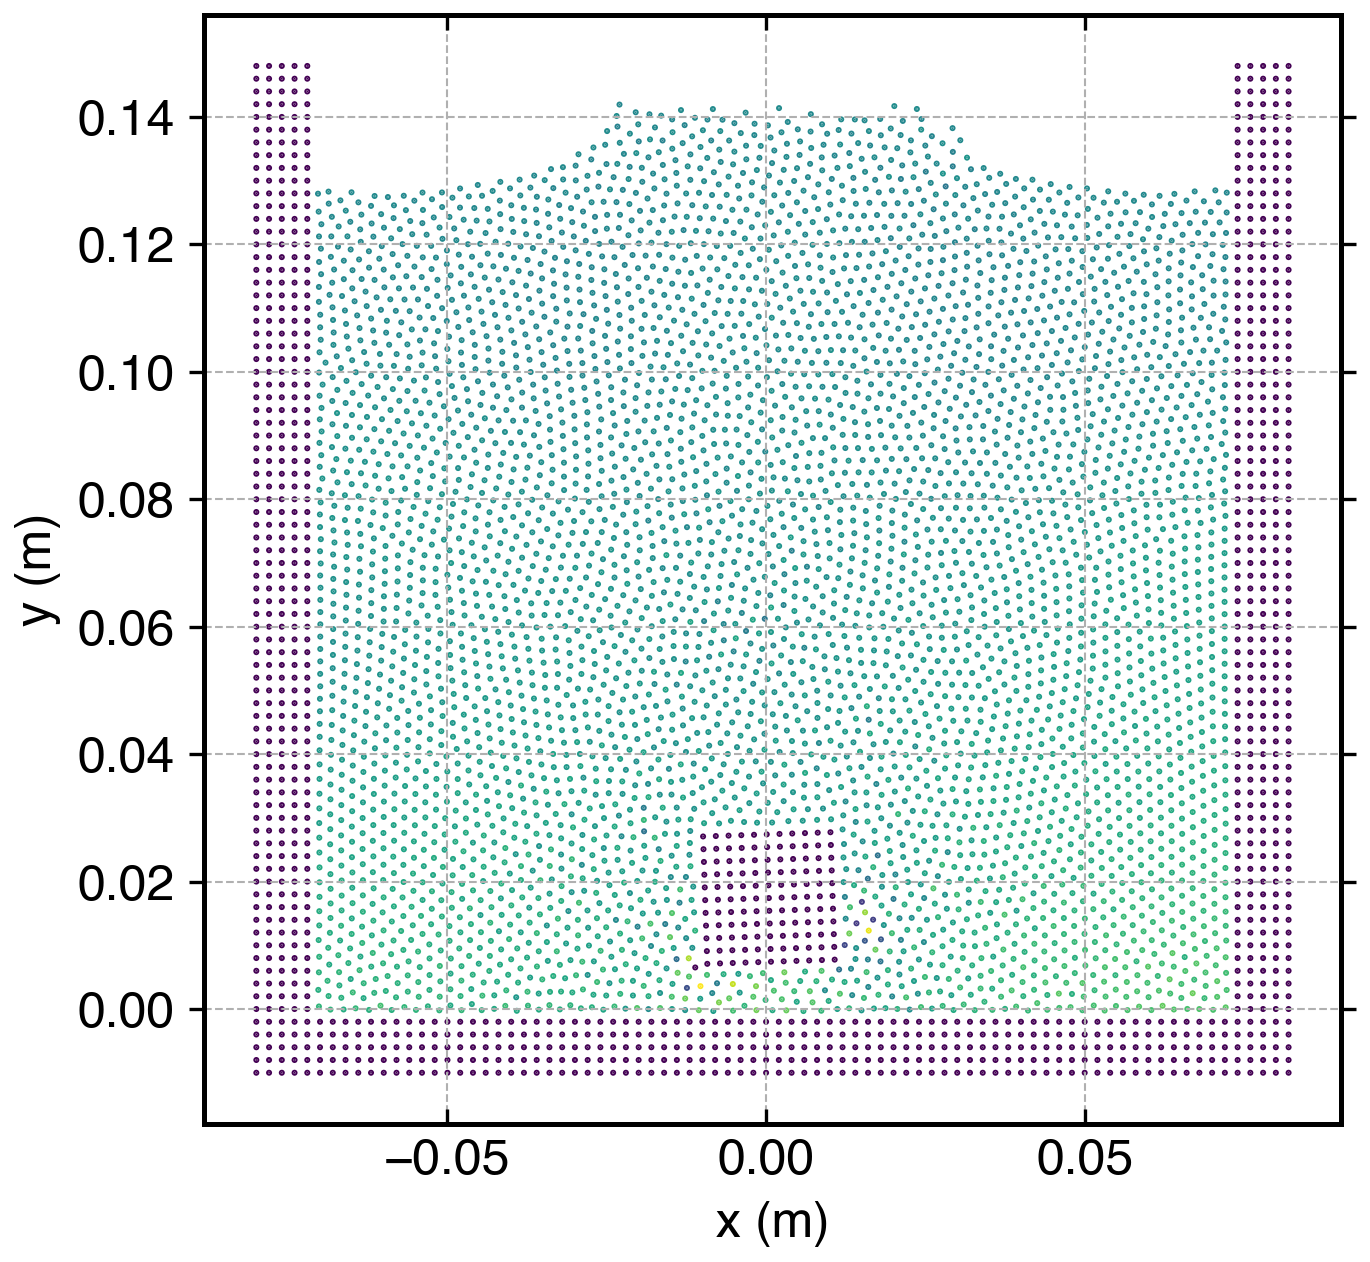
\includegraphics[width=1.0\textwidth]{figures/rfc/figures/qiu_2017_falling_solid_in_water_2d/dx_0_002/time2}
    \subcaption{t = $0.3$ sec}
  \end{subfigure}
  %
  \begin{subfigure}{0.48\textwidth}
    \centering
    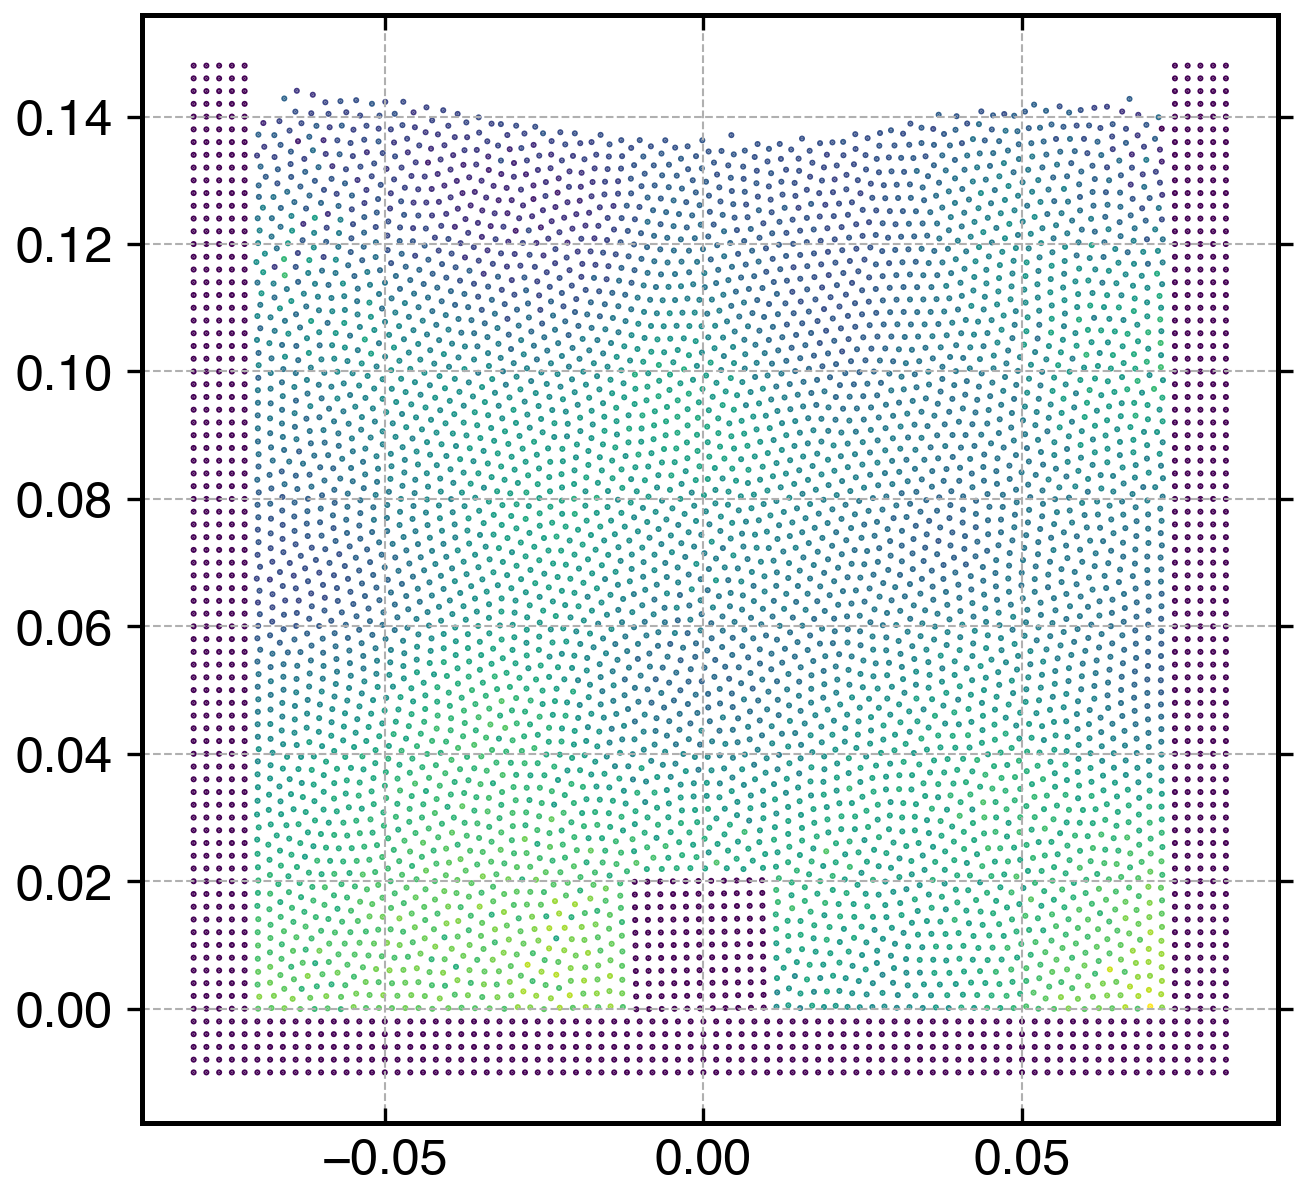
\includegraphics[width=1.0\textwidth]{figures/rfc/figures/qiu_2017_falling_solid_in_water_2d/dx_0_002/time4}
    \subcaption{t = $0.5$ sec}
  \end{subfigure}
\caption{}
\label{fig:snapshots-falling-solid-in-water}
\end{figure}
\Cref{fig:disp-falling-solid-in-water} presents the time history of the
displacement of the rigid cube with time in comparison with the experimental
result by (citep experimental paper). From the presented figure, the CTVF-DEM
model has reproduced the displacement of the rigid cube with acceptable levels
of stability as well as accuracy.
\begin{figure}[!htpb]
  \centering
  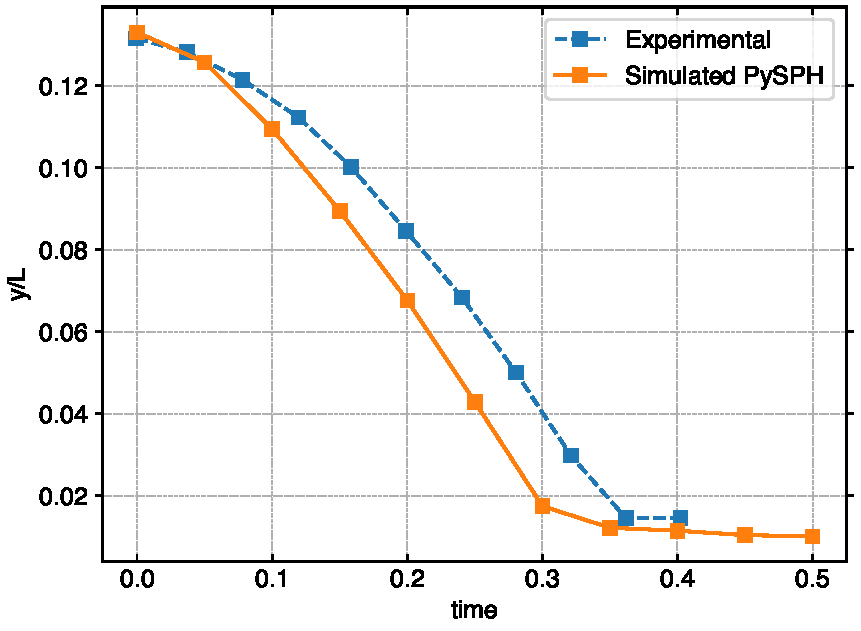
\includegraphics[width=0.4\textwidth]{figures/rfc/figures/qiu_2017_falling_solid_in_water_2d/y_cm_vs_time}
  \caption{Snapshots of the rigid cube entering a hydrostatic tank at four
    different time instants simulated with the current solver.}
\label{fig:disp-falling-solid-in-water}
\end{figure}


% \FloatBarrier%
% \subsection{Floating solid in water, 500 density cube}
% \label{sec:floating-solid-in-water}

% To be done



% \FloatBarrier%
% \subsection{A rigid box rotating and sinking in viscous liquid}
% Rotating box in fluid \citep{sun2015numerical}.


% \FloatBarrier%
% \subsection{Water entry of 2-D cylinder}
% Water entry of 2-D cylinder \citep{sun2015numerical}.


% \FloatBarrier%
% \subsection{2d wedge entry in water}
% \label{sec:wedge-entry-in-water}

% To be done

\FloatBarrier%
\subsection{Water-entry of a single sphere}
\label{sec:water-entry-sphere}
% https://www.sciencedirect.com/science/article/pii/S0997754621001412#fig2

In this section we reproduce the water entry of a single sphere experiment
done by \citep{aristoff_water_2010}. A sphere of diameter $24.4$ mm is allowed
to settle under gravity in a water tank of dimensions, $0.2$ m $\times$ $0.2$
m $\times$ $0.14$ m, with a water depth of $0.11$ m
(\cref{fig:water-entry-sphere-schematic}). The initial velocity of the sphere
is $2.17$ m/s. A convergence study of the current rigid fluid coupling
algorithm is carried out by simulating a total of 3 resolution studies ($0.01$
m, $0.005$ m, $0.002$ m) is carried out.
\begin{figure}[!htpb]
  \centering
  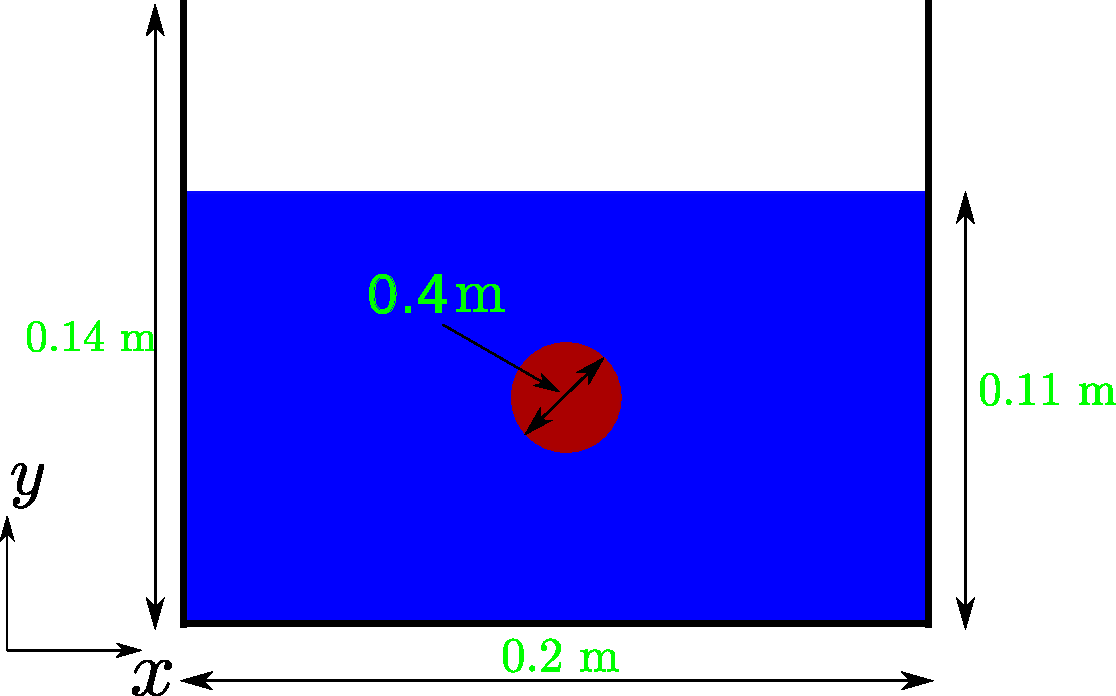
\includegraphics[width=0.4\textwidth]{images/rfc/images/water_entry_of_sphere/schematic}
  \caption{}
\label{fig:water-entry-sphere-schematic}
\end{figure}

\begin{figure}[!htpb]
  \centering
  \begin{subfigure}{0.48\textwidth}
    \centering
    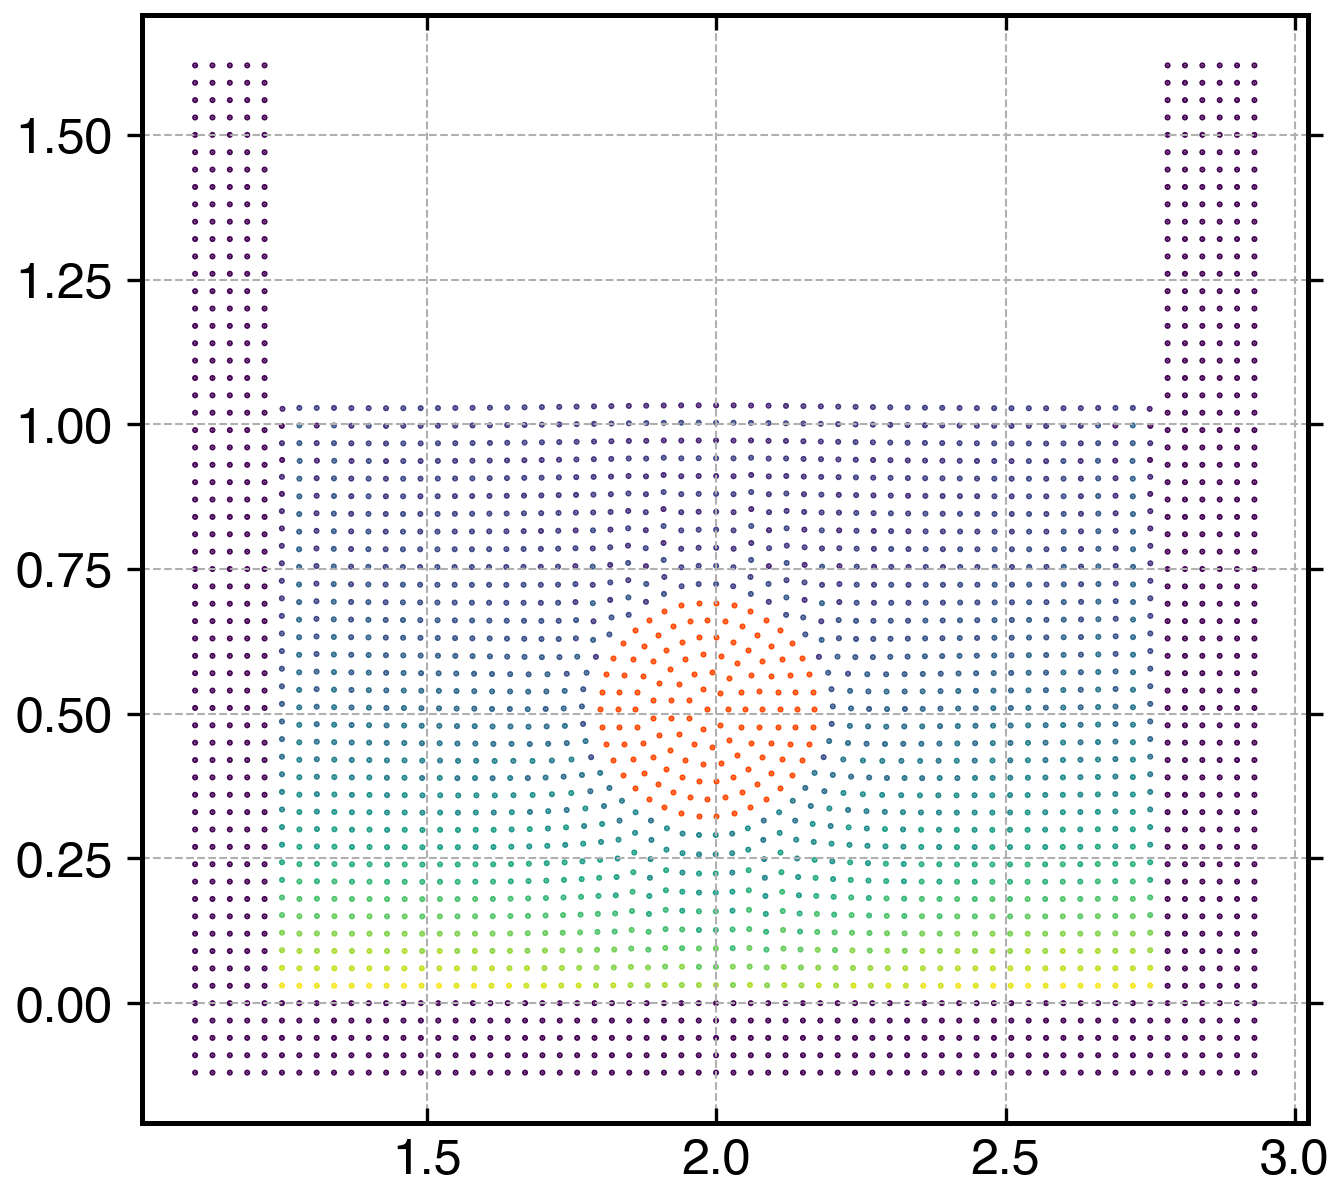
\includegraphics[width=1.0\textwidth]{figures/rfc/figures/dinesh_2022_body_in_hs_tank_2d/time1}
    \subcaption{t = $0$ sec}
  \end{subfigure}
  %
  \begin{subfigure}{0.48\textwidth}
    \centering
    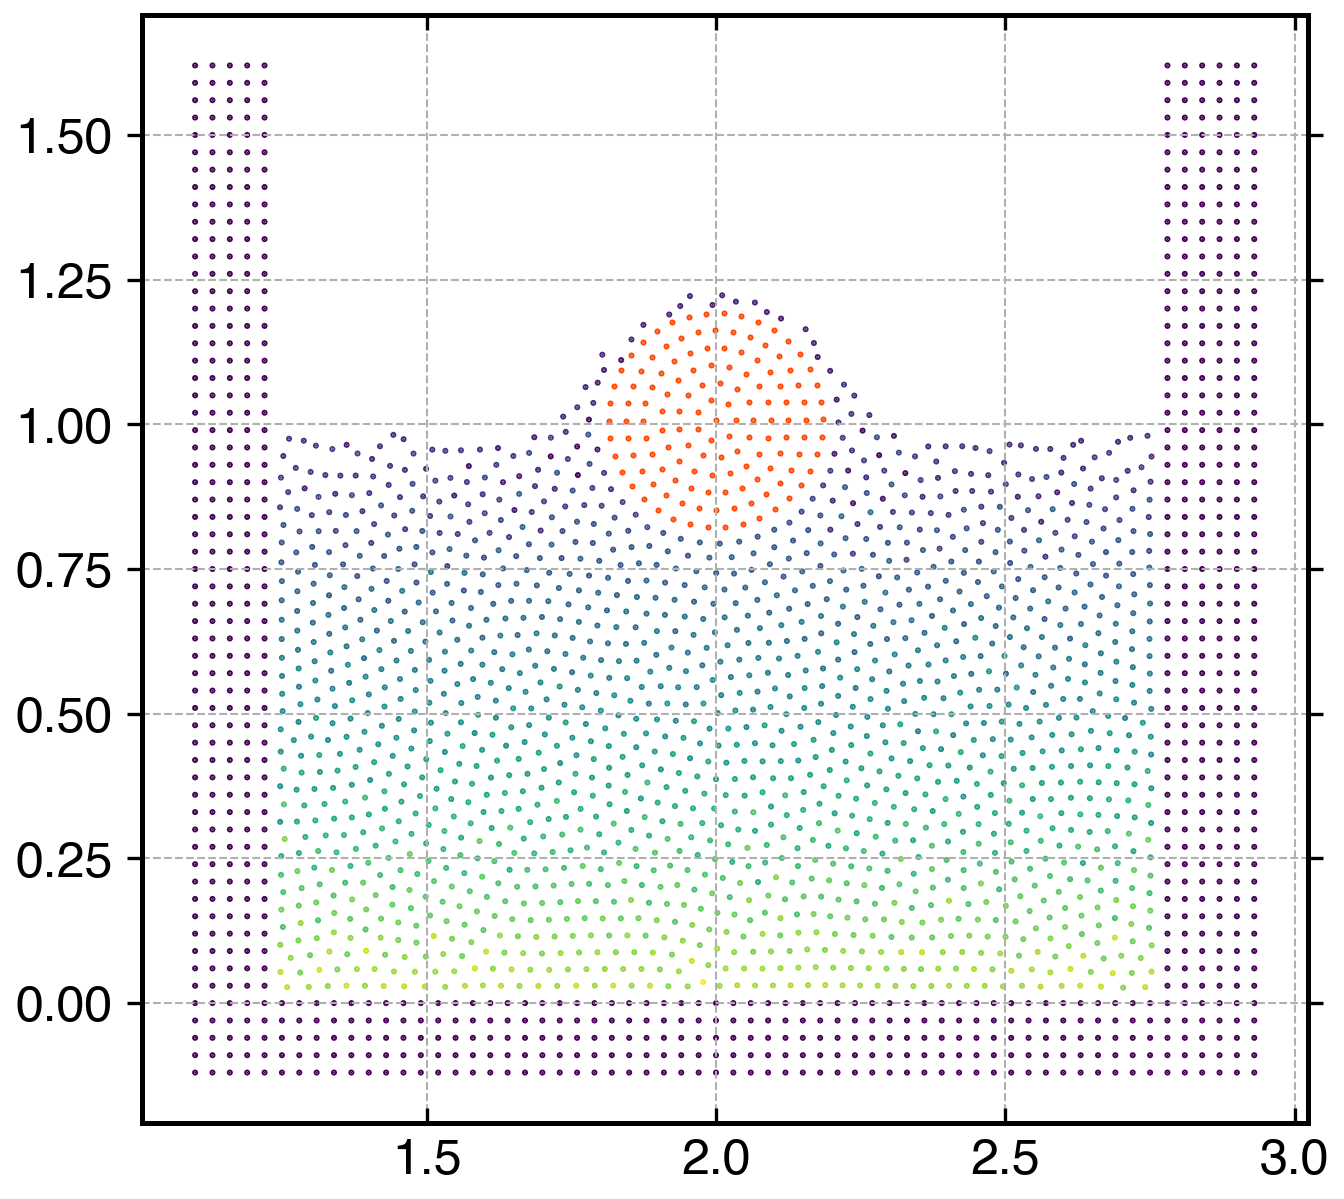
\includegraphics[width=1.0\textwidth]{figures/rfc/figures/dinesh_2022_body_in_hs_tank_2d/time4}
    \subcaption{t = $0$ sec}
  \end{subfigure}

  \begin{subfigure}{0.48\textwidth}
    \centering
    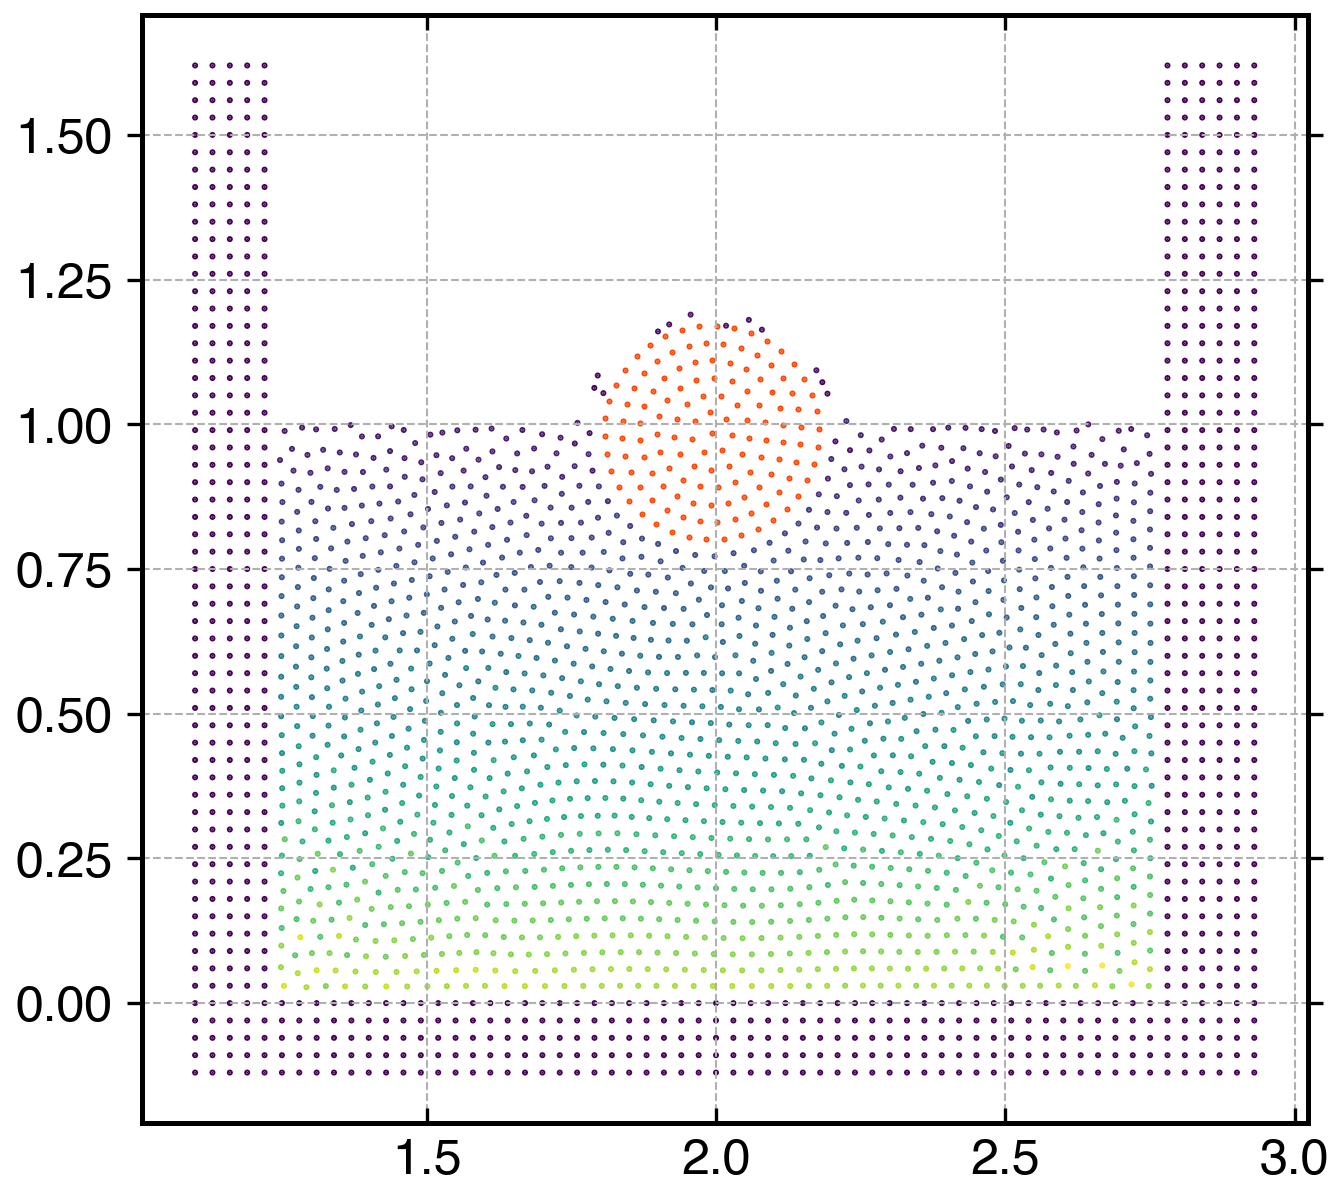
\includegraphics[width=1.0\textwidth]{figures/rfc/figures/dinesh_2022_body_in_hs_tank_2d/time6}
    \subcaption{t = $0$ sec}
  \end{subfigure}
  %
  \begin{subfigure}{0.48\textwidth}
    \centering
    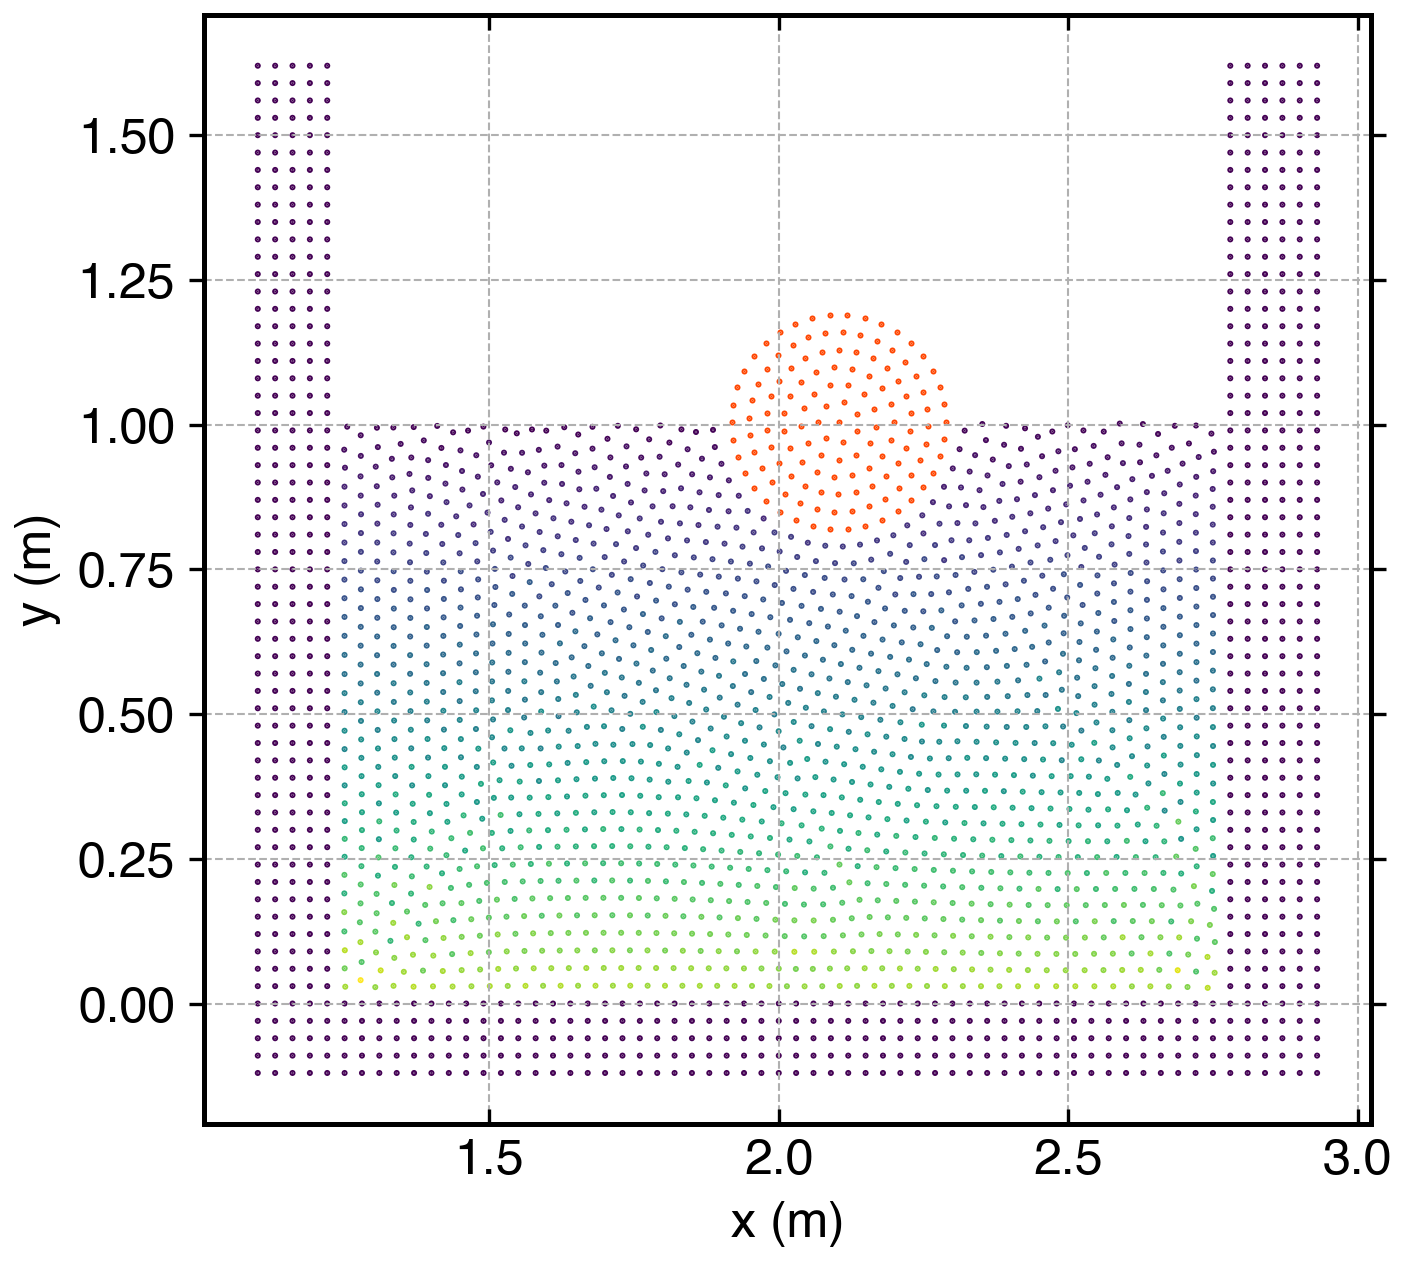
\includegraphics[width=1.0\textwidth]{figures/rfc/figures/dinesh_2022_body_in_hs_tank_2d/time11}
    \subcaption{t = $0$ sec}
  \end{subfigure}
  \caption{Snapshots of a 2D-cylinder of density $500$ kg\textsuperscript{-3}
    rising in a hydrostatic tank at four different time instants simulated
    with the current solver.}
\label{fig:snapshots-rising-solid-in-water}
\end{figure}

\begin{figure}[!htpb]
  \centering
  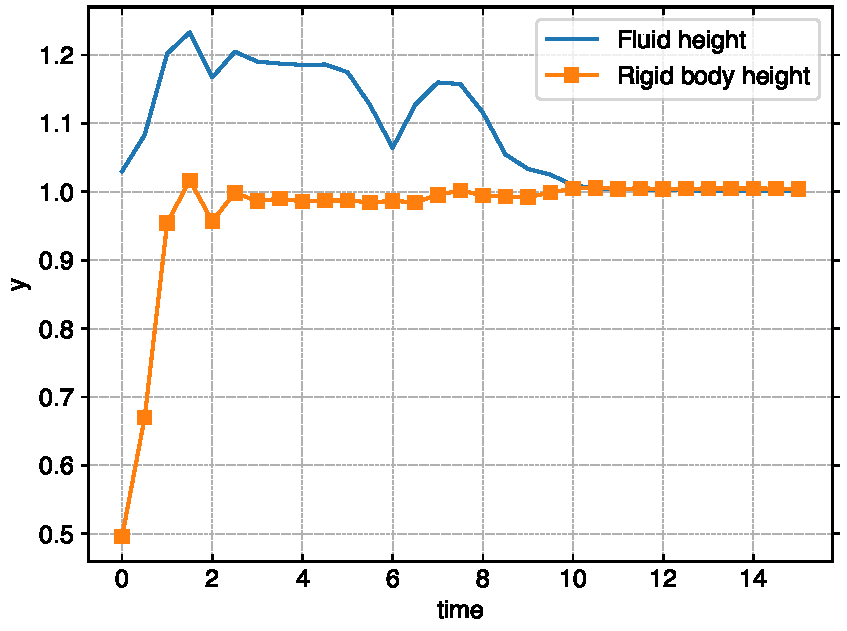
\includegraphics[width=0.4\textwidth]{figures/rfc/figures/dinesh_2022_body_in_hs_tank_2d/ycom}
  \caption{}
\label{fig:disp-falling-solid-in-water}
\end{figure}


% \FloatBarrier%
% \subsection{Settling of two identical cylinders in series}
% \label{sec:water-entry-sphere}
% % https://www.sciencedirect.com/science/article/pii/S0997754621001412#fig2

% In this section we reproduce the water entry of a single sphere experiment
% done by \citep{aristoff_water_2010}. A sphere of diameter $24.4$ mm is allowed
% to settle under gravity in a water tank of dimensions, $0.2$ m $\times$ $0.2$
% m $\times$ $0.14$ m, with a water depth of $0.11$ m
% (\cref{fig:cylinders-in-series-schematic}). The initial velocity of the sphere
% is $2.17$ m/s. A convergence study of the current rigid fluid coupling
% algorithm is carried out by simulating a total of 3 resolution studies ($0.01$
% m, $0.005$ m, $0.002$ m) is carried out.
% \begin{figure}[!htpb]
%   \centering
%   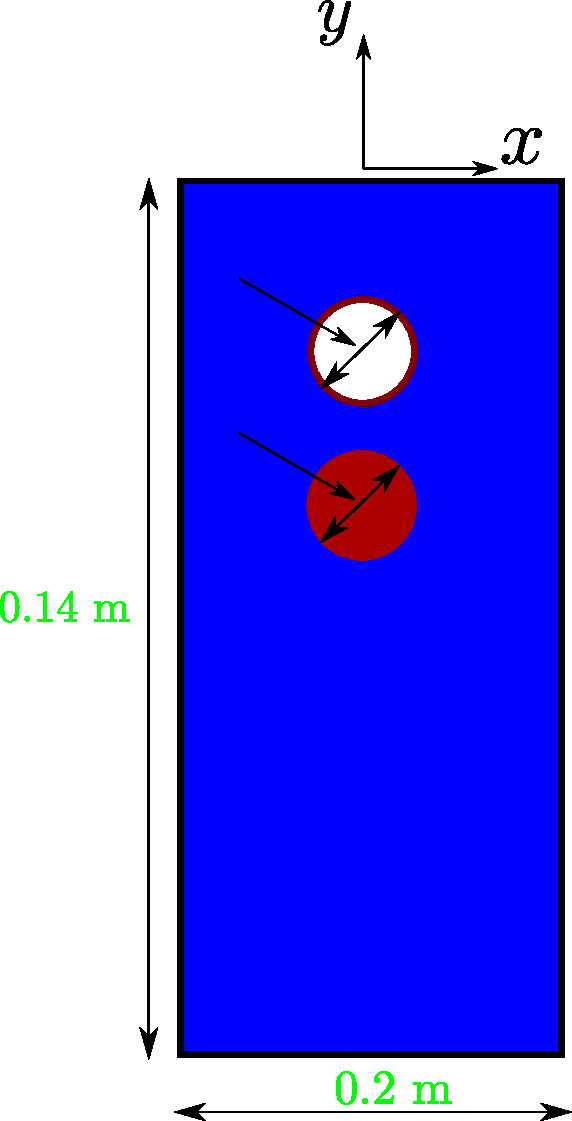
\includegraphics[width=0.4\textwidth]{images/rfc/images/two_cylinders_one_top_of_another/schematic}
%   \caption{Schematic}
% \label{fig:cylinders-in-series-schematic}
% \end{figure}


% \FloatBarrier%
% \subsection{Two identical spheres settlement side by side}
% \label{sec:water-entry-sphere}
% % https://www.sciencedirect.com/science/article/pii/S0997754621001412#fig2

% In this test we study the behaviour of two spheres setting inside a fluid
% tank. This test comprises of complex rigid-fluid coupling phenomena as well as
% the rigid interaction between the spheres. The dimensions of the sphere and
% % the fluid including the tank are shown in \cref{}.

% The initial velocity of the sphere is $2.17$ m/s. A convergence
% study of the current rigid fluid coupling algorithm is carried out by
% simulating a total of 3 resolution studies ($0.01$ m, $0.005$ m, $0.002$ m) is
% carried out.


% \FloatBarrier%
% \subsection{3D dam breaking flow hitting cubes}

% \citep{amaro2019improvement}

% In the current case we simulate a 3d dam breaking flow hitting different
% configuration of rigid cubes. This is experimentally studied by SPH DCDEM,
% where the author used Direct Linear Transform (DLT) to track the cubes as they
% move after the impact. A total three rigid body configurations are studied, a
% single cube, three cubes and a pyramid configuration, respectively. It is
% numerically studied by SPH-DCDEM, MPS-DEM, and (citep some other papers). The
% side length of each cube is $3.5$ mm and the material properties are listed in
% \cref{tab:material-properties-3d-dam-breaking-flow-hitting-cubes} and the
% numerical parameters are given in
% \cref{tab:material-properties-3d-dam-breaking-flow-hitting-cubes}. In all the
% three cases the fluid is initially allowed to flow by opening a gate which
% lifts at a velocity of 3.5 m\,s\textsuperscript{-1}

% \begin{table}[!ht]
%   \centering
%   \begin{tabular}[!ht]{ll}
%     \toprule
%     Quantity & Values\\
%     \midrule
%     $L$, length of the domain & 1 m \\
%     $\rho_0$, reference density & 1 kg/m\textsuperscript{3} \\
%     Reynolds number & 200 \& 1000 \\
%     Resolution, $L/\Delta x_{\max} : L/\Delta x_{\min}$ & $[100:200]$ \& $[150:300]$\\
%     \bottomrule
%   \end{tabular}
%   \caption{Parameters used for the Taylor-Green vortex problem.}%
%   \label{tab:material-properties-3d-dam-breaking-flow-hitting-cubes}
% \end{table}

% \begin{table}[!ht]
%   \centering
%   \begin{tabular}[!ht]{ll}
%     \toprule
%     Quantity & Values\\
%     \midrule
%     $L$, length of the domain & 1 m \\
%     $\rho_0$, reference density & 1 kg/m\textsuperscript{3} \\
%     Reynolds number & 200 \& 1000 \\
%     Resolution, $L/\Delta x_{\max} : L/\Delta x_{\min}$ & $[100:200]$ \& $[150:300]$\\
%     \bottomrule
%   \end{tabular}
%   \caption{Parameters used for the Taylor-Green vortex problem.}%
%   \label{tab:numerical-properties-3d-dam-breaking-flow-hitting-cubes}
% \end{table}

% \Cref{fig:snapshots-single-cube-3d-dam-breaking-flow} shows the snapshots of
% the rigid cube moving downstream of the tank when interacting with the fluid
% flow against the experimental result (citep SPH DCDEM). From
% \Cref{fig:snapshots-single-cube-3d-dam-breaking-flow} we can see that the
% rigid cube matches well with the experimental result. Further, we compare the
% positions of the rigid cube with time in
% \Cref{fig:x-position-single-cube-3d-dam-breaking-flow}, against the
% experimental results, SPH-DCDEM, MPS-DEM results. It can be seen from figure
% \Cref{fig:x-position-single-cube-3d-dam-breaking-flow} that the current solver
% is able to provide good accuracy in producing the correct displacement of the
% cube and agrees well with the experimental as well as the other numerical
% techniques.
% \begin{figure}[!htpb]
%   \centering
%   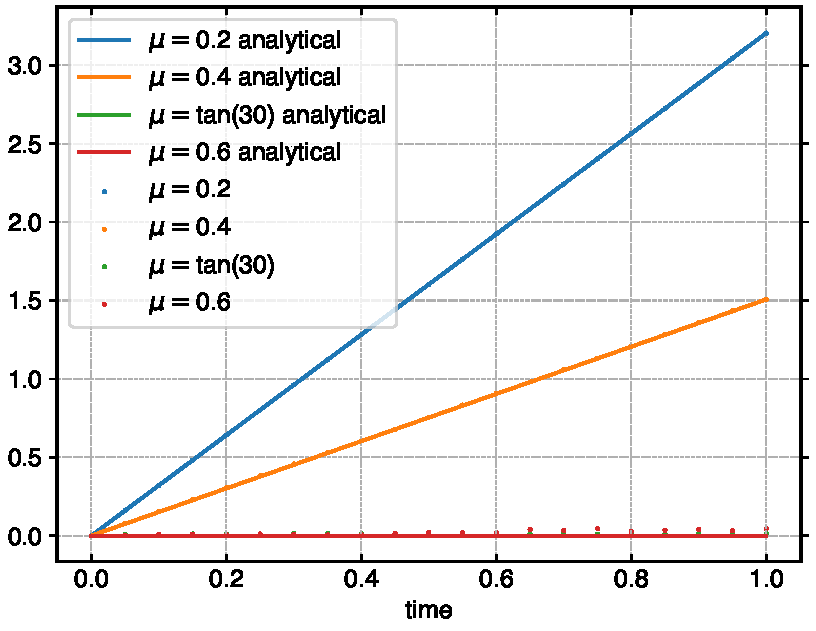
\includegraphics[width=0.4\textwidth]{figures/rfc/figures/mohseni_2021_free_sliding_on_a_slope_3d/velocity_vs_time}
%   \caption{Snapshots of a single cube under a 3d dam breaking flow}
% \label{fig:snapshots-single-cube-3d-dam-breaking-flow}
% \end{figure}
% \begin{figure}[!htpb]
%   \centering
%   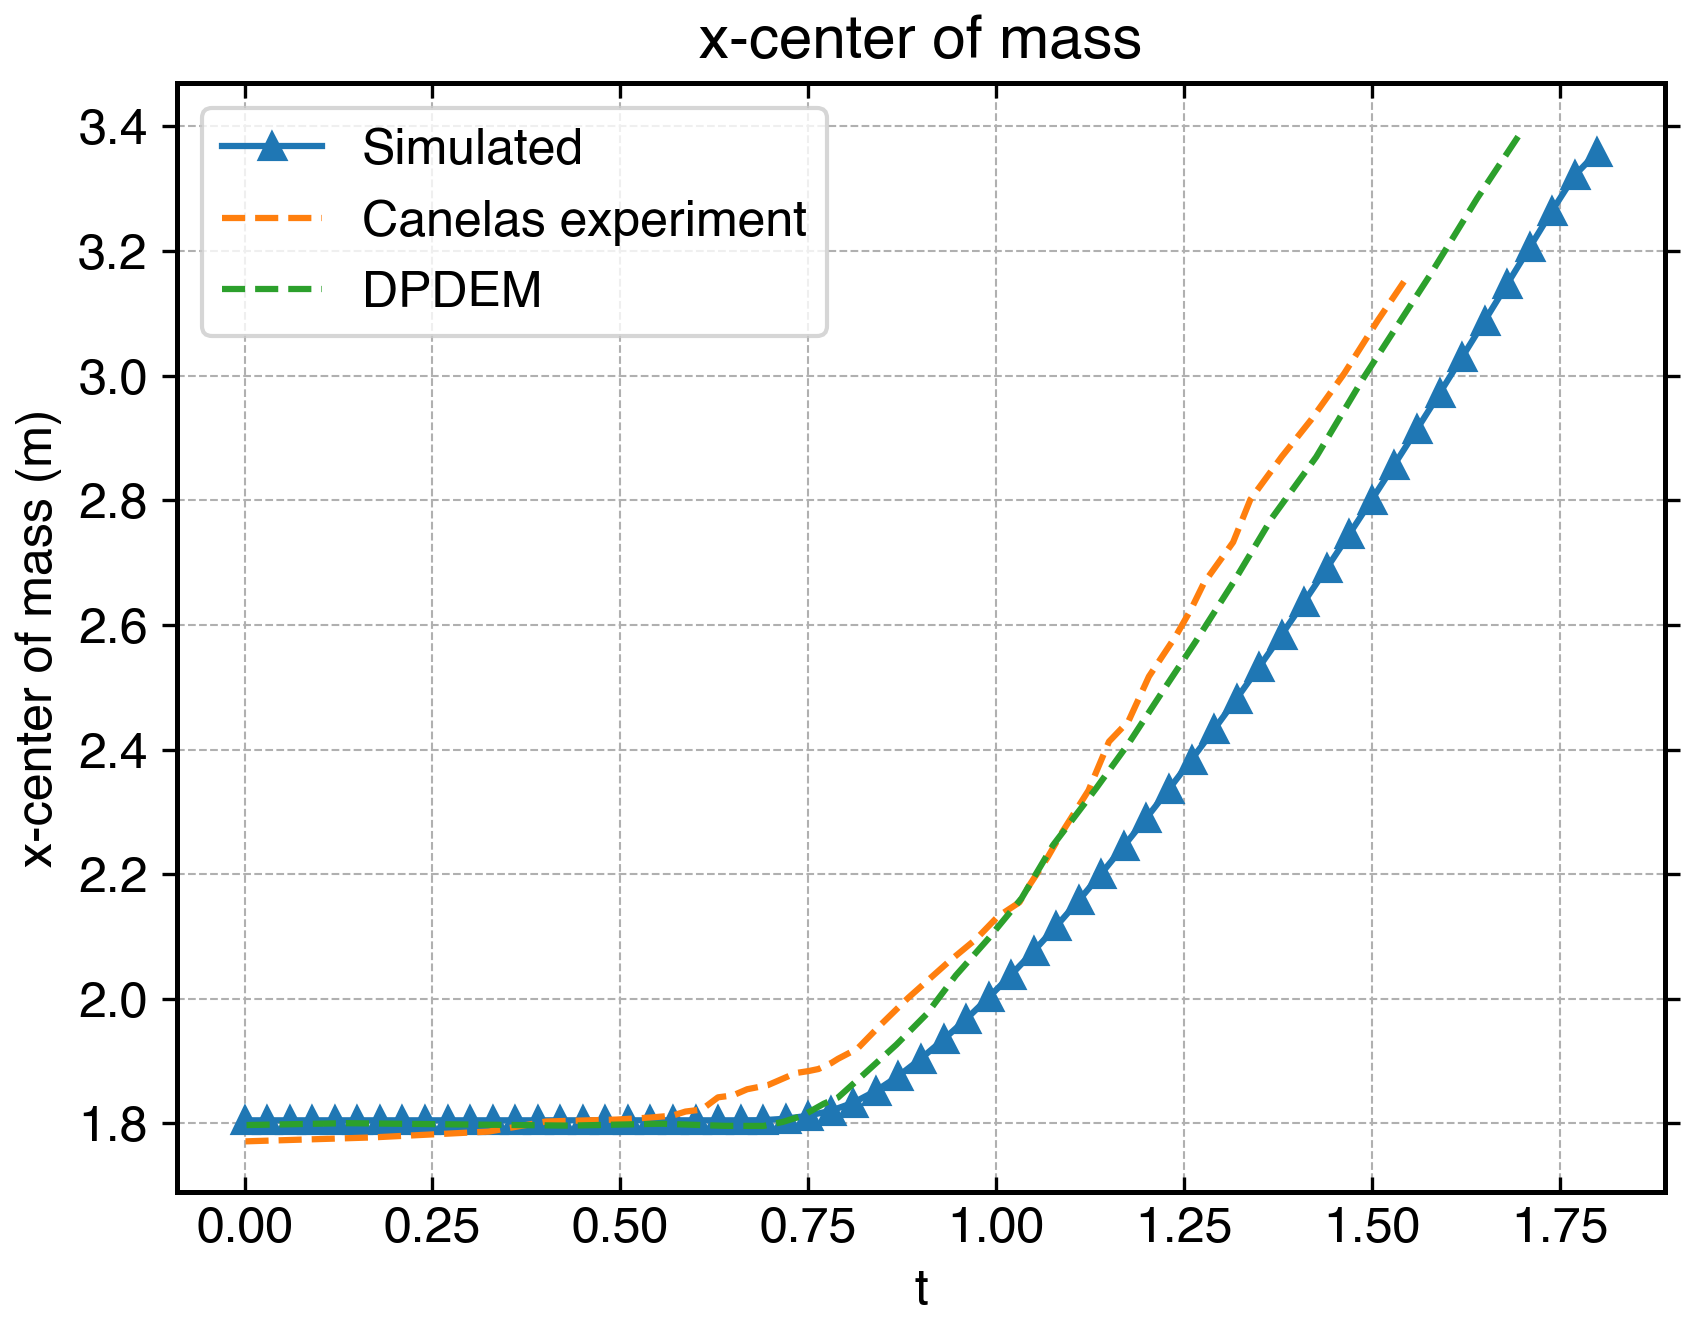
\includegraphics[width=0.4\textwidth]{figures/rfc/figures/amaro_2019_dam_breaking_flow_hitting_one_cube_3d/case_1/xcom_vs_time}
%   \caption{x position of the cube with time for single cube.}
% \label{fig:x-position-single-cube-3d-dam-breaking-flow}
% \end{figure}

% The initial configuration of the dam breaking flow over three cubes is shown
% in figure \Cref{fig:snapshots-three-cubes-3d-dam-breaking-flow}.
% \Cref{fig:snapshots-three-cubes-3d-dam-breaking-flow} shows the snapshots of
% the rigid cubes at different time instants from the start of fluid hit with
% the color of the fluid particles representing pressure. From the
% \Cref{fig:snapshots-three-cubes-3d-dam-breaking-flow} we can see that the
% simulated rigid bodies match well with the experimental observations. We also
% compare the x component of the effective center of mass of the three cubes
% with time in \Cref{fig:x-position-three-cubes-3d-dam-breaking-flow}, against
% the experimental results, SPH-DCDEM, MPS-DEM results. From figure
% \Cref{fig:x-position-three-cubes-3d-dam-breaking-flow}, we can see that the
% current solve is agrees well with the experimental as well as with the other
% numerical method results.
% \begin{itemize}
% \item Mention at what time does the fluid hits the rigid cubes.
% \end{itemize}
% \begin{figure}[!htpb]
%   \centering
%   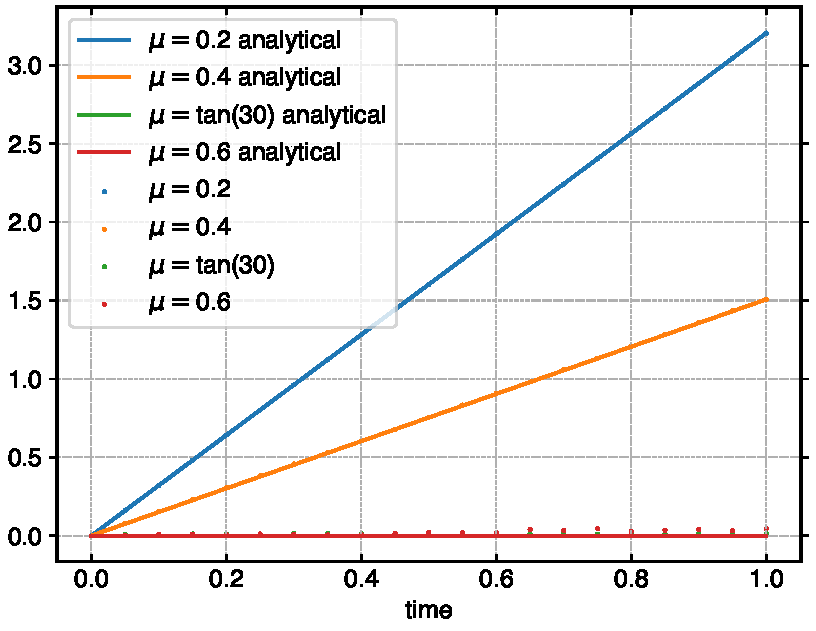
\includegraphics[width=0.4\textwidth]{figures/rfc/figures/mohseni_2021_free_sliding_on_a_slope_3d/velocity_vs_time}
%   \caption{Snapshots of a three cubes under a 3d dam breaking flow}
% \label{fig:snapshots-three-cubes-3d-dam-breaking-flow}
% \end{figure}
% \begin{figure}[!htpb]
%   \centering
%   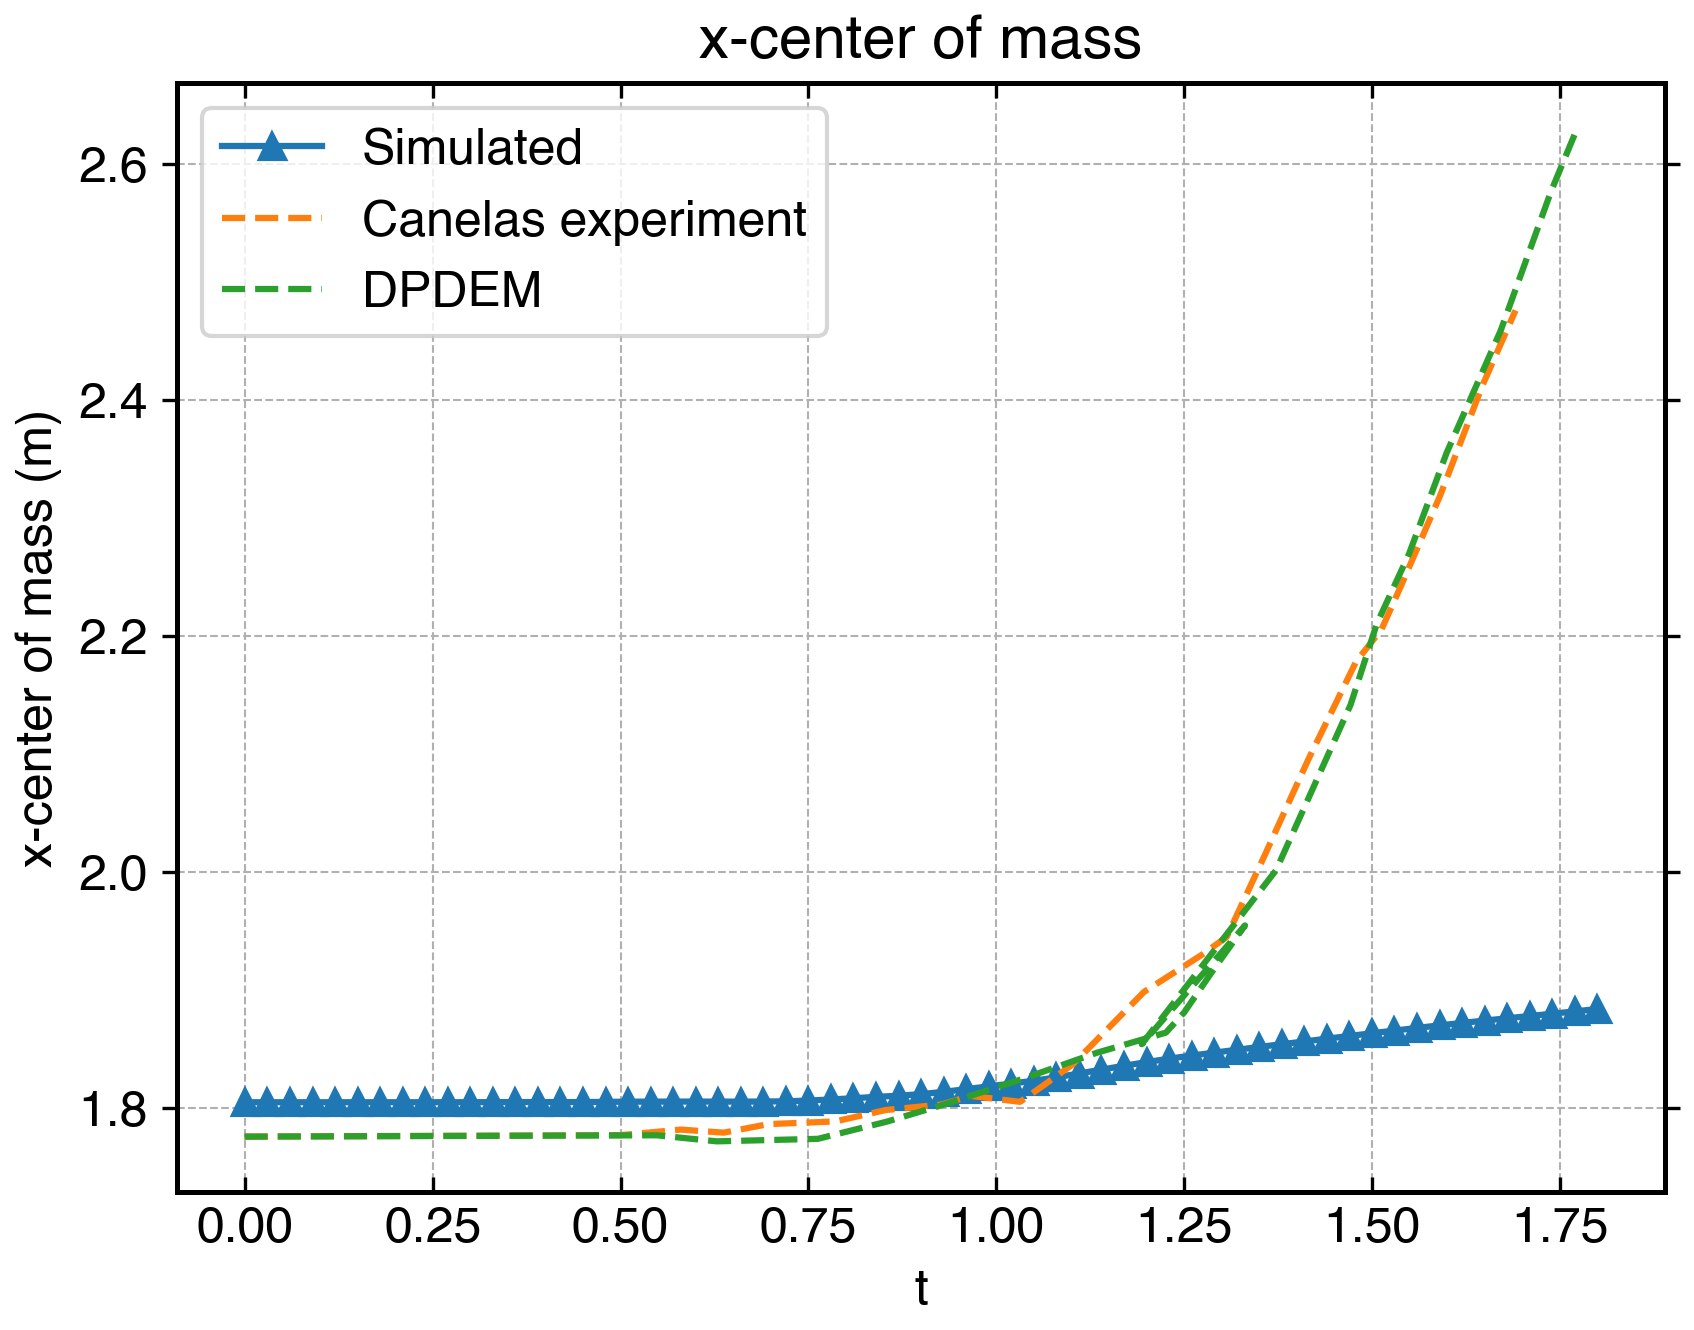
\includegraphics[width=0.4\textwidth]{figures/rfc/figures/amaro_2019_dam_breaking_flow_hitting_three_stacked_cubes_3d/case_1/xcom_vs_time}
%   \caption{x position of the cubes with time for three cube.}
% \label{fig:x-position-three-cubes-3d-dam-breaking-flow}
% \end{figure}
% \begin{figure}[!htpb]
%   \centering
%   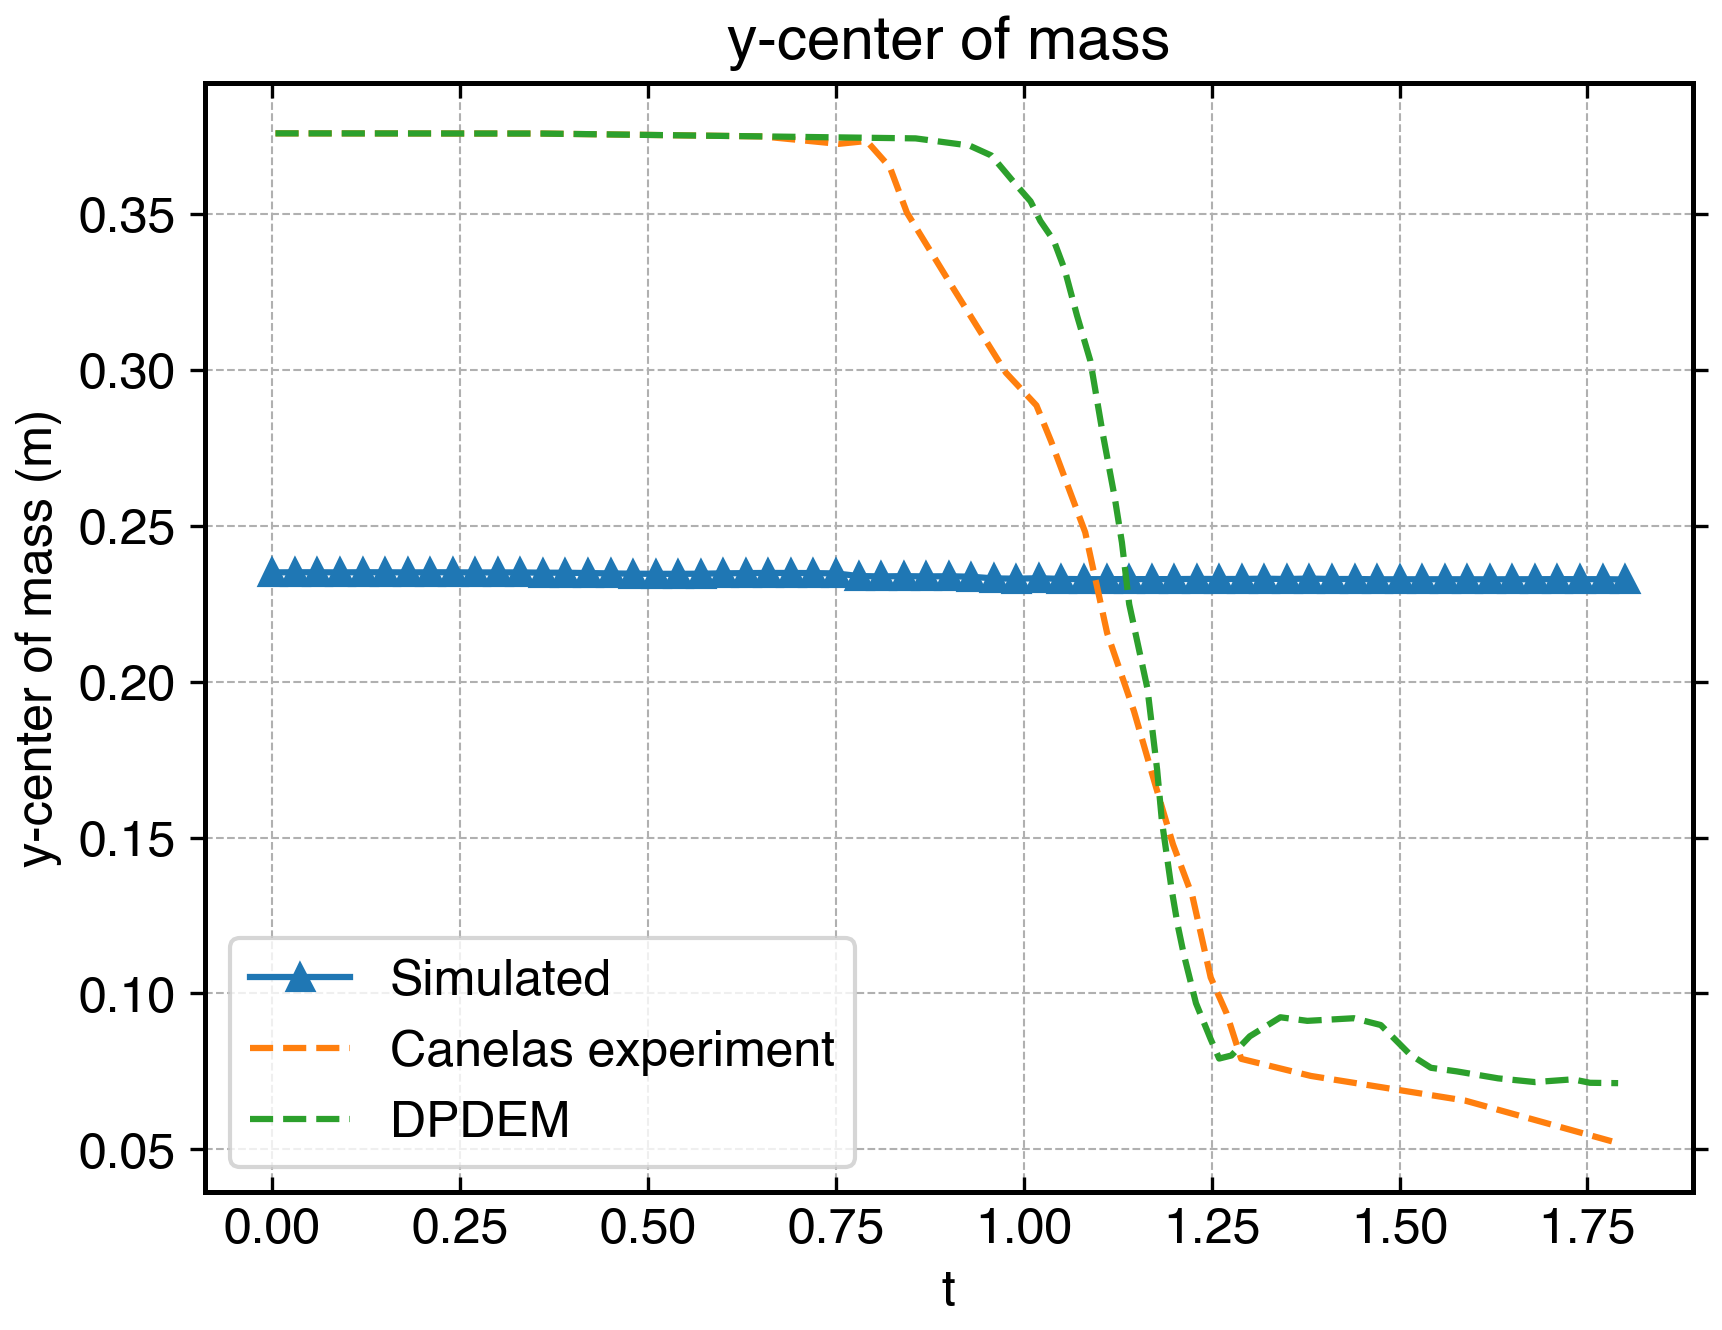
\includegraphics[width=0.4\textwidth]{figures/rfc/figures/amaro_2019_dam_breaking_flow_hitting_three_stacked_cubes_3d/case_1/ycom_vs_time}
%   \caption{y position of the cubes with time for three cube.}
% \label{fig:y-position-three-cubes-3d-dam-breaking-flow}
% \end{figure}


% The placement of the cubes in the pyramid configuration including dimensions,
% distance from the left wall and other dimension related information can be
% seen in figure \Cref{fig:snapshots-three-cubes-3d-dam-breaking-flow}.
% \Cref{fig:snapshots-three-cubes-3d-dam-breaking-flow} shows the snapshots of
% the rigid cubes at different time instants and the color coding of the fluid
% particles represents pressure. From
% \Cref{fig:snapshots-three-cubes-3d-dam-breaking-flow}, it can be seen that the
% rigid body positions are in match with the experimental observations. Which is
% further validated by doing a quantitative comparison of the x component of
% effective center of mass of the six cubes in time against the experimental
% results, SPH-DCDEM, MPS-DEM results in
% \Cref{fig:x-position-six-cubes-3d-dam-breaking-flow}. From these figures, we
% can see that the current solver is in good agreement with the other numerical
% and experimental results.
% \begin{figure}[!htpb]
%   \centering
%   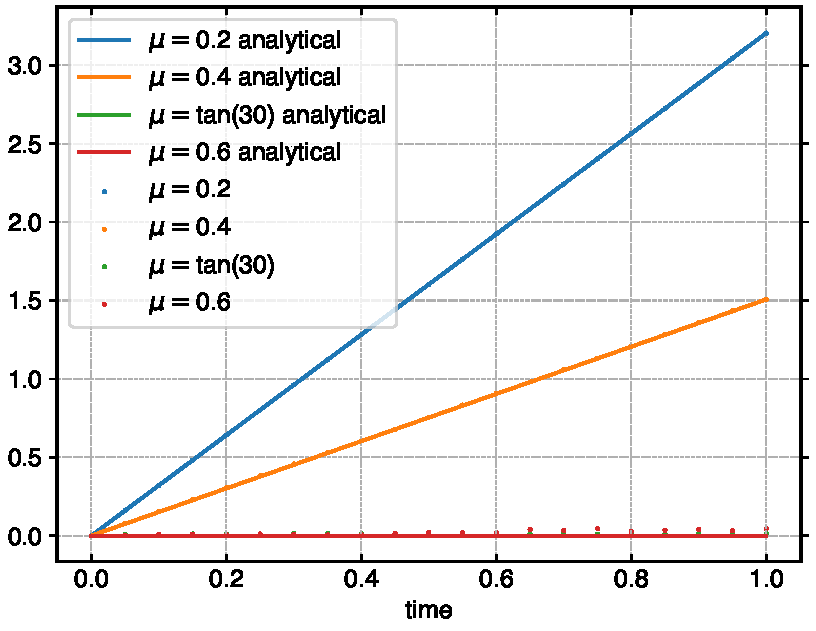
\includegraphics[width=0.4\textwidth]{figures/rfc/figures/mohseni_2021_free_sliding_on_a_slope_3d/velocity_vs_time}
%   \caption{Snapshots of six cubes under a 3d dam breaking flow}
% \label{fig:snapshots-six-cubes-3d-dam-breaking-flow}
% \end{figure}
% \begin{figure}[!htpb]
%   \centering
%   \includegraphics[width=0.4\textwidth]{figures/rfc/figures/amaro_2019_dam_breaking_flow_hitting_six_stacked_cubes_3d/case_1/xcom_vs_time}
%   \caption{x position of the cubes with time for six cubes.}
% \label{fig:x-position-six-cubes-3d-dam-breaking-flow}
% \end{figure}
% \begin{figure}[!htpb]
%   \centering
%   \includegraphics[width=0.4\textwidth]{figures/rfc/figures/amaro_2019_dam_breaking_flow_hitting_six_stacked_cubes_3d/case_1/ycom_vs_time}
%   \caption{y position of the cubes with time for six cubes.}
% \label{fig:y-position-six-cubes-3d-dam-breaking-flow}
% \end{figure}


% \subsection{Dam break with body transport}
% \label{sec:dam-break-with-body-transport}

% \cite{wang2019numerical}

% \subsection{Dam break with multiple bodies transport}
% \label{sec:dam-break-with-multiple-bodies-transport}
% \cite{wang2019numerical}


% \subsection{Cylinders in water collapsed under gravity}
% \label{sec:cylinders-collapse-in-water}
% \cite{chen2019coupled}


\FloatBarrier%
\section{Summary}
\label{sec:Summary}
A coupled solver, CTVF-DEM is developed to simulate a two-way rigid-fluid
coupling phenomenon. The fluid phase is handled by the CTVF scheme, while DEM is
used to handle the interaction between the arbitrarily shaped rigid bodies. A
modified contact force formulation is utilized in DEM to handle the contact
between the arbitrarily shaped bodies.

It has been demonstrated that the current model is able to predict behaviour of
rigid bodies under the influence of fluid flow with different test cases. A
square cube sliding down an inclined plane is simulated to test the interaction
model between the rigid bodies. Different test cases are used to test the rigid
-fluid coupling phenomenon. Water entry and rising of solid bodies is studied as
part of the rigid-fluid coupling analysis.
% Finally, the full scale model is applied to study
% the transport of rigid body under dam-breaking event and compared against the
% experimental counterpart.
Further, we have made our implementation open-source and fully reproducible.

With the completion of modeling fluid, elastic, fluid-structure and the contact
between the solids, in the current chapter we have modeled dynamics of rigid
bodies in fluid flows and rigid-rigid interaction. In the next chapter we will
model the interaction between the rigid and a ductile target. The ductile target
is modelled assuming elastic-plastic, where the solver in \cref{chap:ctvf} is
extended to handle the plastic behaviour through Johnson-Cook constitutive
model.
